% Options for packages loaded elsewhere
\PassOptionsToPackage{unicode}{hyperref}
\PassOptionsToPackage{hyphens}{url}
\PassOptionsToPackage{dvipsnames,svgnames*,x11names*}{xcolor}
%
\documentclass[
  10pt,
  dvipsnames,enabledeprecatedfontcommands]{scrartcl}
\usepackage{amsmath,amssymb}
\usepackage{lmodern}
\usepackage{ifxetex,ifluatex}
\ifnum 0\ifxetex 1\fi\ifluatex 1\fi=0 % if pdftex
  \usepackage[T1]{fontenc}
  \usepackage[utf8]{inputenc}
  \usepackage{textcomp} % provide euro and other symbols
\else % if luatex or xetex
  \usepackage{unicode-math}
  \defaultfontfeatures{Scale=MatchLowercase}
  \defaultfontfeatures[\rmfamily]{Ligatures=TeX,Scale=1}
\fi
% Use upquote if available, for straight quotes in verbatim environments
\IfFileExists{upquote.sty}{\usepackage{upquote}}{}
\IfFileExists{microtype.sty}{% use microtype if available
  \usepackage[]{microtype}
  \UseMicrotypeSet[protrusion]{basicmath} % disable protrusion for tt fonts
}{}
\usepackage{xcolor}
\IfFileExists{xurl.sty}{\usepackage{xurl}}{} % add URL line breaks if available
\IfFileExists{bookmark.sty}{\usepackage{bookmark}}{\usepackage{hyperref}}
\hypersetup{
  pdftitle={Likelihood ratio and evidence strength},
  pdfauthor={Marcello Di Bello and Rafal Urbaniak},
  colorlinks=true,
  linkcolor=Maroon,
  filecolor=Maroon,
  citecolor=Blue,
  urlcolor=blue,
  pdfcreator={LaTeX via pandoc}}
\urlstyle{same} % disable monospaced font for URLs
\usepackage{graphicx}
\makeatletter
\def\maxwidth{\ifdim\Gin@nat@width>\linewidth\linewidth\else\Gin@nat@width\fi}
\def\maxheight{\ifdim\Gin@nat@height>\textheight\textheight\else\Gin@nat@height\fi}
\makeatother
% Scale images if necessary, so that they will not overflow the page
% margins by default, and it is still possible to overwrite the defaults
% using explicit options in \includegraphics[width, height, ...]{}
\setkeys{Gin}{width=\maxwidth,height=\maxheight,keepaspectratio}
% Set default figure placement to htbp
\makeatletter
\def\fps@figure{htbp}
\makeatother
\setlength{\emergencystretch}{3em} % prevent overfull lines
\providecommand{\tightlist}{%
  \setlength{\itemsep}{0pt}\setlength{\parskip}{0pt}}
\setcounter{secnumdepth}{5}
%\documentclass{article}

% %packages
 \usepackage{booktabs}
\usepackage{subcaption}
\usepackage{multirow}
\usepackage{colortbl}
\usepackage{graphicx}
\usepackage{longtable}
\usepackage{ragged2e}
\usepackage{etex}
%\usepackage{yfonts}
\usepackage{marvosym}
\usepackage[notextcomp]{kpfonts}
\usepackage{nicefrac}
\newcommand*{\QED}{\hfill \footnotesize {\sc Q.e.d.}}
\usepackage{floatrow}
%\usepackage[titletoc]{appendix}
%\renewcommand\thesubsection{\Alph{subsection}}

\usepackage[textsize=footnotesize]{todonotes}
\newcommand{\ali}[1]{\todo[color=gray!40]{#1}}
\newcommand{\mar}[1]{\todo[color=blue!40]{#1}}
\newcommand{\raf}[1]{\todo[color=olive!40]{#1}}
%\linespread{1.5}
\newcommand{\indep}{\!\perp \!\!\! \perp\!}


\setlength{\parindent}{10pt}
\setlength{\parskip}{1pt}


%language
\usepackage{times}
\usepackage{t1enc}
%\usepackage[utf8x]{inputenc}
%\usepackage[polish]{babel}
%\usepackage{polski}




%AMS
\usepackage{amsfonts}
\usepackage{amssymb}
\usepackage{amsthm}
\usepackage{amsmath}
\usepackage{mathtools}

\usepackage{geometry}
 \geometry{a4paper,left=35mm,top=20mm,}


%environments
\newtheorem{fact}{Fact}



%abbreviations
\newcommand{\ra}{\rangle}
\newcommand{\la}{\langle}
\newcommand{\n}{\neg}
\newcommand{\et}{\wedge}
\newcommand{\jt}{\rightarrow}
\newcommand{\ko}[1]{\forall  #1\,}
\newcommand{\ro}{\leftrightarrow}
\newcommand{\exi}[1]{\exists\, {_{#1}}}
\newcommand{\pr}[1]{\mathsf{P}(#1)}
\newcommand{\cost}{\mathsf{cost}}
\newcommand{\benefit}{\mathsf{benefit}}
\newcommand{\ut}{\mathsf{ut}}

\newcommand{\odds}{\mathsf{Odds}}
\newcommand{\ind}{\mathsf{Ind}}
\newcommand{\nf}[2]{\nicefrac{#1\,}{#2}}
\newcommand{\R}[1]{\texttt{#1}}
\newcommand{\prr}[1]{\mbox{$\mathtt{P}_{prior}(#1)$}}
\newcommand{\prp}[1]{\mbox{$\mathtt{P}_{posterior}(#1)$}}



\newtheorem{q}{\color{blue}Question}
\newtheorem{lemma}{Lemma}
\newtheorem{theorem}{Theorem}



%technical intermezzo
%---------------------

\newcommand{\intermezzoa}{
	\begin{minipage}[c]{13cm}
	\begin{center}\rule{10cm}{0.4pt}



	\tiny{\sc Optional Content Starts}
	
	\vspace{-1mm}
	
	\rule{10cm}{0.4pt}\end{center}
	\end{minipage}\nopagebreak 
	}


\newcommand{\intermezzob}{\nopagebreak 
	\begin{minipage}[c]{13cm}
	\begin{center}\rule{10cm}{0.4pt}

	\tiny{\sc Optional Content Ends}
	
	\vspace{-1mm}
	
	\rule{10cm}{0.4pt}\end{center}
	\end{minipage}
	}
%--------------------






















\newtheorem*{reply*}{Reply}
\usepackage{enumitem}
\newcommand{\question}[1]{\begin{enumerate}[resume,leftmargin=0cm,labelsep=0cm,align=left]
\item #1
\end{enumerate}}

\usepackage{float}

% \setbeamertemplate{blocks}[rounded][shadow=true]
% \setbeamertemplate{itemize items}[ball]
% \AtBeginPart{}
% \AtBeginSection{}
% \AtBeginSubsection{}
% \AtBeginSubsubsection{}
% \setlength{\emergencystretch}{0em}
% \setlength{\parskip}{0pt}






\usepackage[authoryear]{natbib}

%\bibliographystyle{apalike}



\usepackage{tikz}
\usetikzlibrary{positioning,shapes,arrows}

\usepackage{booktabs}
\usepackage{longtable}
\usepackage{array}
\usepackage{multirow}
\usepackage{wrapfig}
\usepackage{float}
\usepackage{colortbl}
\usepackage{pdflscape}
\usepackage{tabu}
\usepackage{threeparttable}
\usepackage{threeparttablex}
\usepackage[normalem]{ulem}
\usepackage{makecell}
\usepackage{xcolor}
\ifluatex
  \usepackage{selnolig}  % disable illegal ligatures
\fi
\newlength{\cslhangindent}
\setlength{\cslhangindent}{1.5em}
\newlength{\csllabelwidth}
\setlength{\csllabelwidth}{3em}
\newenvironment{CSLReferences}[2] % #1 hanging-ident, #2 entry spacing
 {% don't indent paragraphs
  \setlength{\parindent}{0pt}
  % turn on hanging indent if param 1 is 1
  \ifodd #1 \everypar{\setlength{\hangindent}{\cslhangindent}}\ignorespaces\fi
  % set entry spacing
  \ifnum #2 > 0
  \setlength{\parskip}{#2\baselineskip}
  \fi
 }%
 {}
\usepackage{calc}
\newcommand{\CSLBlock}[1]{#1\hfill\break}
\newcommand{\CSLLeftMargin}[1]{\parbox[t]{\csllabelwidth}{#1}}
\newcommand{\CSLRightInline}[1]{\parbox[t]{\linewidth - \csllabelwidth}{#1}\break}
\newcommand{\CSLIndent}[1]{\hspace{\cslhangindent}#1}

\title{Likelihood ratio and evidence strength}
\author{Marcello Di Bello and Rafal Urbaniak}
\date{}

\begin{document}
\maketitle

The fallacies we considered earlier in the book
\todo{add crossref}---such as the base rate fallacy, the prosecutor's
fallacy, and the defense attorney's fallacy---show how the posterior
probability of a hypothesis can be overestimated or underestimated. The
posterior probability should reflect all the evidence bearing on the
hypothesis, but should not be identified with the probative value or
strength of the evidence. The Federal Rule of Evidence, rule 401,
underscores that an item evidence has probative value if it `has any
tendency to make a fact more or less probable than it would be without
the evidence'. The emphasis here is not so much on the posterior
probability of the hypothesis given the evidence, \(\pr{H \vert E}\),
but rather, on the extent to which an item of evidence changes---or has
any tendency to change---the probability of the hypothesis. This
distinction is crucial.

Suppose the prior probability of a given hypothesis \(H\) is low, say
\(\pr{H}=.001\), but taking evidence \(E\) into account brings this
probability up to \(.35\), so \(\pr{H \vert E}=.35\). This is a dramatic
upward shift. Even though the posterior probability of \(H\) given \(E\)
is low, \(E\) strongly favors \(H\).\footnote{Here is a more concrete
  example. Suppose an expert testifies that the blood found at the crime
  scene matches the defendant's and it is \(.5\) probable that a person
  unrelated to the crime would match by coincidence. Disregarding the
  match, the prior probability that the defendant is the source of the
  blood should be set rather low, say \(.01\). Absent other evidence to
  the contrary, the defendant, as anyone else, had little to do with the
  crime By running Bayes' theorem, the posterior probability that the
  defendant is the source is roughly \(.17\). We are assuming that the
  probability of a match if the suspect is the source is approximately
  1. This might seem unimpressive, but it does not mean that the match
  evidence has no probative value. While the match did not make it very
  likely that the defendant was the source of the traces, the posterior
  probability is seventeen times larger than the prior.} Conversely,
suppose the prior probability of \(H\) is extremely high, say
\(\pr{H}=.999\), but taking evidence \(E\) into account brings this
probability down to \(.75\), that is, \(\pr{H \vert E}=.75\). This is a
dramatic downward shift. Even though the posterior probability of \(H\)
given \(E\) is high, \(E\) speaks strongly against \(H\). These examples
illustrate that measuring the strength or probative value of an item of
evidence solely by posterior probabilities leaves out something crucial.

The overall, global value of the evidence should be distinguished from
local and incremental support (Di Bello \& Verheij, 2018). If
\(E_1, \dots, E_n\) is the total evidence obtained and \(H\) is the
hypothesis of interest, the global value of the total evidence is simply
the posterior probability of the hypothesis,
\(\pr{H \vert E_1, \dots, E_n}\). This notion, however, is not useful
for evaluating the impact of an individual piece of evidence on the
probability of the hypothesis. If a piece of evidence shifts the
probability of the hypothesis say, from \(.00007\) to \(.007\), the
posterior is still low, but the impact of the evidence is strong.
Moreover, when lay witnesses and experts testify at trial, the
assessment of the evidential value of their individual testimonies
should precede the aggregation of their testimonies into a whole,
complex body of evidence. Hence, a local and incremental notion of
evidential strength or probative value is needed.

This chapter articulates a probabilistic account of probative value or
evidential strength that is incremental (it tracks changes in
probability) and local (it is limited to individual pieces of evidence).
We prefer the expression `evidential strength' because it coveys the
fact that evidential value comes in degrees, as items of evidence may
support hypotheses more or less strongly. Another expression we will
sometimes use is `evidential support.' This expression highlights that
an item of evidence has value as it supports, more or less strongly, a
hypothesis. We will argue that the likelihood ratio is the best measure
of evidential value (or strength, support) that is incremental as well
as local.

The plan is as follows. Section \ref{sec:lr} explains why the likelihood
ratio fares better than another popular measure of evidential strength,
the Bayes factor. Appendix \ref{sec:confirmation} broadens the
discussion to probabilistic measures of confirmation drawing from the
literature in formal epistemology, but concludes that these measures are
unsuited for evidence evaluation in legal fact-finding. We then offer
several illustrations of how likelihood ratios can be fruitfully
deployed. Section \ref{sec:fp} shows that they allow for a nuanced
assessment of the strength of quantitative evidence, for example, DNA
match evidence. To strengthen this point, Appendix
\ref{sec:coldHitConfusion} and \ref{sec:cold-hit} show how the value of
cold-hit DNA matches can be correctly assessed using likelihood ratios,
a hotly debated topic among forensic scientists. Section
\ref{sec:eyewitness} examines how likelihood ratios can help to evaluate
eyewitness evidence. This should dispel the impression that likelihood
ratios are only suited for explicitly quantitative evidence.

While helpful for evaluating many forms of evidence, likelihood ratios
should be deployed with caution. They can be hard to interpret in
practice, as they depend on the choice of two competing hypotheses. This
choice is, to some extent, subjective, as we discuss in Section
\ref{sec:hchoice}. This interpretative problem arises partly because the
competing hypotheses admit of different levels of specificity: we
discuss this phenomenon in Section \ref{sec:lhTwoSTain}, using the
two-stain problem as an illustration. In Section \ref{sec:relevance} we
discuss evidential relevance, a topic closely related to that of
evidential value.\footnote{An item of evidence is relevant to a
  hypothesis whenever it positively or negatively supports the
  hypothesis.} Likelihood ratios sometimes may categorize an item of
evidence as irrelevant while intuitively the item is relevant. We
explain how this problem can be addressed. The upshot is that likelihood
ratios are \textit{local} measures of evidential value. Indeed, a piece
of evidence might be irrelevant with respect to a certain pair of
competing hypotheses, but relevant to another. The value of an item of
evidence is to be established both locally (relative to specific
hypotheses) and globally (relative to the case as a whole). This
suggests the need of formulating a more complex theory. We undertake
this task in later chapters.

\hypertarget{the-likelihood-ratio-outperforms-the-bayes-factor}{%
\section{The likelihood ratio outperforms the Bayes
factor}\label{the-likelihood-ratio-outperforms-the-bayes-factor}}

\label{sec:lr}

One measure of the strength of evidence is the likelihood of the
evidence---the probability of the evidence given the hypothesis of
interest, \(\pr{E \vert H}\)---divided by the probability of the
evidence \(\pr{E}\). This measure is often called the
\emph{Bayes factor}: \begin{align}\label{eq:BF}
\tag{BF}
\mathsf{BF}(E,H) & = \frac{\pr{E \vert H}}{\pr{E}}.
\end{align} \noindent The Bayes factor seems a plausible measure of
evidential strength as it appropriately deviates from 1, its point of
neutrality. Since, by Bayes' theorem,
\(\pr{H \vert E} = \mathsf{BF}(H, E) \times \pr{H}\), the Bayes factor
is greater than one if and only if the posterior probability
\(\pr{H \vert E}\) is higher than the prior probability \(\pr{H}\),
\(\pr{H}<\pr{H\vert E}\). So \(E\) \textit{positively} supports \(H\)
whenever the Bayes factor is greater than one. The greater the Bayes
factor (for values above one), the greater the upward shift from prior
to posterior probability, the more strongly \(E\) positively supports
\(H\). As expected, the posterior probability of \(H\) given \(E\) could
still be low even if the Bayes factor is significantly above one.
Conversely, again by Bayes' theorem, the probability of \(H\) given
\(E\) is lower than the probability of \(H\), \(\pr{H}>\pr{H\vert E}\)
just in case the Bayes factor is less than one. So \(E\)
\textit{negatively} supports \(H\) whenever the Bayes factor is less
than one. The smaller the Bayes factor (for values below one), the
greater the downward shift from prior to posterior probability, the more
strongly \(E\) negatively supports \(H\). If \(\pr{H}=\pr{H\vert E}\),
the Bayes factor equals one and the evidence has no impact on the
probability of \(H\).

So far so good. We will now identify three problems with the Bayes
factor as a measure of evidential strength. The first problem is that it
varies depending on the prior probability of the hypothesis. To see why,
consider the denominator \(\pr{E}\). It can be unpacked following the
law of total probability:

\vspace{-3mm}

\begin{align} \label{eq:lotpSimple}
\pr{E}= \pr{E \vert H} \pr{H}+\pr{E \vert \neg H} \pr{\neg H}.
\end{align} \noindent  So the Bayes factor can be written in a longer
form, as follows: \begin{align}\label{eq:BFlotp}
\mathsf{BF}(E,H) & = \frac{\pr{E \vert H}}{\pr{E \vert H} \pr{H}+\pr{E \vert \neg H} \pr{\neg H}}.
\end{align} \noindent What should be clear from this formulation is that
the Bayes factor depends on the prior probabilities \(\pr{H}\) and
\(\pr{\neg H}\). Indeed, suppose \(\pr{E \vert H} = 1\) and
\(\pr{E \vert \neg H} = .1\). If \(\pr{H}=.1\), \(\pr{E}\), the
denominator, is \(.19\), and so the Bayes factor is approximately
\(5.26\). If, however, \(\pr{H} =.2\), the denominator is \(.28\) and
the Bayes factor is approximately \(3.57\). In fact, a more general look
(Figure \ref{fig:BayesFactorPrior}) shows the prior probability can have
larger impact on the Bayes factor than the likelihood
\(\pr{E \vert \n H}\).

This is a strike against the Bayes factor as a measure of evidential
strength in the context of legal fact-finding. For suppose an expert who
is testifying in court is tasked with assessing the value of an item of
evidence, say a DNA or fingerprint match. This assessment should not to
depend on the expert's prior convictions about the plausibility of the
hypothesis. Further, judges and lay jurors should be in a position to
understand the expert's assessment in the same way, even if they assign
different prior probabilities to the hypothesis.\footnote{The
  requirement of prior independence is also in line with an objectivity
  requirement (Bickel, 2012), say, that the strength of evidence should
  not vary from one researcher to another.}

\footnotesize

\normalsize

\begin{figure}


\begin{center}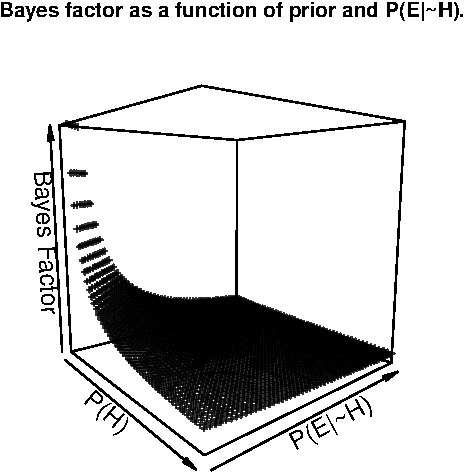
\includegraphics[width=1\linewidth]{lr-chapter4_files/figure-latex/fig-BayesFactorPrior-1} \end{center}
\caption{Impact of the prior and likelihood of E given ~H for probabilities in (0, 0.05) and Bayes Factor restricted to (0, 250) for visibility.}
\label{fig:BayesFactorPrior}
\end{figure}

A related reason to worry about the Bayes factor is pragmatic. Whoever
is tasked with assessing the strength of evidence---lay jurors, judges,
or expert witnesses who are offering their expertise to judges and lay
jurors---would face too great a cognitive burden. To see why, the
catch-all alternative hypothesis \(\neg H\) in the denominator
\(\pr{E}\) can be replaced by a more fine-grained set of alternatives,
\(H_1, H_2, \dots H_k\), provided \(H\) and these alternatives are
exclusive and cover the entire space of possibilities (that is, they
form a partition). So, the denominator \(\pr{E}\) should be unpacked, as
follows: \begin{align} \label{eq:lotpLong}
\pr{E} & = \pr{E\vert H}\pr{H} +\sum_{i=1}^k \pr{E\vert H_i}\pr{H_i}. 
\end{align}

\noindent Estimating \(\pr{E}\) now looks quite difficult. It would
require one to sift through the entire space of possibilities, as well
as coming up with a sensible selection of priors probabilities for the
several alternative hypotheses on hand.

A third reason to hesitate about the Bayes factor comes from an
observation by Gillies (1986), also discussed by Branden Fitelson
(1999). Consider the hypothesis \(H =\) ``the suspect is guilty'' and
suppose it is a fact that \(E =\) ``the suspect killed the victim.''
Fact \(E\) does not establish guilt with certainty since guilt requires
both \emph{actus reus}, the killing, and \emph{mens rea}, the intention.
But clearly \(E\) provides positive support for \(H\). Now consider a
composite hypothesis \(H'=\) ``the suspect is guilty \textit{and} we
live in a simulation built by aliens.'' Presumably, the support \(E\)
provides for \(H'\) should be weaker than the support it provides for
\(H\). After all, the addition of a far-fetched hypotheses should
decrease evidential support. This weakening of evidential support,
however, cannot be captured by the Bayes factor since both \(H\) and
\(H'\) deductively entail \(E\). In general, suppose \(H\models E\) (and
so, also, \(H \et X \models E\)). Then both \(\pr{E\vert H}\) and
\(\pr{E \vert H \et X}\) equal 1. But this means that
\(\mathsf{BF}(H,E) = \mathsf{BF}(H \et X, E) = \nicefrac{1}{\pr{E}}\).
So the Bayes factors for the two support relations are equal. This is
the problem of irrelevant conjuncts.\footnote{The same point can be made
  using irrelevant hypotheses that are not so far-fetched. For instance,
  suppose one hypothesis of interest is whether the victim was running
  in the park on a certain night, and the relevant piece of evidence is
  her footprints in the park. Perhaps, another hypothesis is whether she
  had wine at dinner later on. Clearly, whether she did is not obviously
  relevant to whether she was running in the park beforehand. However,
  one should be very hesitant to say that the evidential strength of the
  presence of footprints is the same relative to
  \emph{she was running in the park} and
  \emph{she was running in the park and had wine at dinner later on}.
  But this is what the Bayes factor would commit one to.}

So suppose we are after a measure of evidential stregth that (i) does
not depend on priors, (ii) places no unreasonably heavy cognitive
requirements, and (iii) is sensitive to the addition of irrelevant
conjuncts. We will argue that a measure that satisfies these desiderata
is the likelihood ratio, the ratio between \(\pr{E \vert H}\) (the
probability of the evidence given the hypothesis is true) and
\(\pr{E \vert \neg H}\) (the probability of the evidence given the
hypothesis is false). Before showing that this measure satisfies the
three desiderata, we address a preliminary questions. Why use such a
ratio in the first place?

For one thing, \(\pr{E \vert H}\) by itself would not be a fine-grained
enough measure. In some cases, this conditional probability may be close
to one. For instance, the probability that the blood type matches if the
accused is the source,
\(\pr{\textsf{blood match} \vert \textsf{source}}\), may be close to
one. Similarly, the probability that the DNA profile matches if the
accused is the source,
\(\pr{\textsf{DNA match} \vert \textsf{source}}\), may also be close to
one. But obviously a DNA match is not on par with a blood type match.
The DNA match should be stronger evidence that the blood type match
because a specific DNA profile occurs less frequently than a specific
blood type. And yet, a quantity such as \(\pr{E \vert H}\), by itself,
would fail to distinguish the two cases. Besides \(\pr{E \vert H}\),
also \(\pr{E \vert \neg H}\) matters. If the accused is \textit{not} the
source, the probability of a blood type match, while relatively small,
should be higher than the probability of a DNA profile match. Hence, the
likelihood ratio
\(\nicefrac{\pr{\textsf{DNA match} \vert \textsf{source}}}{\pr{\textsf{DNA match} \vert \neg \textsf{source}}}\)
should be higher than
\(\nicefrac{\pr{\textsf{blood match} \vert \textsf{source}}}{\pr{\textsf{blood match} \vert \neg \textsf{source}}}\).
This would explain why a DNA match is stronger evidence than a blood
type match.

Could the strength of evidence be measured by the probability
\(\pr{E \vert \neg H}\) alone? As before, relying solely on this
quantity would leave out crucial information. Consider an example by
Triggs \& Buckleton (2004). In a child abuse case, the prosecutor offers
\label{text:rock} evidence that a couple's child rocks and that only 3\%
of non-abused children rock,
\(\pr{\textsf{child rocks} \vert \neg \textsf{abuse}}=.3\). If it is
unlikely that a child who is not abused would rock, that this child
rocks might seem evidence of abuse. But this interpretation is mistaken.
It could also be that 3\% of abused children rock,
\(\pr{\textsf{child rocks} \vert \textsf{abuse}}=.3\). After all, the
two conditional probabilities need not add up to 1. Similarly, learning
that \(\pr{\textsf{child rocks} \vert \textsf{abuse}}=.3\) does not
provide enough information for evidence evaluation. One also needs
information about
\(\pr{\textsf{child rocks} \vert \neg \textsf{abuse}}\). If rocking is
equally unlikely under either hypothesis, rocking cannot count as
evidence of abuse. Neither of the two conditional probabilities, viewed
in isolation, makes this salient.

So, both the probability of the evidence given the hypothesis and the
probability of the evidence given an alternative hypothesis should be
part of any good measure of evidential strength (ENFSI, 2015; Royall,
1997; Triggs \& Buckleton, 2004). The Bayes factor includes both
probabilities, but---as seen before---it requires too much information
since it requires an assessment of the prior probability of the
hypothesis. A less demanding measure that that keeps track of both
probabilities is the \textbf{likelihood ratio}: \begin{align}
\label{eq:LR}
\tag{LR}
\mathsf{LR}(E,H,H') & = \frac{\pr{E \vert H}}{\pr{E \vert H'}},
\end{align}

\noindent where \(H'\) is a hypothesis that is taken to be a competing
alternative to \(H\). If the evidence is more likely given \(H\) than
\(H'\), the ratio would be above one, and if the evidence is more likely
given \(H'\) than \(H\), the ratio would be below one. As with the Bayes
factor, support levels correspond to deviations from one. The greater
the likelihood ratio (for values above one), the stronger the evidence
in favor of \(H\) as contrasted with \(H'\). The smaller the likelihood
ratio (for values below one), the stronger the evidence in favor of the
competing hypothesis \(H'\) as contrasted with \(H\).

Because of its simplicity, the likelihood ratio is sometimes used in
practice. Experts sometimes testify by offering the likelihood ratio as
a measure of the strength of the evidence. An expert, for instance, may
testify that the blood-staining on the jacket of the defendant is ten
times more likely to be seen if the wearer of the jacket hit the victim
(prosecutor's hypothesis) rather than if he did not (defense's
hypothesis) (CGG Aitken, Roberts, \& Jackson, 2010, p. 38). This
apparent simplicity, however, can often give rise to errors in the
assessment of the evidence, especially if the two hypotheses are not
chosen carefully. The choice of the hypotheses that are conditioned upon
is crucial. In the most straightforward case, \(H'\) is simply the
negation of \(H\). But the competing hypotheses \(H\) and \(H'\) need
not be one the negation of the other, a point to which we will return
later.

Let's now examine why the likelihood ratio satisfies our three
desiderata. First, unlike the Bayes factor, the likelihood ratio does
not depend on the prior probability of the hypothesis. It allows for a
clearer separation of the impact of the priors from the impact of the
evidence on the posterior probability. The relationship between
likelihood ratio \(\nicefrac{\pr{E \vert H}}{\pr{E \vert H'}}\), and
prior and posterior odds is apparent in the odds version of Bayes'
theorem: \begin{align}\label{eq:BTodds}
\frac{\pr{H \vert E}}{\pr{H' \vert E}}= \frac{\pr{E \vert H}}{\pr{E \vert H'}}\times \frac{\pr{H}}{\pr{H'}}.
\end{align} \noindent If the likelihood ratio is greater (lower) than
one, the posterior odds will be greater (lower) than the prior odds of
\(H\). The likelihood ratio, then, is a measure of the upward or
downward impact of the evidence on the prior odds of two hypotheses
\(H\) and \(H'\).

This feature of the likelihood ratio fits nicely with the division of
labor common in legal fact-finding between experts and decision-makers,
judges or lay jurors. A prominent forensic scientist recommends that `in
criminal adjudication, the values of the prior odds and the posterior
odds are matters for the judge and jury, in accordance with the normal
division of labor in forensic fact-finding' (Colin Aitken \& Taroni,
2008, p. 194). Experts should `not trespass on the province of the jury
by commenting directly on the accused's guilt or innocence, \dots and
should generally confine their testimony to presenting the likelihood of
their evidence under competing propositions' (CGG Aitken, Roberts, \&
Jackson, 2010, p. 42). If, however, experts were to report the Bayes
factor, this would mean they are competent to estimate \(\pr{E}\)
directly, which is unlikely, or that they implicitly estimate it relying
on their estimation of \(\pr{H}\) in the background (if they use the law
of total probability).

Second, the likelihood ratio is less cognitively burdensome than the
Bayes factor. It does not require one to think about the probability of
the evidence in general, \(\pr{E}\). Think, for example, of blood match
evidence. To calculate the Bayes factor, we need two things:
\(\pr{E\vert H}\) (which here, say, can be assumed to approximate one)
and \(\pr{E}\) (which is the probability of a blood match under any
possible scenarios, whether or not the the suspect is the source). Yet,
direct and reliable estimation of the probability \(\pr{E}\) is
difficult. One can use the law of total probability from equation
\eqref{eq:lotpSimple}. This would require, besides an assessment of the
conditional probabilities \(\pr{E\vert H}\) and \(\pr{E\vert \neg H}\),
an assessment of the prior probabilities of \(\pr{H}\) and
\(\pr{\neg H}\). Instead, the likelihood ratio would only require an
assessment of the conditional probabilities. In this sense, its
calculation requires less information.

Finally, unlike the Bayes factor, the likelihood ratio is not
susceptible to the problem of irrelevant hypotheses. For suppose
\(\pr{E\vert H} = \pr{E\vert H \et X} = 1\), where \(X\) is an
additional hypothesis that is irrelevant to \(H\). Note that
\(\mathsf{LR}(E,H) = \nicefrac{1}{\pr{E \vert \n H}}\), while
\(\mathsf{LR}(E, H \et X) = \nicefrac{1}{\pr{E \vert \n H \vee \n X}}\).
Unlike with the Bayes factor, here the two denominators might differ.
For example, suppose a fair coin is tossed three times. Let \(H=\) ``two
first tosses resulted in two heads,'' let \(E=\) ``at least one of the
two first tosses resulted in a head,'' and let \(X=\) ``the third toss
resulted in heads.'' Then \(\pr{E \vert H} =1\),
\(\pr{E\vert \n H} = \nicefrac{2}{3}\),
\(\mathsf{LR}(E,H) = \frac{1}{\nicefrac{2}{3}} = 1.5\). However,
\(\pr{E\vert H \et X} =1\), \(\pr{E \vert \n (H \et X)} \approx .71\),
so \(\mathsf{LR}(E,H \et X) \approx \frac{1}{.71} = 1.4\). Thus, the
support, as measured by likelihood ratio, can drop by adding a conjunct
that is probabilistically irrelevant to the original hypothesis. In
fact, this weakening of evidential support by adding an irrelevant
conjunct holds in general given sensible assumptions.\footnote{Branden
  Fitelson (2002) proved a general claim about irrelevant conjunctions.
  Hawthorne \& Fitelson (2004) later strengthened this claim. The claim
  is that, if \(\mathsf{LR}(E,H,\n H)>1\),
  \(\pr{E \vert X \et H} = \pr{E \vert H}\), and
  \(\pr{X \vert H} \neq 1\), then
  \(\mathsf{LR}(E,H,\n H) > \mathsf{LR}(E,H \et X,\n(H \et X))\). Crupi
  \& Tentori (2010) raised a related problem. They point out that if
  \(\mathsf{LR}(E,H)\leq 1\) and \(X\) is confirmationally irrelevant
  conjunct to \(H\) with regard to \(E\), then \(E\) will have the same
  negative or null impact on \(H \et X\), that is
  \(\mathsf{LR}(E,H \et X ) \leq \mathsf{LR}(E,H)\). They find this
  counter-intuitive and argue that this can be avoided by switching to
  the \(\mathsf{Z}\) confirmation measure (Crupi, Tentori, \& Gonzalez,
  2007). As we argue in Appendix \ref{sec:confirmation}, the
  \(\mathsf{Z}\) measure is prior-sensitive and therefore not fit for
  our purpose. Further, the phenomenon might not be deeply troubling
  either. If the likelihood ratio tracks how strongly the evidence
  supports a hypothesis, it should be no surprise that a more complex
  hypothesis---one obtained by adding an irrelevant
  proposition----enjoys a lower support from the same evidence.}

\vspace{1mm}
\footnotesize

\normalsize

All in all, the likelihood ratio outperforms the Bayes factor on several
respects. But, of course, there could be other measures of evidential
strength that fare even better. Other measures worth considering come
from the literature in formal epistemology on confirmation theory. The
expression `confirmation' is more commonly used in this literature
instead of strength of the evidence (or value, support). An extensive
discussion of these measures, however, would detract us from the main
task at hand, namely the examination of the pros and cons of the
likelihood ratio. We therefore relegate a discussion of confirmations
measures to Appendix \ref{sec:confirmation}. The upshot is that two
questions should be distinguished. (1) To what extend should a given
piece of evidence change our beliefs about a given hypothesis? Call this
the question about confirmation. (2) What is the strength of apiece of
evidence relative to a hypothesis? Call this the question about
evidential strength. The two questions overlap to some extent. The key
difference is that confirmation depends on prior probabilities, and
instead, in the evaluation of legal evidence in trial proceedings, the
assessment of evidential strength should preferably be kept separate
from the choice of prior probabilities. Confirmation measures are
concerned with (1) rather than (2), and thus they are unsuitable for
legal applications.

\hypertarget{the-risk-of-false-positive-and-its-impact}{%
\section{\texorpdfstring{The risk of false positive and its impact
\label{sec:fp}}{The risk of false positive and its impact }}\label{the-risk-of-false-positive-and-its-impact}}

The two conditional probabilities that make up the likelihood
ratio---\(\pr{E \vert H}\) and \(\pr{E \vert \neg H}\)---should be used
in the evaluation of any form of evidence, both quantitative and
non-quantitative evidence. This sections explore how DNA match evidence,
the most widely used form of quantitative evidence, should be evaluated
using the likelihood ratio. The argument formulated here can be
generalized to any form of `match evidence.' This evidence consists in a
statement by an expert that the defendant matches the physical material
found at the crime scene. The match can be between genetic profiles,
fingerprints, blood type, shoe prints, bite marks, etc.

Suppose an expert testifies that there is a genetic or DNA match between
the traces at the crime scene and a sample from the defendant. What is
this statement evidence for? It is evidence that the defendant was the
\textit{source} of the traces---that the materials found at the scene
originate from the defendant. The match can also be evidence that the
defendant was present at the scene or committed the act, but these
claims are more far-fetched, as the chain of inferences becomes weaker.
We will discuss these complications later in section
\ref{sec:lhTwoSTain}. For simplicity, let us focus on the source
hypothesis.

How strong is a DNA match \textit{qua} evidence that the defendant is
the source? Following the likelihood ratio, two conditional
probabilities should be compared here,
\(\pr{\textsf{match} \vert \textsf{source}}\) and
\(\pr{\textsf{match} \vert \neg \textsf{source}}\). When experts testify
in court about a DNA match, however, they only use the
\textbf{random match probability} as an indicator of evidential
strength. This is the probability that a random person, unrelated to the
crime, would coincidentally match the crime scene profile. The random
match can be equated to the probability that someone who is not the
source would match, \(\pr{\textsf{match} \vert \neg \textsf{source}}\).
This is one of the conditional probabilities in the likelihood ratio.
Should the other also be reported? In theory, it certainly should, but
in practice, it may not make a difference. The random match probability
is often an impressively low number, say 1 in 100 million, and alone can
be a good measure of evidential strength so long as the other
conditional probability, \(\pr{\textsf{match} \vert \textsf{source}}\),
is close to one. If that is the case, that
\(\pr{\textsf{match} \vert \neg \textsf{source}}\) is low would be
enough to ensure that the likelihood ratio is significantly above one.
But if

But this analysis---even assuming that
\(\pr{\textsf{match} \vert \textsf{source}}\) equals one---leaves out
other sources of error besides the random match probability. In
particular, equating the probability
\(\pr{\textsf{match} \vert \neg \textsf{source}}\) with the random match
probability neglects the risk of false positive matches, and this risk
is not negligible (Shaer, 2016). Note that a coincidental match is not
the same thing as a false positive match. For suppose two
individuals---say the perpetrator and the defendant---happen to share
the same DNA profile by coincidence. If an expert states that the crime
scene sample and the defendant's sample match, this would is a
coincidental match, but not a false positive match.

Unlike a coincidental match, a false positive match is often caused by a
human error in a number of circumstances (see W. C. Thompson, 2013 for a
more exhaustive treatment and multiple examples):

\raf{A: Bib references are missing here, is it on purpose?}

\begin{itemize}
\item
  \textbf{Cross-contamination of samples.} For instance, in Dwayne
  Johnson (2003) samples were accidentally swapped. In Lukis Anderson
  (2012), the genetic material was carried over by the paramedics. In
  one case, German police invested a considerable amount of time and
  effort searching for the so-called Phantom of Heilbronn, whose DNA
  profile was associated with many crimes. A bounty of 300k EUR was
  placed on her head. It turned out she was an innocent employee
  involved in the production of cotton swabs used across the country.
\item
  \textbf{Mislabeling of samples.} For instance, in 2011 the Las Vegas
  Metropolitan Police Department acknowledge that samples of two men
  suspected of a 2001 robbery were switched, leading to the exclusion of
  the perpetrator and four years of incarceration of the other suspect.
  The mistake came to light only because the perpetrator was later on
  arrested for an unrelated crime.
\item
  \textbf{Misinterpretation of test results.} Single-source sample
  comparison is not easily prone to misrepresentation, but evidence
  mixtures---often needed in sexual assault cases---are complicated to
  interpret. For example, Dror \& Hampikian (2011) re-examined a 2002
  Georgia rape trial in which two forensic scientists had concluded that
  the defendant could not be excluded as a contributor of the crime
  traces. The evidence was sent to 17 lab technicians for
  re-examination. One of them agreed that the defendant could not be
  excluded as a contributor. Twelve considered the DNA exclusionary, and
  four found it inconclusive. If the quantity of DNA is limited, there
  is uncertainty about the number of contributors and about whether any
  alleles are missing. Ultimately, there is an element of subjectivity
  in mixed DNA interpretation.
\end{itemize}

False positive DNA matches are not easy to detect for practical and
theoretical reasons. Since DNA evidence carries so much weight in court,
it is unusual to proceed with further DNA tests that are costly and
time-consuming. It is also unusual that a defendant or their family
could afford to pay for further DNA tests. Even more troubling is that
errors from contamination or mislabeling of samples often cannot be
detected with further DNA testing, because they will replicate the same
mis-identification. Sometimes, a lab discovers its own errors and
reports them, but this is rare (W. C. Thompson, 2013). Unfortunately, no
serious attempt has been made to systematically quantify the relevant
error rates. Anecdotal information suggest that false positive matches
take place more often than coincidental matches would entail, but how
often remains unclear (W. C. Thompson, 2013). Regular proficiency tests
used in accredited DNA laboratories involve comparison of samples from
known sources, but they are criticized for being unrealistically easy
(yet, it happens that analysts fail them). Sometimes, corrective action
files are made available. They usually show relatively few false
positive errors.\footnote{For instance, the Santa Clara County district
  attorney's crime laboratory between 2003 and 2007 caught 14 instances
  of evidence cross-contamination with staff DNA, three of contamination
  by unknown person, and six of DNA contamination from other samples,
  three cases of DNA sample switch, one mistake in which the analyst
  reported an incorrect result, and three errors in the computation of
  the statistics to be reported.} But because of the fragmentary
information available, it would be premature to conclude that these
errors are no cause for concern.

We should now incorporate the risk of false positive matches into a more
adequate assessment of the strength of a DNA match. This can be done
using the likelihood ratio, following Colin Aitken, Taroni, \& Thompson
(2003). We abbreviate:

\begin{center} \hspace{10mm}
\begin{tabular}{lp{9cm}}
$S$ & The specimen comes from the suspect (source). \\
$R$ & A match is reported (reported match). \\
$M$ & There is a true match (true match).
\end{tabular}
\end{center}

\noindent The difference between \(S\) and \(M\) is that a true match
will exist not only if the suspect is the source, but also if, even
though the defendant is not the source, the profiles are in fact the
same due to a random, coincidental match. Similarly, a reported match
might arise not only if there is a true match, but also if a false
positive error has been made. These possibilities are represented in
Figure \ref{fig:fpp}.

\begin{center}
\begin{figure}
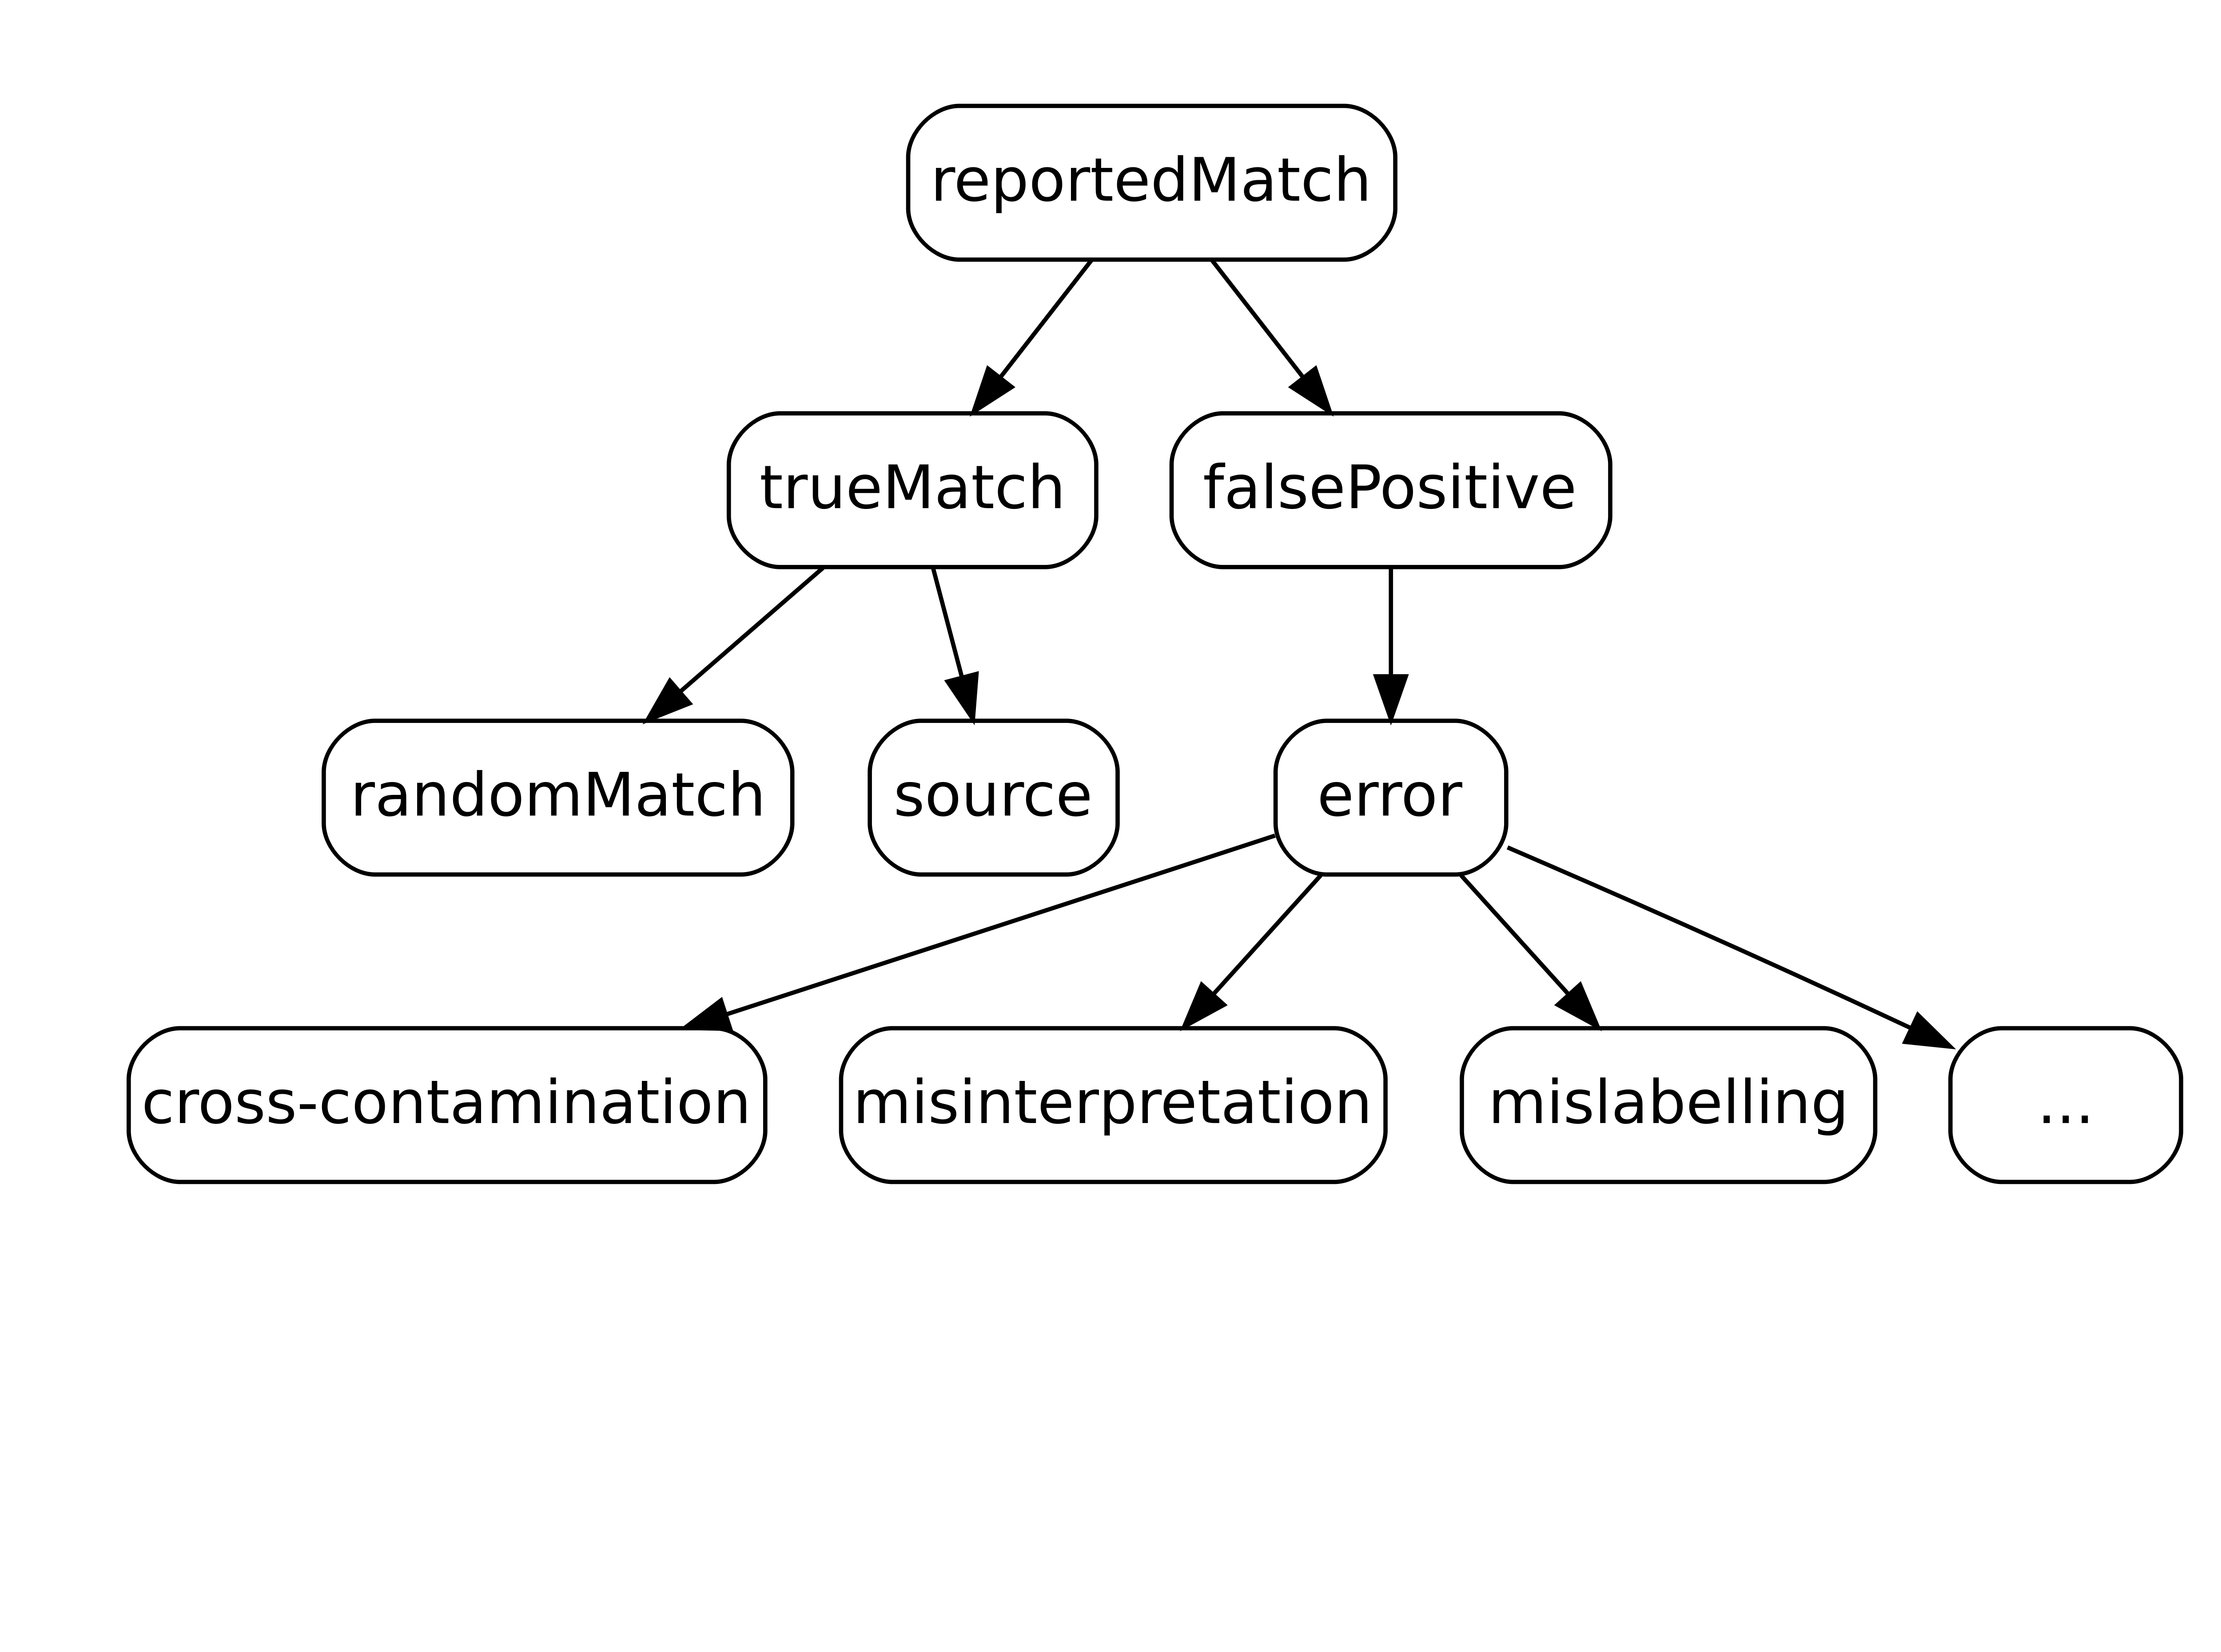
\includegraphics[width = 12cm]{img/fpp.png}
\caption{Dependencies between variables in the false positive problem.}
\label{fig:fpp}
\end{figure}
\end{center}

The evidence whose strength should be assessed is the \textit{reported}
match relative to the pair of hypotheses \(S\) and \(\neg S\). So the
likelihood ratio should have the form:
\(\nicefrac{\pr{R \vert S}}{\pr{R \vert \neg S}}\). Taking the risk of
false positive matches into account, the likelihood ratio can be written
as:

\begin{align}
\label{eq:LRfp4}
\frac{\pr{R \vert S}}{\pr{R \vert \neg S}} & = \frac{1}{\pr{R \vert  M}\pr{ M \vert \n S} + \pr{R \vert \n M}\pr{\n M \vert \n S}}\\
& = \frac{1}{RMP + [ FPP \times (1-RMP)]}
\end{align}

\noindent The expression RMP stands for the random match probability
\(\pr{M\vert \n S}\) and the expression FPP stands for the false
positive probability \(\pr{R \vert \n M}\). This should highlight the
difference between the two error probabilities. A false positive
probability tracks a human error, the possibility that match may be
reported (\(R\)) even without a true match (\(\neg M\)). The random
match probability, instead, tracks a coincidence of nature---the
possibility that someone who is not the source (\(\neg S\)) could still
be---coincidentally---a true match (\(M\)). The denominator mirrors the
fact that there are two ways misleading evidence can arise: there is a
true match and the suspect is not the source (because of a random,
coincidental match), or there is no true match, and an a false positive
error has been made in the identification process. The numerator
simplifies to one because the probability of a false negative is assumed
to be one. We will relax this assumption later one. The full derivation
is given below. The reader may skip it without loss to the overall
argument.

By the law of total probability, the denominator \(\pr{R \vert \neg S}\)
can be unpacked as
\(\pr{R \wedge M \vert \neg S} + \pr{R \wedge \neg M | \neg S}\). The
latter, by the chain rule, is equivalent to
\(\pr{R \vert M \wedge \neg S}\pr{ M \vert \n S} + \pr{R \vert \n M \wedge \neg S}\pr{\n M \vert \n S}\).
A similar reasoning applies to the numerator. The likelihood ratio then
becomes:

\begin{align}
\frac{\pr{R \vert S}}{\pr{R \vert \neg S}} & = \frac{\pr{R \vert M \et S}\pr{M \vert S} + \pr{R \vert \n M \et S}\pr{\n M \vert S}}
{\pr{R \vert M \et \n S}\pr{M \vert \n S} + \pr{R \vert \n M \et \n S}\pr{\n M \vert \n S}}
\end{align}

\noindent This expression can be simplified by assuming that a reported
match (\(R\)), assuming a true match obtains (\(M\)), is independent of
whether the suspect is the source (\(S\)): \begin{align}
\label{eq:indOnS}
\pr{R \vert M \et S} & = \pr{R \vert M \et \n S} = \pr{R \vert M}
\\ \nonumber
\pr{R \vert \n M \et S} & = \pr{R \vert\n M \et \n S} = \pr{R \vert \n M},
\end{align}

\noindent Now, apply \eqref{eq:indOnS} in four places: \begin{align}
\label{eq:LRfp2}
\frac{\pr{R \vert S}}{\pr{R \vert \neg S}} & = \frac{
\pr{R \vert M}\pr{M \vert S} + \pr{R \vert \n M}\pr{\n M \vert S}
}{
\pr{R \vert M }\pr{M \vert \n S} +
\pr{R \vert \n M}\pr{\n M \vert \n S}
}
\end{align}

\noindent In addition, for simplicity, take the probability of a false
negative to be zero. We will consider the case in which it is not zero
later on. In fact, the reasons for taking false positives seriously are
also reasons for taking false negatives seriously, but let's deal with
one problem at a time. So, let the probability of a true match if the
suspect is a source be one: \begin{align}
\label{eq:ifSthenM}
\pr{M\vert S} = 1  \,\,\, \mbox{ so also } \,\,\, \pr{\n M \vert S}=0,
\end{align} \noindent and let the probability that a true match is
reported also be one: \begin{align}
\label{eq:fnNull}
\pr{R \vert M} & = 1.
\end{align}

\noindent Finally, using \eqref{eq:ifSthenM} and \eqref{eq:fnNull} in
the numerator yields the desired formula:

\begin{align}
\frac{\pr{R \vert S}}{\pr{R \vert \neg S}} & = \frac{1}
{\pr{R \vert  M}\pr{ M \vert \n S} + \pr{R \vert \n M}\pr{\n M \vert \n S}}
\end{align}

Figure \ref{fig:fpplr} shows the impact of the probability of a false
positive match (between 0 and 0.05 probability) assuming random match
probabilities in the order of \(10^{-9}\) (often reported in the case of
two single-source samples over ten or more loci) and \(10{^-3}\)
(sometimes obtained by means of less discriminating tests when the
comparison involves a mixed sample). Even a small increase in the false
positive probability can lower the likelihood ratio dramatically.

\begin{figure}

\begin{center}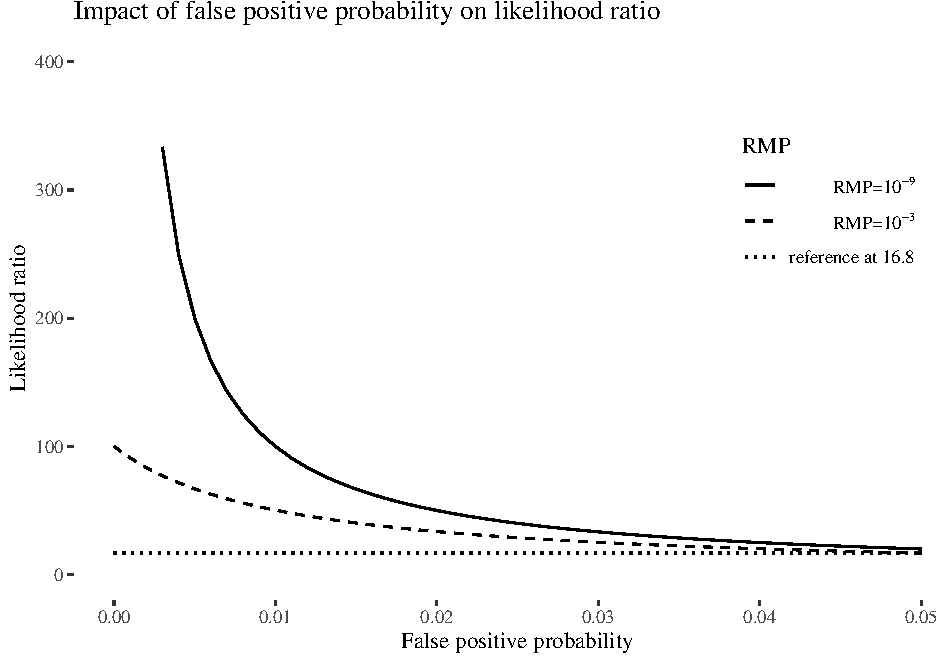
\includegraphics[width=1\linewidth]{lr-chapter4_files/figure-latex/fig-fpplr-1} \end{center}
\caption{Impact of the false positive probability on the likelihood ratio for two values of RMP. The horizontal reference line is at 16.8, the likelihood reached at RMP=$10{^-3}$ for FPP=0.05. At the same value of FPP, the LR for RMP $10{^-9}$ is 20.}
\label{fig:fpplr}
\end{figure}

\todo{The rest of this section needs rewriting}

We have not yet considered the possibility of false negative matches.
The formula for the likelihood ratio should inclide this possibility.
This can be done quite easily.

\begin{align}
\frac{\pr{R \vert S}}{\pr{R \vert \neg S}} & = \frac{\pr{R \vert M}\pr{M \vert S} + \pr{R \vert \n M}\pr{\n M \vert S}}{\pr{R \vert M }\pr{M \vert \n S} + \pr{R \vert \n M}\pr{\n M \vert \n S}}\\
& = \frac{1-FPP}{(1-FPP)RMP + [ FPP \times (1-RMP)]}
\end{align}

Buckleton, Bright, \& Taylor (2018) derive a more general formula for
the likelihood ratio. First, they make the conceptual distinction
between the probability that an error occurs (\(E\)) and the probability
that a match is reported if it does. Mind your head: here \(E\) stands
for error, not for evidence! In terms of our notation, we have:
\begin{align*}
e & = \pr{E} = \pr{E \vert S} = \pr{E \vert \n S}
\end{align*} \noindent That is, we denote the probability of error as
\(e\), and we assume it doesn't depend on whether the prosecution
hypothesis is true (whether the suspect is the source).

Separately, the formula includes the probability of a reported match if
an error occurs, also assumed to be independent of whether the
prosecution hypothesis is true: \begin{align*}
k =  \pr{R \vert E, S} = \pr{R \vert E, \n S}
\end{align*} \noindent Further, it is assumed that the probability of
false negatives is zero (\(\pr{R \vert S, \n E} =1\)) and the
probability of reported match if no error occurs and the defense
hypothesis is true is RMP (\(\pr{R \vert \n E, \n S}=RMP\)).

Now the derivation: \begin{align*}
LR & = \frac{\pr{R\vert S}}
{\pr{R \vert \n S}}\\
& = \frac{\pr{R \vert \n E, S}\pr{\n E \vert S} + \pr{R \vert E, S}\pr{E \vert S}}
{\pr{R \vert \n E, \n S}\pr {\n E \vert \n S} + \pr{R \vert E, \n S}\pr{E \vert \n S}}\\
& = \frac{1(1-e) + ke}
{RMP(1-e)+ke}  = \frac{1-e+ke}{RMP  - e\times RMP + ke} \\
& = \frac{1 - (1-k)e}{RMP(1-e)+ke}
\end{align*}

Let's take it slow. First, the likelihood ratio is just the ratio of
probabilities of a reported match (1) if the suspect is the source and
(2) if the suspect is not the source.

Now, think of \(\pr{R\vert S}\). This can be split into two possible
scenarios: an error has not been made, or an error has been made.
Accordingly, the numerator in the second line uses the law of total
probability to split \(\pr{R\vert S}\) into these two options.

Similarly, \(\pr{R\vert \n S}\) can be split into two cases: the suspect
is not the source, but we are dealing with a random match, or the
suspect is not the source, and an error has been made. An application of
the law of total probability in the denominator mirrors this. The rest
of the argument is just rewriting in terms of abbreviations, and
algebraic manipulation.

Note now that if you think of an error as something that guarantees a
mistaken identification, \(k\) becomes \(1\) and \(e\) becomes the false
positive rate. On this assumption straightforward algebraic manipulation
gives: \begin{align*}
 \frac{1 - (1-k)e}{RMP(1-e)+ke} & = \frac{1-e+e}{RMP(1-e)+e}\\
 & = \frac{1}{RMP - e\times RMP + e} = \frac{1}{1 + e(1-RMP)}
\end{align*} \noindent which is the same as the formula obtained by
Colin Aitken, Taroni, \& Thompson (2003) if we take \(e\) to be FPP, as
we should on the assumption that \(k=1\).

An analogous reasoning can be used to study the impact of false negative
probability on the value of exculpatory DNA evidence. Consider the
probability of no match being reported if an error has been made,
analogous to \(k\) above: \begin{align*}
l & = \pr{\n R \vert E, S} = \pr{\n R \vert E, \n S} = \pr{\n R\vert E}
\end{align*} \noindent Now, the likelihood ratio calculations, assuming
\(l = 1\), go as follows:

\begin{align*}
\mathsf{LR}(\n R, S, \n S) & = \frac{\pr{\n R \vert S}}{\pr{\n R \vert \n S}} \\
& = \frac{\pr{\n R \vert \n E, S}\pr{\n E \vert S} + \pr{\n R \vert E, S}\pr{E \vert S}}
{\pr{\n R \vert \n E, \n S}\pr{\n E \vert \n S} + \pr{\n R \vert E,\n S}\pr{E \vert \n S}} \\
& = \frac{0 (1-e) +  le}
{(1-RMP)(1-e) + le} \\
& = \frac{le}
{1- RMP - e + eRMP + le} = \frac{le}{1-RMP + e(l + RMP -1)}\\
& = \frac{e}{1 - RMP + eRMP} = \frac{e}{1+(e-1)RMP}
\end{align*}

\noindent If the error rate is 0, then the numerator is 0 and so is the
\textsf{LR}, as it should. In such a case, the evidence is completely
exculpatory, the posterior probability that the suspect is the source
will be also 0. If the error rate is not 0, the numerator simply is the
probability of error, and the numerator takes values between \(1-RMP\)
and \(1\), depending on the value of \(e\). Quite crucially, 1 in the
denominator is decreased by \((1-e)RMP\), which with usually very low
RMP in the case of DNA evidence is a very small change as compared to
one, so the denominator stays very close to 1 even if \(e\) is very
high, and the \textsf{LR} effectively simply is
\(\approx \nicefrac{e}{1} = e\). The lines in Figure \ref{fig:fnplr},
strictly speaking, do not overlap, but the difference between them (with
\(RMP\) being fairly low) is negligible.

\begin{figure}

\begin{center}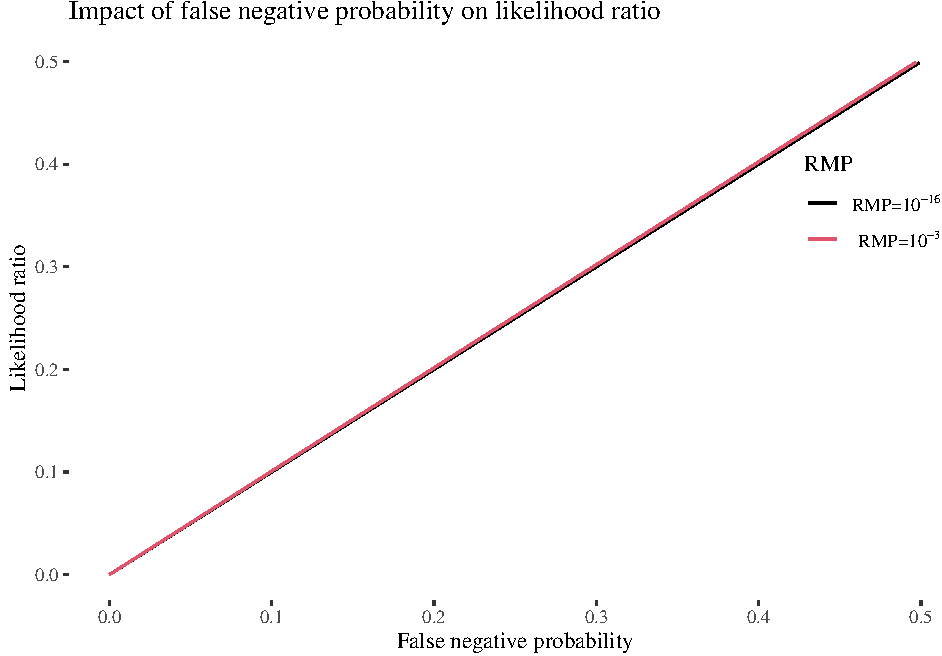
\includegraphics[width=1\linewidth]{lr-chapter4_files/figure-latex/fig-fnplr-1} \end{center}
\label{fig:fnplr}
\caption{Impact of the false negative probability on the likelihood ratio of exculpatory evidence for two values of RMP.}
\end{figure}

Interestingly, there is a sense in which the situation is not symmetric
when we compare FPP to FNP. With FPP, the LR is 50 when \(e=0.01\) for
RMP\(=10^{-3}\), while for the same \(e\) and RMP it is \(0.01\) for
FNP, an hundredfold decrease. This illustrates that the exculpatory
value of DNA evidence is higher than its incriminating value, even if
the error rates and random match probabilities are the same.

Some conceptual symmetry can be regained though. Suppose \(RMP\) is
really low as compared to \(FPP\) and let's ignore it in our
approximation. Then, the likelihood ratio of the incriminating evidence
becomes \(\nicefrac{1}{FPP}\) and the likelihood ratio of exculpatory
evidence becomes \(\nicefrac{FNP}{1}\). However, the change rate of
these differ. While
\(\nicefrac{d}{dx}(\nicefrac{1}{x}) = \nicefrac{d}{dx} (x^{-1}) = - \nicefrac{1}{x^2}\),
\(\nicefrac{d}{dx}(\nicefrac{x}{1})=1\), and the derivatives look quite
different (Figure \ref{fig:der})

\begin{figure}[h]

\begin{center}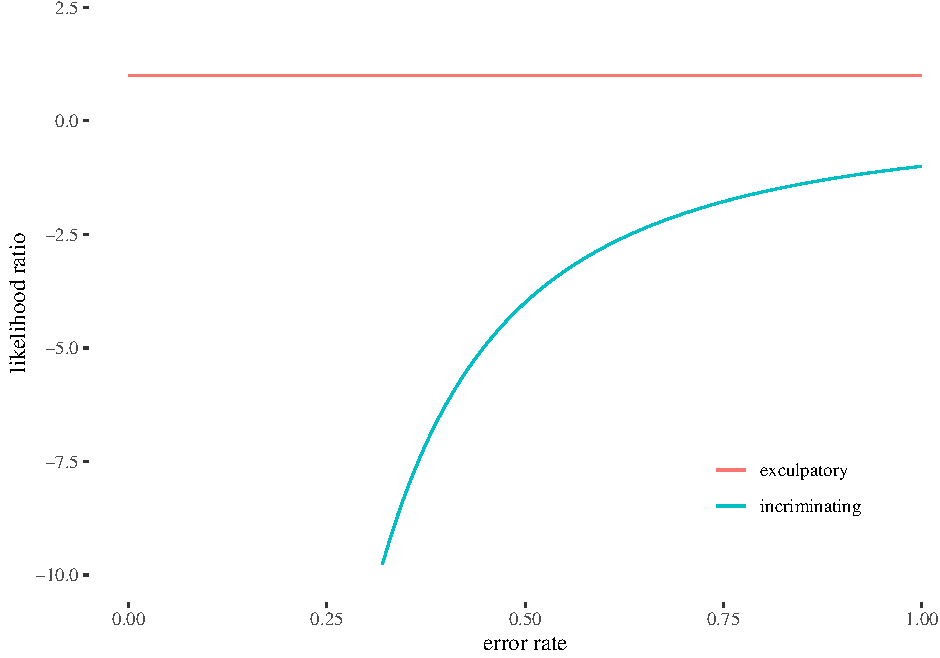
\includegraphics[width=1\linewidth]{lr-chapter4_files/figure-latex/fp-derivatives-1} \end{center}
\caption{Derivatives of incriminatory and exculpatory likelihood ratios, range restricted to (-10,2).}
\label{fig:der}
\end{figure}

The key lesson from this section is as follows. First, likelihood ratios
are useful in the evaluation and comparison of the impact of positive an
negative error rates: and it makes clear that this impact is not the
same, contrary to what one may intuitively think. Second, the likelihood
ratio analysis reveals that even a seemingly small error rate in a sense
trumps random match probability: if you think there are good reasons to
worry about random matches, the analysis shows that there are much
better reasons to worry about error rates. While in fact error rates
have not been properly studied, the above application of likelihood
ratio to investigate the potential impact of hypothetical error rates is
still useful in guiding further research, as it clearly suggests that
error rates may have serious impact on the value of various types of
evidence, and so require attention.

\hypertarget{eyewitness-identification-and-likelihood-ratio}{%
\section{\texorpdfstring{Eyewitness identification and likelihood ratio
\label{sec:eyewitness}}{Eyewitness identification and likelihood ratio }}\label{eyewitness-identification-and-likelihood-ratio}}

So far we paid attention to DNA evidence, a form of quantitative
evidence widely used in trial proceedings. But the question arises
whether evidence that is not explicitly quantitative, for example,
eyewitness testimony, can also be evaluated using likelihood ratio. We
show that the answer is affirmative. In fact, there is no sharp divide
between quantitative and non-quantitative evidence. The statement that
the crime scene DNA matches the defendant's DNA is qualitative, but its
value is best assessed by means of numerical information, such as error
rates and the random match probability. Similarly, a witness testifying
`I saw him!' carries a lot of weight in a court of law, but again, its
value is best assessed by means of numerical information, such as data
about the risks of false identifications. These risks should not be
downplayed nor exaggerated. As we will show, quantitative information
can be used to this effect and can be combined in a principled manner
into the likelihood ratio.

To start, there is plenty of quantitative information about the risks of
false eyewitness identifications. Consider first statistics about false
convictions. The rate of false convictions in death penalty cases in the
United States is estimated at about 4\% (Gross, O'Brien, Hu, \& Kennedy,
2014). How much can be attributed to false eyewitness identifications is
hard to say exactly, but presumably quite a bit. In fact, a study of 340
exoneration in the years 1989-2003 shows that around 90\% of false
convictions in rape cases resulted from a false eyewitness
identification. This percentage comes close to 100\% in rape convictions
in which the victim and the defendant were of difference races. In
murder cases, 43\% of false convictions resulted from a false
identification by one or multiple eyewitnesses. \todo{REFERENCE MISSING}

Field studies offer an equally discouraging picture. These studies show
that, in line-up identifications, eyewitnesses select filler individuals
at a rate of 20-24\% (Klobuchar, Steblay, \& Caligiuri, 2006) . That is,
around 20\% of the time, an innocent person in a police line-up is
incorrectly identified as the perpetrator. Similarly, a field study in
Greater London (Wright \& McDaid, 1996) and another study in Sacramento,
California (Behrman \& Davey, 2001) indicate that the false
identification rate is around 20\%. Even in experimental
settings---where witnesses are less emotionally taxed---eyewitnesses
identify a filler indiividual from a line-up in approximately 20\% of
the cases (S. G. Thompson, 2007).

In light of these empirical results and similar studies, the justice
systems has grown suspicious of eyewitness evidence over the last twenty
years. This skepticism is welcome but should not lead to discounting
relevant evidence. Some may caution that the risks of mistaken
identification should be assessed in the individual circumstances, and
that blanketed statements that eyewitnesses are unreliable---even when
backed up by well-researched statistics---are not very helpful. After
all, judges and jurors should make determinations about the reliability
of a specific eyewitness identification, not about eyewitness
reliability in general. Cross-examination is often thought to be the
tool for this individualized assessment of the risk of error.\footnote{The
  evidence law scholars Henry Wigmore in his monumental treatise on the
  law of evidence famously asserted that `cross-examination is greatest
  legal engine ever invented for the discovery of truth.' This assertion
  has been subject to little empirical testing.}
\todo{reference missing} Unfortunately, empirical studies suggest that
cross-examination is ineffective at detecting false identifications. In
a series of experiments, subjects were asked to cross-examine
eyewitnesses to determine whether witnesses made accurate or mistaken
identifications. Subjects showed little or no ability to make such
discrimination (Wells \& Olson, 2003, p. 285). In another experiment, a
representative sample of \(48\) witnesses was cross-examined. Subjects
(\(n = 96\)) viewing the cross-examinations showed little ability to
distinguish accurate from false identifications (Lindsay, Wells, \&
Rumpel, 1981).

The ineffectiveness of cross-examination at detecting a false
identification might stem from its reliance on intuitive, folk
assessment of the risks of error, not on well-researched quantitative
data. The research on eyewitness testimony can improve this state of
affairs since a great deal of it aims to identify the conditions under
which an identification goes awry. These conditions are usually divided
into system variables and estimator variables (Behrman \& Davey, 2001;
Wells \& Olson, 2003) . The former refer to how the identification took
place in a regimented setting, say whether it was a line-up or a
showup;\footnote{A showup refers to the observation of a single suspect by a witness in the field, typically at the crime scene. A lineup refers to the presentation of the suspect and several foils, either live or via photographs.}
whether the line-up was simultaneous or sequential; whether the witness
identified a suspect prior to the line-up; etc. Estimator variables,
instead, refer to the environmental conditions. These variables include
distance, lighting conditions, time, the presence of a weapon, etc.

An additional factor to consider is the confidence of the witness in the
identification. It is a point of contention whether or not confidence is
positively correlated with an accurate identification. A meta-analysis
by Wixted \& Wells (2017) offers a nuanced but overall optimistic
picture. Their analysis focuses on identifications under
\emph{pristine conditions}. They require, for example, a double-blind
line-up containing one suspect and at least five fillers with no
resemblance to the suspect. The witness is cautioned that the offender
might not be in the line-up and there is no expectation that they
identify someone. Needless to say, very few police departments run their
lineups in pristine conditions. But, as it turns out, if the
identification occurs under pristine conditions, the high confidence of
the witness in the identification is strongly predictive of an accurate
identification. Most interestingly, witnesses with high confidence under
pristine conditions should be around 90\% accurate, a rather encouraging
figure.\footnote{The extent to which initial high confidence under
  pristine conditions is indicative of accuracy depends on the base rate
  of target-present lineups. In lab studies the base rate is about 50\%,
  but in real-life circumstances, the best estimate is about 35\%.}

So, a more individualized assessment of the risks of false eyewitness
identification can be made by taking into account estimator and system
variables, as well as other relevant factors such as eyewitness
confidence. Cross-examination serves a similar purpose. Questions about
time of day, distance, stress level, etc. elicit information about
estimator variable as well as system variables. Empirical research on
eyewitness testimony can supply numerical information about the
significance of these variables. It can help to answer questions such
as, how much does poor visibility or distance increase the risk of a
false identification? Ideally, properly formatted data about all the
factors we discussed could be used to develop a multivariate model. This
model would allow an assessment of the risks of a false identification
under a variety of relatively well-specified circumstances elicited
during cross-examination. We are far from reaching this state of
maturity, but even with the current research, an expert who is aware of
the literature we have cited and of the specific circumstances of the
case could assess the risks of a false identification quantitatively. An
untrained jury member unaided by numerical data---even after
cross-examination---is unlikely to arrive at a better assessment of the
risks of error involved.

So consider two scenarios in which we numerically estimate the
reliability of the eyewitness evidence in line with the research we just
discussed. In one, such an expert recognizes the identification
conditions as pristine and testifies: the probability of the testimony
if the suspect in fact is the perpetrator (\(\pr{E\vert H}\)) is
\(.9\% \pm .05\), and the false positive probability
(\(\pr{E \vert \n H}\)) is \(.1\pm .03\). In scenario two, the
conditions were not pristine, and the expert testifies that
\(\pr{E\vert H}=.8 \pm .05\) and \(\pr{E\vert \n H}=.25 \pm .05\). We
get two different \emph{ranges} of likelihood ratios, \(lr_1\) and
\(lr_2\). In the first case, the minimum and the maximum are as follows:
\begin{align*}
\mathsf{min}(lr_1) = \nicefrac{.95}{.07} \approx 13.57  & \,\,\,\,\,\,\,\,  \mathsf{max}(lr_1) = \nicefrac{.85}{.13} \approx 6.53  
\end{align*} \noindent so the expert can, say, testify that the
likelihood ratio is in the range of 6.5-13.5. In the second scenario,
the minimum and the maximum are as follows: \begin{align*}
\mathsf{min}(lr_1) = \nicefrac{.85}{.2} =  4.25 &  \,\,\,\,\,\,\,\,   \mathsf{max}(lr_1) = \nicefrac{.75}{.3} \approx 2.5  
\end{align*} \noindent so the expert can testify that the likelihood
ratio is in the range of 2.5-4.25.

Now, suppose further evidence is put forward to the effect that the
suspect blood type matches the crime scene sample. Say the probability
of a match if the suspect is the source is simply 1, while the
probability of a random match is .05. The likelihood of this evidence
alone is \(\nicefrac{1}{.05}= 20\). Assuming independence, the joint
likelihood for total evidence is obtained by multiplying separate
likelihood ratios. Now, without any commitment to the priors, the impact
of likelihood ratio ranges on any prior probability can be quantified
and visualized, as in Figure \ref{fig:eyewitness3}.

\begin{figure}[h]

\begin{center}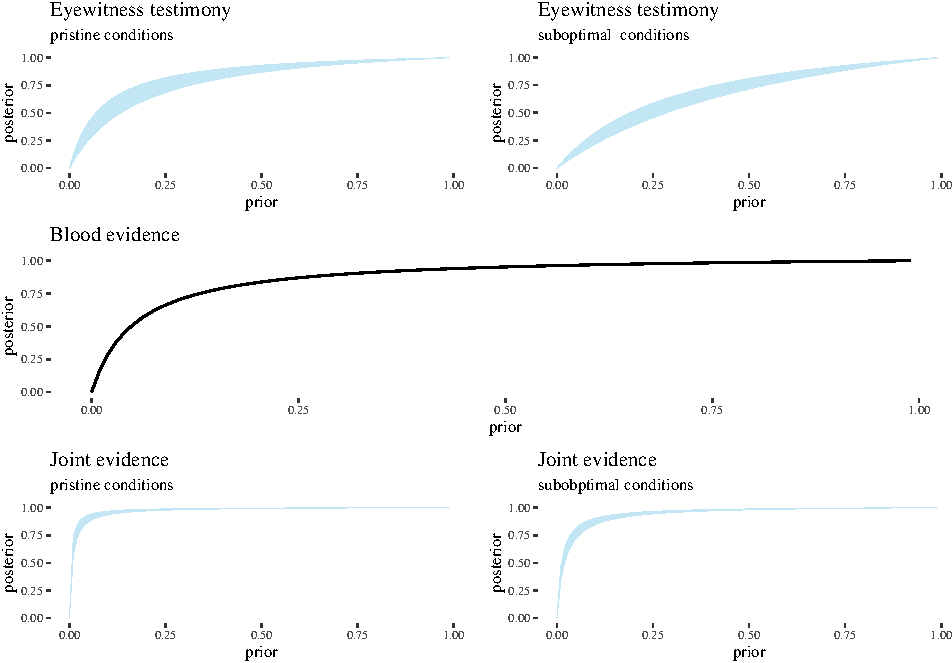
\includegraphics[width=1\linewidth]{lr-chapter4_files/figure-latex/eyewitness2-1} \end{center}
\caption{Impact of converging items of  evidence on the posteriors.}
\label{fig:eyewitness3}
\end{figure}

What about conflicting evidence? Suppose this time the conditions were
pristine, the expert's evaluation of the eyewitness evidence in pristine
conditions is as before, but the witness identified someone else than
the suspect (evidence \(E\)), while DNA evidence (evidence \(D\))
supports the prosecution hypothesis \(H\) with \textsf{LR} = 300 (this
is, say, because we take the false positive probability seriously).
Then, the range of plausible likelihood ratios for eyewitness evidence
alone is:

\begin{align*}
\left[\frac{.07}{.95}, \frac{.13}{.85}    \right ]  & \approx [.073,.15]
\end{align*}

In contrast, if the eyewitness is a friend of the suspect, so that you
estimate \(\pr{E \vert H}\) to be .6, while the conditions were
sub-optimal, so that \(\pr{E\vert \n H} = .8\pm .05\), the likelihood
ratio range is \(.7-.8\) and the impact of such eyewitness evidence is
quite different.

\vspace{1mm}
\footnotesize

\normalsize

\begin{figure}[h]

\begin{center}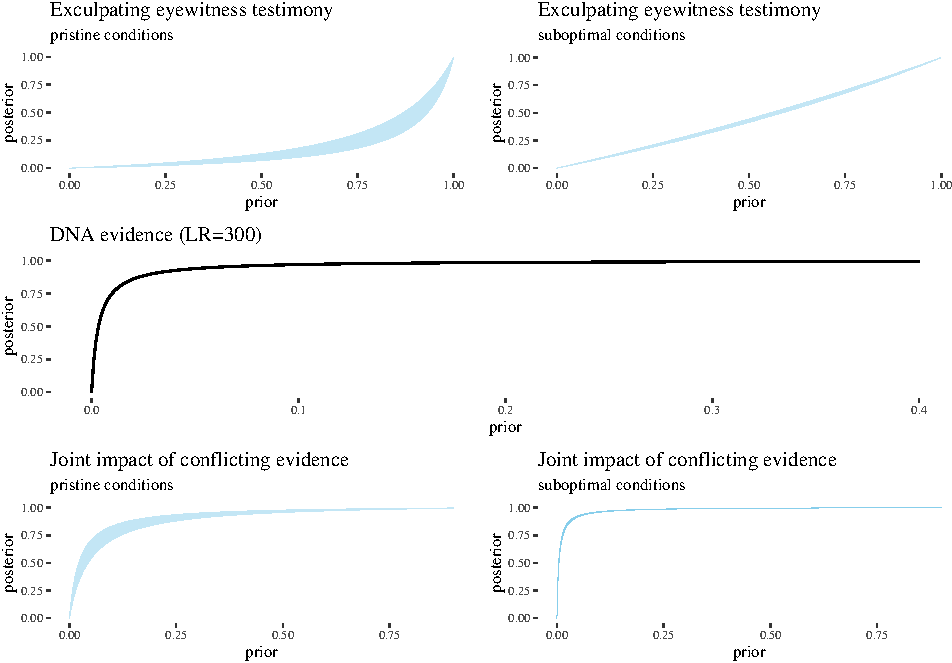
\includegraphics[width=1\linewidth]{lr-chapter4_files/figure-latex/eyewitness4-1} \end{center}
\caption{Impact of conflicting items of  evidence on the posteriors.}
\label{fig:eyewitness4}
\end{figure}

The key observation here is that whether exculpatory eyewitness
testimony can in fact be sufficient to acquit in light of incriminating
DNA evidence depends on the particulars: both on the quality of the
eyewitness testimony and on the realistic assessment of the likelihood
ratio for the DNA evidence (incorporating the probability of false
positives), and on what priors other pieces of evidence led us to so far
prior to the evaluation of such items of evidence. The devil is in the
detail, and it is not always the case that one should trump the other.

The reader might be disappointed: simply saying ``it depends'' does not
seem to help much. However, keep in mind that there are well known items
in the literature, on one hand, in psychology, illustrating that human
jurors tend to value eyewitness evidence over statistical evidence
(Niedermeier, Kerr, \& Messeé, 1999; Wells, 1992; Wells \& Olson, 2003),
and, on the other hand, in epistemology, attempting to explain this
intuition in a philosophically principled manner (Bolinger, 2020; Smith,
2017; Thomson,
1986).\mar{R: try to come up with  more references in this passage, think about this.}
In line with a more balanced view (Redmayne, 2008), our approach
suggests that while the psychological effect exists, there are multiple
cases in which the preference for eyewitness evidence is mistaken, and
relegates the identification and evaluation of factors that contribute
to its proper evaluation to actual empirical research. If the situation
is complicated, the best that can be done is take its complexity
seriously, and quantitative methods are much more fit for this task than
juror's intuitions or general philosophical statements.

Here is an example of real-life complexities that the considerations in
this section can clarify to some extent. In
\emph{The People of the State of New York v. Bansheen Rush} (Supreme
Court of New York, 1995), a rape victim identified the defendant from
photographic a few weeks after the event, identified the defendant in a
corporeal lineup two weeks later, but at trial identified a spectator as
her assailant, so the previous identifying evidence has been
precluded.\footnote{Interestingly, Articles 60.25 and 60.30 of the \emph{Rules of Evidence and Related Matters} referred to at this point by the court do not say anything about mixed eyewitness evidence of this sort: they only define eyewitness evidence as requiring recognition after the event in a proper  procedure (not at trial).}
The defendant had been seen in the vicinity of the crime location three
days before the crime. A DNA expert provided a positive match and
testified that the random match probability is 1 in 500 million. The
court found the DNA evidence alone to legally sufficient to support the
guilty verdict.

In light of our discussion so far, this deserves a few remarks. First,
the circumstances of the first two are not described in sufficient
detail to decide how the existing research applies. To correctly deploy
the results, information would be needed on how much the two first
identification conditions departed from pristine conditions and in what
respects. Moreover, it is known that the quality of testimony decreases
with time, and is even less reliable in a stressful situation such as
the trial. So, overall, the three testimonies jointly still constituted
positive identifying evidence, albeit weakened by the mistake (made in
the most stressful conditions and with much more time between the crime
and the identification), but without further details, it is hard to
judge the extent or estimate the joint reliability quantitatively.
Second, while the random match probability has been fairly low, some
doubts remain as no estimates of false positive probability are
available, and so it is difficult to estimate its impact on the final
likelihood ratio of the DNA evidence.

Again, this might be disappointing, if the reader expected a precise
numerical evaluation. However, this is still far from useless: it
suggests that the eyewitness evidence preclusion was over-cautions, that
more attention should have been paid to the detailed circumstances of
the first two identifications, and that more reliable research is needed
on false positive probabilities in DNA identifications for such cases to
facilitate the handling of such unusual cases. If these elements had
been in place, one could, in principle, be more specific about the value
of the joint evidence.

The discussion in this section points towards an approach that we will
be developing in other chapters.\(\,\)\todo{crossref} The evaluation of
eyewitness testimony turns out to be quite complicated and depends on
various factors. This multivariate nature of the problem makes Bayesian
networks a plausible tool for the representation of the factors at play
and for the assessment of how they interact. Moreover, eyewitness
evidence is often subject to cross-examination. While in general it is
meant to elicit further information that would change the evaluation of
the evidence, there are a few different ways the situation might
develop, and several argumentative moves that can be made in such a
context. On one hand, the additional evidence obtained can
\textbf{rebutt} the eyewitness evidence, if it supports a hypothesis
incompatible with the original one, as might happen when the eyewitness
makes a statement contradicting something they have said previously. On
the other, the new evidence might \textbf{udercut} the eyewitness
testimony if it leads to the re-evaluation of the witness's reliability
without leading to a new hypothesis, as might happen when the eyewitness
provides new evidence about the lightning conditions. Such moves, again,
can be suitably modeled in terms of Bayesian networks (Di Bello, 2021).
Here we just mention this connection to Bayesian networks, and it will
be explored more extensively later on.

\hypertarget{hypothesis-choice}{%
\section{\texorpdfstring{Hypothesis choice
\label{sec:hchoice}}{Hypothesis choice }}\label{hypothesis-choice}}

The point so far is that the likelihood ratio is a fruitful conceptual
framework for assessing the strength of the evidence. However, its use
is not devoid of challenges, and we move to a discussion of how they
arise.

Now, we turn to a difficulty with the use of likelihood ratio in the
context of legal fact-finding: likelihood ratios is sensitive to the
hypothesis choice. We discuss this problem in general in this section,
(i) showing how an ad hoc hypothesis can always lead to a useless
likelihood ratio, (ii) discussing a real case in which the choice of
hypothesis was fairly confusing and had impact on evidence evaluation,
(iii) indicating that the problem doesn't arise if the hypotheses as
exclusive and exhaustive, and (iv) arguing that this theoretical
resolution may be unhelpful in practice, as there seem often to be good
reasons why experts do not use such pairs of hypotheses. Further, in
Section \ref{sec:lhTwoSTain} we further illustrate how large shifts in
the likelihood ratio can take place even if the hypotheses chosen seem
reasonable, and argue that another clear source of variability of
likelihood ratio is the choice of hypothesis levels. The two sections
taken together paint a difficulty with using likelihood ratio alone as a
measure of evidential strength and suggest that a more elaborate
framework, employing likelihood ratios, but not restricted to their
reporting, would be more useful.

One major difficulty, however, is the choice of the hypotheses \(H\) and
\(H'\) that should be compared. Generally speaking, the hypotheses
should in some sense compete with one another---say, in a criminal
trial, \(H\) is the hypothesis put forward by the prosecution and \(H'\)
is the hypothesis put forward by the defense. Presumably, the two
hypotheses should be something that the two parties disagree about. But
this minimal constraint offers too little guidance and leaves open the
possibility for manipulations and misinterpretations of the evidence.
What follows outlines some of the main arguments in the literature on
this topic.

Consider a stylized DNA evidence case. Suppose the prosecutor puts
forward the hypothesis that the suspect left the traces found at the
crime scene. This hypothesis is well supported by laboratory analyses
showing that the defendant genetically matches the traces.

The defense, however, responds by putting forward the following
\textit{ad hoc} hypothesis: `The crime stain was left by some unknown
person who happened to have the same genotype as the suspect.' Since the
probability of the DNA match given either hypothesis is 1, the
likelihood ratio equals 1 (Evett, Jackson, \& Lambert, 2000). The
problem generalizes. For any item of evidence and any given prosecutor's
hypothesis \(H\), there is an \textit{ad hoc} competing hypothesis
\(H^*\) such that \(\nicefrac{\pr{E \vert H}}{\pr{E \vert H^*}}=1\).

Hypothesis \(H^*\) is simply a just-so hypothesis, one that is selected
only because it explains the evidence just as well as hypothesis \(H\)
does (Mayo, 2018). If no further constraints are placed on the choice of
the competing hypotheses---it would seem---no evidence could ever
incriminate a defendant. This is unsettling.

One reply might be that this phenomenon need not be so damning in
practice. Judges and jurors, after all, will often recognize
\textit{ad hoc} hypotheses for what they are---artificial theories that
should not be taken seriously. Perhaps, the reasonable expectations of
the participants in a trial will suffice to constrain the choice of
hypotheses in just the right way.

One issue with this reply is that it is not principled. Fair enough,
maybe in practice fact-finders will avoid ad-hoc hypotheses. But why
should they avoid them, other than because otherwise the resulting
likelihood ratio will be useless? Moreover, as we will soon see,
hypothesis choice has impact on likelihood ratio even if no ad hoc
hypothesis seems to be used. Moreover, real cases tend to be quite
complex, and it is not always obvious whether a certain choice of
competing hypotheses, none of which are is obviously \textit{ad hoc}, is
legitimate or not. In what follows we will illustrate some of these
issues, and argue that due to this sensitivity, likelihood ratio alone
is not informative enough, if not supplied by careful considerations of
hypothesis choice.

Here is an example that illustrates how even when the competing
hypotheses are not obviously \textit{ad hoc}, the absence of a clear
rationale for their choice may create confusions in the assessment of
the evidence. In R.~v.~Barry George (2007 EWCA Crim 2722). Barry George
was accused of murdering TV celebrity Jill Dando. A key piece of
evidence at play was: \vspace{2mm}

\begin{center}
\begin{tabular}{lp{12cm}} 
    $E$ &  
    A single particle of firearm  residue (FDR) 
     was found one year later in George's coat pocket and it matched the residue from the crime scene.
     This was the key incriminating evidence against him. 
\end{tabular}
\end{center}
\vspace{2mm}

\noindent  The defense argued that, since it was only one particle,
there must have been contamination. The experts for the prosecution,
however, testified that it was not unusual that a single particle would
be found on the person who fired the gun. George was convicted, and his
first appeal was unsuccessful.

After the first appeal, Dr.~Evett from the Forensic Science Service
worried that the evidence had not been properly assessed at trial. The
jurors were presented with the conditional probability
\(\pr{\textsf{residue}\vert H_d}\) of finding the firearm residue in
George's coat given the defense hypothesis \(H_d\) that George
\textit{did not} fire the gun. This probability was estimated to be
quite low, indicating that the evidence spoke against the defense's
hypothesis. But the jurors were not presented with the conditional
probability \(\pr{\textsf{residue}\vert H_p}\) of finding the same
evidence given the prosecutor's hypothesis \(H_p\) that George
\textit{did} fire the gun that shot Dando. An expert witness,
Mr.~Keeley, was asked to provide both conditional probabilities and
estimated them to be \(\nicefrac{1}{100}\), which indicated that the
firearm residue had no probative value. After new guidelines for
reporting low level FDR in 2006, the FSS re-assessed the evidence and
concluded that it was irrelevant. George appealed again in 2007, and
relying on Keely's estimates, won the appeal.

At first, this case seems a good illustration of how likelihood ratios
help to correctly asses the value of the evidence presented at trial.
But this reading of the case would be overly optimistic. In fact, a
close study of the trial transcript shows that Keeley's choice of
hypotheses was not systematic and the likelihood ratio based on them was
therefore really hard to interpret (Fenton, Berger, Lagnado, Neil, \&
Hsu, 2014). For instance, Mr Keeley is reported to have said:

\begin{quote}
    It was necessary to balance the likelihood that the particle came from a gun fired by the appellant and the likelihood that it came from some other source. Both were unlikely but both were possible.
\end{quote}

\noindent  Keeley compared the hypothesis that the particle found in
George's pocket came from a gun fired by George himself, and the
alternative hypothesis that the particle came from another source. In
line with the quotation, Keeley said that the prior probabilities of
both hypotheses should be low. But this is mathematically impossible if
they were exhaustive and exclusive.

On another occasion, Keeley took the prosecutor's hypothesis to be `The
particle found in George's pocket came from the gun that killed Dando'
and the defense hypothesis to be `The particle on George's pocket was
inserted by contamination.' The problem is that the evidence is a
logical consequence of either of them, so the conditional probability of
the evidence given each of these hypothesis is one. Crucially, they are
therefore useless for the evaluation of the weight of evidence, because
in such case the likelihood ratio will always be one for trivial
reasons. The most charitable reading of the trial transcript suggests
that the expert had in mind the hypotheses `George was the man who shot
Dando' and `The integrity of George's coat was corrupted.' But these
hypotheses are neither exhaustive nor exclusive, and Keeley gave no
clear criterion for why these hypotheses should be compared in the
likelihood ratio (see Fenton, Berger, Lagnado, Neil, \& Hsu, 2014 for
further details).

The confusion in the Barry George case is attributable to the absence of
clear rules for choosing the hypotheses in the likelihood ratio. One
such rule could be: pick competing hypotheses that are exclusive (they
cannot be both true) and exhaustive (they cannot be both false). In this
way, the parties would not be able to pick \textit{ad hoc} hypotheses
and skew the assessment of the evidence in their own favor.

Besides blocking partisan interpretations of the evidence, there are
other principled reasons to follow the exclusive-and-exhaustive rule,
specifically, the fact that when the hypotheses are not exclusive or
exhaustive, the likelihood ratio might deliver counter-intuitive results
and cause confusion in the assessment of the strength of the evidence.
If two competing hypotheses, \(H_p\) and \(H_d\) are not mutually
exclusive, it is possible that they both make the evidence equally
likely (the likelihood ratio is one), and yet the posterior
probabilities of the hypotheses given the evidence are higher than their
prior probabilities.

For instance, let \(H_p\) stand for `The defendant is guilty' and
\(H_d\) for `The defendant was not at the crime scene'. Both hypotheses
might be true. Let \(E\) stand for `Ten minutes before the crime took
place the defendant---seen at a different location--- was overheard on
the phone saying \emph{go ahead and kill him}.' It is conceivable that
the likelihood ratio should equal one in this context, yet the posterior
probabilities of each hypothesis, given \(E\), should be higher than the
prior probability. So, intuitively, the evidence should positively
support each hypothesis, contrary to what the likelihood ratio would
suggest.

Further, when the two competing hypotheses are not exhaustive, the
likelihood ratio may once again clash with our intuitions. The
likelihood ratio might then equal one even though the evidence lowers
their posterior probability. For example, suppose Fred and Bill
attempted to rob a man. The victim resisted, was struck on the head and
died. Say \(H_p\) stand for `Fred struck the fatal blow' and \(H_d\)
stand for `Bill struck the fatal blow.' The hypotheses are not
exhaustive. A missing hypothesis is `The man did not die from the blow.'
Suppose \(E\) is the information that the victim had a heart attack six
months earlier. The likelihood ratio
\(\nicefrac{\pr{E \vert H_p}}{\pr{E \vert H_d}}\) equals one since
\(\pr{E\vert H_p}=\pr{E\vert H_d}\). Yet \(E\) reduces the probability
of both \(H_p\) and \(H_d\). So, in this case, the evidence should
negatively support each hypothesis, contrary to what the likelihood
ratio suggests.

\mar{R: added this passage in light of Sophie's comments}

Here is a challenge that we need to face when using likelihood ratios as
measures of evidential strength: conceptually, it seems ideal for the
interpretability of the result that a hypothesis be compared with its
negation. However, practically, this might not be viable, as often there
are multiple importantly different ways a hypothesis can turn out to be
false, and the assessment of the probability given simply its negation
is quite challenging.

In other words, whether the exhaustive-and-exclusive rule would be a
good guiding principle, however, is not clear-cut. Requiring that the
hypotheses be always exclusive and exhaustive hypotheses is not without
complications either. For consider an expert who decides to formulate
the defense hypothesis by negating the prosecution hypothesis, say, `the
defendant did not hit the victim in the head.' This choice of defense
hypothesis can be unhelpful in assessing the evidence, because the
required probabilities are hard to estimate. For instance, what is the
probability that the suspect would carry such and such blood stain if he
did not hit the victim in the head? This depends on whether he was
present at the scene, what he was doing at the time and many other
circumstances.

(Reader warning: this passage will discuss hypothesis choice in a rape
case.) Similarly, in a rape case, it is hard to estimate the probability
of the matching evidence if the suspect did not have the intercourse
with the victim. Instead, what is considered is the hypothesis that
someone else, unrelated to the suspect, had intercourse with the victim.
As (Evett, Jackson, \& Lambert, 2000) point out, in many real life rape
cases the choice of a particular hypothesis to be used by the expert in
the evaluation of the strength of the evidence (of, say, the lack of
semen in a rape case), will depend on contextual factors. Sometimes it
will be `intercourse did not take place,' sometimes it will be `the
intercourse took place, but the complainant used a vagina douche,' or
sometimes `another sexual act took place.' More often than not, the
hypotheses chosen will not be mutually exclusive.

Moreover, comparing exclusive and exhaustive hypotheses can also be
unhelpful for jurors or judges making a decision at trial. In a
paternity case, for example, the expert should not compare the
hypotheses `The accused is the father of the child' and its negation,
but rather, `The accused is the father of the child' and `The father of
the child is a man unrelated to the putative father' (Biedermann, Hicks,
Taroni, Champod, \& Aitken, 2014). The choice of the latter pair of
competing hypotheses is preferable. Even though the relatives of the
accused are potential fathers, considering such a far-fetched
possibility would make the assessment of the evidence more difficult
than needed. At the same time, if the defense hypothesis is too
specific, \textit{ad hoc} and entails the evidence, it won't be of much
use. For example, take `The crime stain was left by some unknown person
who happened to have the same genotype as the suspect.' The probability
of a DNA match given this hypothesis would be 1. But usually the
probability of the DNA match given the prosecution's hypothesis, say
`The crime stain was left by the suspect,' is also 1. This would result
in a rather uninformative likelihood ratio of 1. Another feature of such
specific explanations is that it's hard to reasonably estimate their
prior probability, and so hard to use them in arguments between opposing
sides. (Evett, Jackson, \& Lambert, 2000).

\mar{You keep mentioning this dispute between Taroni research group and Fenton research group about LR, but I never got the impression of deep disagreement. Maybe I missed something, do you have any specific papers in mind?}

So, it seems, the choice of competing hypotheses lies between two
extremes. Exclusive and exhaustive hypotheses guard against ad hoc
hypotheses, arbitrary comparisons and ensure a more objective assessment
of the evidence. Unfortunately, exhaustive and exclusive hypothesis
cover the entire space of possibilities, and sifting through this space
may be cognitively unfeasible. So, in this respect, comparing more
circumscribed hypotheses is preferable. The danger of doing so, however,
is slipping into arbitrariness as likelihood ratios heavily depend on
the hypotheses that are compared. The more latitude in the choice of the
hypotheses, the more variable the likelihood ratio as a measure of
evidential value. This is a particularly troubling phenomenon, as
competing hypotheses can concern any factual dispute, from minute
details such as whether the cloth used to suffocate the victim was red
or blue, to ultimate questions such as whether the defendant stabbed the
victim.

To add another complication, the likelihood ratio varies across
hypotheses formulated at different levels of granularity: offense,
activity and source level hypotheses. It is even possible that, at the
source level, the likelihood ratio favors one side, say the prosecution,
but at the offence level, the likelihood ratio favors the other side,
say the defense, even though the hypotheses at the two levels are quite
similar. Further, a likelihood ratio that equals 1 when source level
hypotheses are compared may tip in favor of one side or the other when
offence level hypotheses are compared (Fenton, Berger, Lagnado, Neil, \&
Hsu, 2014). This variability makes the likelihood ratio a seemingly
arbitrary---and easily manipulable---measure of evidential value.
\mar{R added footnote here, check.}\footnote{Note that in our
  terminology the offence hypothesis is still factual: it represents the
  facts that according to the law should be established in order to a
  certain legal decision to be applicable. Note also that the supposed
  fact-law distinction is quite tricky, with some (Allen \& Pardo, 2003)
  arguing that much of the effort to properly delineate matters as
  questions of law or fact is doomed, as there is no essential
  difference. On this approach, there are no significant epistemological
  or analytical differences between the concepts; there are only
  pragmatic differences, which are reflected in the three dichotomies of
  the conventional meaning of the terms, the judge-jury relationship,
  and the general-specific spectrum, and legal questions are part of the
  more general category of factual questions.}

The likelihood ratio can be misleading, but this risk is mitigated when
its assessment is accompanied by a careful discussion of a number of
issues, such as: which hypotheses are being compared; how they are
formulated; their level of granularity (that is, source, activity and
offense level); why the hypotheses are (or are not) exclusive and
exhaustive, and why other hypotheses are ruled out as unworthy of
consideration.

This is our first warning sign when it comes to relying on likelihood
ratios. In real-life applications, multiple hypotheses and pairs thereof
are at play, and their choice does matter. For this reason, merely
reporting likelihood ratios might be
misleading,\footnote{Similarly, BF would be sensitive to the choice of the prosecution hypothesis, but since BF faces other problems we already discussed, we will not get into this issue.}
and such a presentation of evidence is best accompanied by a careful
discussion of which hypotheses were considered, which were chosen and
why, and how they all are related to the evidence. Later on we will
argue that a clear treatment of such issues is immensely assisted by the
use of Bayesian networks in evidence presentation and evaluation. This
will be a recurring point in this book.

\hypertarget{levels-of-hypotheses-and-the-two-stain-problem}{%
\section{Levels of Hypotheses and the two-stain
problem}\label{levels-of-hypotheses-and-the-two-stain-problem}}

\label{sec:lhTwoSTain}

Since we want to put likelihood ratios in their proper place when it
comes to evidence evaluation and reporting, we would like to obtain a
deeper understanding of the factors that might lead to their variation
depending on the hypothesis choice. let's take a closer look at one
systematic dimension of hypothesis choice sensitivity: likelihood ratios
change with the levels of hypothesis under consideration. In this
section we take a closer look at this issue.

To some approximation, hypotheses can be divided into three
\textbf{levels: offence, activity,} and \textbf{source} level
hypotheses. At the offence level, the issue is one of guilt or
innocence, as in the statement `Smith intentionally attacked the victim
with a knife.' At the activity level, hypotheses do not include
information about intent but simply describe what happened and what
those involved did or did not do. An example of activity level
hypothesis is `Smith bled at the scene.' Finally, source level
hypotheses describe the source of the traces, such as `Smith left the
stains at the crime scene,' without specifying how the traces got there.
Overlooking differences in hypothesis level can lead to serious
confusions. To illustrate, consider a case in which a DNA match is the
primary incriminating evidence. In testifying about the DNA match at
trial, experts will often assess the probability that a random person,
unrelated to the crime, would coincidentally match the crime stain
profile\footnote{For a survey of developments and complications of this
  model, see (Foreman et al., 2003).} The random match probability is
often an impressively low number, say 1 in 100 million or lower, at
least excluding the possibility that relatives or identical twins would
coincidentally match (Donnelly, 1995). This should count as a strong
evidence against the suspect. But how exactly? RMP---the probability
that a random person from the population matches the crime stain
profile---is taken to be the probability that the suspect is a match if
in fact he is innocent and is usually estimated as the frequency of a
given profile in the relevant population. As we already know from the
chapter in which we discussed probabilistic fallacies, RMP is not the
posterior probability of innocence, since
\(\pr{\textsf{match} \vert \textsf{innocence}}\) should not be confused
with \(\pr{\textsf{innocence} \vert \textsf{match}}\). To confuse the
two would be to commit the prosecutor's fallacy. Further, it is tempting
to equate the random match probability to
\(\pr{\textsf{match} \vert \textsf{innocence}}\) and together with the
prior \(\pr{\textsf{innocence}}\) use Bayes' theorem to calculate the
posterior probability of innocence
\(\pr{\textsf{innocence} \vert \textsf{match}}\). But this also might be
a mistake. Equating the random match probability with
\(\pr{\textsf{match} \vert \textsf{innocence}}\) overlooks the
difference between offense, activity and source level hypothesis. It is
hasty to assume that, in one way or another, a DNA match can speak
directly to the question of guilt or innocence. Even if the suspect
actually left the genetic material at the scene---source level
proposition---the match does not establish guilt. Even if the defendant
did visit the scene and came into contact with the victim, it does not
follow that he committed the crime he was accused of. It is true, that
in many circumstances the random match probability and the posterior
probability of innocence given a match would both be very low, but such
issues need to be considered and took into consideration in DNA evidence
evaluation.

Few forms of evidence can speak directly to offense level hypotheses.
Circumstantial evidence that is more amenable to a probabilistic
quantification, such as DNA matches and other trace evidence, does not.
Eyewitness testimony may speak more directly to offense level
hypotheses, but it is also less easily amenable to a probabilistic
quantification. This makes it difficult to assign probabilities to
offense level hypotheses. Experts are usually not supposed to comment
directly on offense level hypotheses, but they often comment on activity
level and source level hypotheses. In moving from source to activity
level, however, additional sources of uncertainty come into play. The
assessment of activity level hypotheses depends on additional variables
other than those on which the assessment of source level hypotheses
depends. For example, the probability of finding such and such quantity
of matching glass if the suspect smashed the window depends on how the
window was smashed, when it was smashed, and what the suspect did after
the action. Another problem arises due to recent improvements in DNA
profiling technology.\mar{R: clarified transfer probabilities} Since
today investigators are able to obtain profiles from minimal amounts of
genetic material, transfer probabilities (that is, probabilities that
the material has been transferred accidentally, rather due to the
source's participation in a crime under consideration) become more
difficult to assess, as more opportunities of transfer arise. If small
traces such as dust speckles can be used as evidence, the possibility
that the traces were brought to the scene accidentally becomes more
likely. For this reason, moving beyond source level hypotheses requires
a close collaboration between scientists, investigators and attorneys
(see Cook, Evett, Jackson, \& Jones, 1998 for a discussion). The choice
and formulation of the hypotheses are up for revision as new evidence is
obtained or facts about what happened are accepted (Evett, Jackson, \&
Lambert, 2000). A case study that further illustrates both advantages
and limitations of the likelihood ratio as a measure of evidential
strength is the two-stain problem, originally formulated by Evett
(1987). The key limitation is due to the combination of two
circumstances: first, that likelihood ratios vary depending on the
choice of hypotheses being compared; second, that it is not always clear
which hypotheses should be compared. To illustrate what is at stake,
what follows begins with Evett's original version of the two-stain
problem (which does not pose any challenge to the likelihood ratio) and
then turns to a more complex version (which suggests that likelihood
ratios, in and of themselves, are insufficiently informative). Suppose
two stains from two different sources were left at the crime scene, and
the suspect's blood matches one of them. More precisely, the two items
of evidence are as follows: \vspace{2mm}

\begin{center}
    \begin{tabular}{lp{10cm}} 
        $E_1$ & The blood stains at the crime scene are of types $\gamma_1$ and $\gamma_2$ of estimated  frequencies $q_1$ and $q_2$ respectively.\\
        $E_2$ & The suspect's blood type is $\gamma_1$. 
    \end{tabular}
 \end{center}
\vspace{2mm}

\noindent  Let the first hypothesis be that the suspect was one of the
two men who committed the crime and the second hypothesis the negation
of the first. \vspace{2mm}

\begin{center}
    \begin{tabular}{lp{12cm}} 
        $H_p$ & The suspect was one of the two men who committed the crime.\\
        $H_d$ & The suspect was not one of the two men who committed the crime.
    \end{tabular}
 \end{center}
\vspace{2mm}

Evett (1987) shows that the likelihood ratio of the match relative to
these two hypotheses is \(\nicefrac{1}{2q_1}\) where \(q_1\) is the
estimated frequency of the characteristics of the first stain.
Surprisingly, the likelihood ratio does not depend on the frequency
associated with the second stain. To understand Evett's argument,
consider first the likelihood ratio: \begin{align*}
\frac{\pr{E_1\wedge E_2\vert H_p}}{
    \pr{E_1\wedge E_2\vert H_d}} & = \frac{\pr{E_1 \vert E_2 \wedge H_p}}{
    \pr{E_1 \vert E_2 \wedge H_d}
    }\times 
 \frac{\pr{E_2\vert H_p}}{\pr{E_2 \vert H_d}}. 
 \end{align*} \noindent Notice that the suspect's blood type as reported
in \(E_2\) is independent of whether or not he participated in the
crime, that is, \(\pr{E_2\vert H_p}=\pr{E_2 \vert H_d}\). So the
likelihood reduces to: \begin{align*}
 \frac{\pr{E_1\wedge E_2\vert H_p}}{
    \pr{E_1\wedge E_2\vert H_d}} & = \frac{\pr{E_1 \vert E_2 \wedge H_p}}{
    \pr{E_1 \vert E_2 \wedge H_d}.
 } 
 \end{align*}

\noindent The numerator \(\pr{E_1 \vert E_2 \wedge H_p}\) is the
probability that one of the stains is \(\gamma_1\) and the other
\(\gamma_2\) given that the suspect is guilty and has profile
\(\gamma_1\). The probability that one of the stains is \(\gamma_1\) is
simply 1, and assuming blood type does not affect someone's propensity
to commit a crime, the probability that the second stain is \(\gamma_2\)
equals its relative frequency in the population, \(q_2\). So the
numerator is \(1\times q_2 = q_2\). \% Next, consider the denominator
\(\pr{E_1 \vert E_2 \wedge H_d}\). If \(H_d\) is true, the fact that the
suspect has profile \(\gamma_1\) is irrelevant for the crime scene
profiles. the crime was committed by two randomly selected men with
profiles \(\gamma_1\) and \(\gamma_2\), who can be seen as two random
samples from the general population as far as their blood profiles are
concerned. There are two ways of picking two men with such profiles
(\(\gamma_1,\gamma_2\) and \(\gamma_2,\gamma_1\)), each having
probability \(q_1q_2\). So the denominator equals \(2q_1q\). By putting
numerator and denominator together, we have: \begin{align*}
 \frac{q_2}{2q_1q_2} = \frac{1}{2q_1}. 
 \end{align*} \noindent which completes the argument. In general, if
there are \(n\) bloodstains of different phenotypes, the likelihood
ratio is \(\nicefrac{1}{nq_1}\), or in other words, the likelihood ratio
depends on the number of stains but not on the frequency of the other
characteristics.

Consider now a more complex two-stain scenario. Suppose a crime was
committed by two people, who left two stains at the crime scene: one on
a pillow and another on a sheet. John Smith, who was arrested for a
different reason, genetically matches the DNA on the pillow, but not the
one on the sheet. What likelihood ratio should we assign to the DNA
match in question? Meester \& Sjerps (2004a) argue that there are three
plausible pairs of hypotheses associated with numerically different
likelihood ratios (see their paper for the derivations). The three
options are listed below, where \(R\) is the random match probability of
Smith's genetic profile and \(\delta\) the prior probability that Smith
was one of the crime scene donors. \vspace{2mm}

\begin{center}
    \footnotesize
    \begin{tabular}{@{}p{5cm}p{5cm}l@{}}
        \toprule
        $H_p$ & $H_d$  & LR \\ \midrule
        Smith was one of the crime scene donors.   &  Smith was not one of the crime scene donors. & $\nicefrac{R}{2}$   \\
        Smith was the pillow stain donor.     & Smith was not one of the crime scene donors.& $R$\\
        Smith was the pillow stain donor. & Smith was not the pillow stain donor. &  $\nicefrac{R(2-\delta)}{2(1-\delta)}$
        \\ \bottomrule
    \end{tabular}
\end{center}
\normalsize
\vspace{2mm}

\noindent Two facts are worth noting here. First, even though the
likelihood ratios associated with the hypotheses in the table above are
numerically different, the hypotheses are in fact equivalent conditional
on the evidence. After all, Smith was one of the crime scene donors just
in case he was the pillow stain donor, because he is excluded as the
stain sheet donor. Smith was not one of the crime scene donors just in
case he was not the pillow stain donor, because he is excluded as the
sheet stain donor. Second, the example illustrates that sometimes the
likelihood ratio is sensitive to the prior probability (after all,
\(\delta\) occurs in the third likelihood ratio in the table).\\
In addition, even though the likelihood ratios are numerically
different, their posterior probabilities given the evidence are the
same.

To see why, note that the prior odds of the three \(H_p\)'s in the table
should be written in terms of \(\delta\). Following Meester \& Sjerps
(2004a), the prior odds of the first hypothesis in the table are
\(\nicefrac{\delta}{1-\delta}\). The prior odds of the second hypothesis
are \(\nicefrac{(\delta/2)}{(1-\delta)}\). The prior odds of the third
hypothesis are \(\nicefrac{(\delta/2)}{(1-(\delta/2))}\). In each case,
the posterior odds --- the result of multiplying the prior odds by the
likelihood ratio --- are the same:
\(R\times \nicefrac{\delta}{2(1-\delta)}\). So despite differences in
the likelihood ratio, the posterior odds of equivalent hypotheses are
the same so long as the priors are appropriately related (this point
holds generally).\\
Dawid (2004) cautions that the equivalence of hypotheses, conditional on
the evidence, does not imply that they can all be presented in court. He
argues that the only natural hypothesis for the two-stain problem is
that Smith is guilty as charged. Meester \& Sjerps (2004b) reply that
focusing on the guilt hypothesis is beyond the competence of expert
witnesses who should rather select pairs of hypotheses on which they are
competent to comment. Some such pairs of hypotheses, however, will not
be exclusive and exhaustive. When this happens, as seen earlier, the
selection of hypotheses is prone to arbitrariness. To avoid this
problem, Meester \& Sjerps (2004a) recommend that the likelihood ratio
should be accompanied by a tabular account of how a choice of prior odds
(or prior probabilities) will impact the posterior odds, for a sensible
range of priors. In this way, the impact of the likelihood ratio is made
clear, no matter the hypotheses chosen. This strategy concedes that
likelihood ratios, in and of themselves, are insufficiently informative,
and that they should be combined with other information, such as a range
of priors, to allow for an adequate assessment of the
evidence.\footnote{The reference class problem is lurking in the
  background. David J. Balding (2004) argues that, in order to calculate
  the probability of a match given the evidence, the class of possible
  culprits should be identified, and different choices of such a class
  might lead to different likelihood ratios. On the problem of priors
  see. On the reference class problem, see Chapter XXX.}

The sensitivity of the likelihood ratio to the choice of hypotheses is
not confined to the two-stain problem or alike scenarios. Recall our
discussion of DNA matches in cold-hit cases. When the suspect is
identified through a database search of different profiles, Taroni,
Biedermann, Bozza, Garbolino, \& Aitken (2014) and David J. Balding \&
Donnelly (1996) have argued that the likelihood ratio of the
match---which usually equals 1/\(\gamma\) where \(\gamma\) is the random
match probability---should be adjusted by the database search ratio.
This proposal tacitly assumes that the hypothesis of interest is
something like `the defendant is the true source of the crime traces.'
This assumption is eminently plausible but not uncontroversial.

The National Research Council (NRC II) recommended in 1996 that that the
likelihood ratio of the match 1/\(\gamma\) be divided by the size of the
database. In defending this proposal, Stockmarr (1999) argues the
likelihood ratio of the match in cold-hit cases should be divided by the
size of the database. Stockmarr believes we should evaluate the
likelihood ratio using hypotheses that can be formulated prior to the
database search, such as `The true source of the crime traces is among
the suspects in the database,' while others insist on using `The
defendant is the true source of the crime traces.' Now, interestingly,
while these approaches lead to different LR evaluations, they are
equivalent conditional on the evidence: given the same evidence, they
read to the same posterior. This is another example of how likelihood
ratios on their own might be insufficiently informative to allow for an
adequate assessment of the evidence. We will discuss these issues in
more depth later on. First, we will look at an argument against
likelihood ratio being useful as a measure of evidential relevance, as
dealing with it is conceptually more straightforward.

This section emphasizes the warning message we left you with at the end
of the previous section: even if likelihood rations are legitimate tool
of evidence evaluation, they should be used with care, and accompanied
with an explicit discussion how they fit into a larger picture of
various items of evidence and hypotheses at play. Again, we will argue
that a prominent way to do so is to employ Bayesian networks in evidence
presentation and evaluation.

\hypertarget{relevance-and-the-small-town-murder-scenario}{%
\section{\texorpdfstring{Relevance and the small-town murder scenario
\label{sec:relevance}}{Relevance and the small-town murder scenario }}\label{relevance-and-the-small-town-murder-scenario}}

Another objection to likelihood ratios is that they might suggest
evidence is irrelevant even if reported with respect to a pair of
exclusive and exhaustive hypotheses. The objection indeed sometimes
applies when the key hypotheses are the main guilt hypothesis and its
negation. But we will argue that this is not an objection to the use of
likelihood ratios, but rather against reporting them in isolation. When
justice is done to the complexities at play, appropriate likelihood
ratios still evaluate such evidence as relevant. Again, the point is
that there is no escape from using a more elaborate evidence
presentation tool than just reporting likelihood ratios in isolation.

The U.S.~Federal Rules of Evidence define relevant evidence as one that
has `any tendency to make the existence of any fact that is of
consequence to the determination of the action more probable or less
probable than it would be without the evidence' (rule 401). This
definition is formulated in a probabilistic language. Legal probabilists
interpret it by relying on the likelihood ratio, a standard
probabilistic measure of evidential relevance {[}Lempert (1977);
lyon1996relevance; aitken2004statistics; aitken2010fundamentals;
sullivan2016LikelihoodStoryTheory{]}. The likelihood ratio is the
probability of observing the evidence given that the prosecutor's or
plaintiff's hypothesis is true, divided by the probability of observing
the same evidence given that the defense's hypothesis is true. Let \(E\)
be the evidence, \(H\) the prosecutor's or plaintiff's hypothesis, and
\(H'\) the defense's hypothesis. Recall that the likelihood ratio,
\(LR(E, H, H')\),\\
is defined as follows:
\begin{align*}LR(E,H,H') & = \frac{P{E\vert H}}{P{E\vert H'}}
\end{align*} On this interpretation, relevance depends on the choice of
the competing hypotheses. \(H_p\) and \(H_d\) are used as examples, but
other competing hypotheses \(H\) and \(H'\) could also be used. When
there are no ambiguities, \(LR(E, H_p, H_d)\) will be shortened into the
less cumbersome \(LR(E)\). On the approach under consideration, a piece
of evidence is relevant---in relation to a pair of hypotheses \(H\) and
\(H'\)---provided the likelihood ratio \(LR(E, H, H')\) is different
from one and irrelevant otherwise. For example, the bloody knife found
in the suspect's home is relevant evidence in favor of the prosecutor's
hypothesis because we think it is far more likely to find such evidence
if the suspect committed the crime (prosecutor's hypothesis) than if he
did not (defense's hypothesis) (Finkelstein, 2009). In general, for
values greater than one, \(LR(E, H, H')>1\), the evidence supports the
prosecutor's or plaintiff's hypothesis \(H\), and for values below one,
\(LR(E, H, H')<1\), the evidence supports the defense's hypothesis
\(H'\). If the evidence is equally likely under either hypothesis,
\(LR(E, H, H')=1\), the evidence is considered irrelevant.

This account of relevance has been challenged by cases in which the
evidence is intuitively relevant and yet its likelihood ratio, arguably,
equals one. Here is one of them (The difficulty has been formulated by
Ronald Allen, see the multi-authored discussion in Park et al., 2010):

\begin{quote}
    \textbf{Small Town Murder.} A person accused of murder in a small town was seen driving to the small town at a time prior to the murder. The prosecution's theory is that he was driving there to commit the murder. The defense theory is an alibi: he was driving to the town because his mother lives there to visit her. The probability of this evidence if he is guilty equals that if he is innocent, and thus the likelihood ratio is 1 \dots , and under what is suggested as the ''Bayesian'' analysis, it is therefore irrelevant. 
    Yet, every judge in every trial courtroom of the country would admit it [as relevant evidence] \dots and I think everyone on this list would say it is relevant.  And so we have a puzzle.  
    \end{quote}

\noindent  Seeming counterexamples of this sort abound, here are a few
of them:

\begin{itemize}
\item
  Suppose a prisoner and two guards had an altercation because the
  prisoner refused to return a food tray. The prisoner had not received
  a package sent to him by his family and kept the tray in protest.
  According to the defense, the prisoner was attacked by the guards, but
  according to the prosecution, he attacked the guards. The information
  about the package sent to the prisoner and the withholding of the tray
  fails to favor either version of the facts, yet it is relevant
  evidence (Pardo, 2013).
\item
  In response to an eyewitness testimony the defendant claims that his
  identical twin is the culprit. The testimony is unable to favor any of
  the two options and yet is considered relevant.
\item
  Suppose the evidence at issue is that a fight occurred and the only
  dispute is over who started it.
\item
  Or suppose the defendant was stopped because of speeding three minutes
  after an aborted bank robbery and \(\nicefrac{1}{2}\) a mile away from
  the site. The prosecution says this is evidence of guilt: it shows the
  defendant was escaping. The defense responds that this is evidence of
  innocence: no bank robber would speed and attract attention.
\item
  Or, in a murder case, the defendant is the victim's son. Is that
  relevant to show he's guilty? Is it relevant to show he's innocent?
  The answer seems to be yes, to both questions (this example is due to
  Samuel Gross and is discussed in (Park et al., 2010).
\end{itemize}

\noindent In general, there seem to be numerous examples in which
evidence is, intuitively relevant, and the evidence supports neither
side's theory over the other side's theory. How is such evidence to be
judged relevant from the probabilist perspective?

In response (inspired by the ideas put forward in the discussion by
David Kaye, Bruce Hay and Roger Park), note that it is true that if a
piece of evidence \(E\) fits equally well with two competing hypotheses
\(H\) and \(H'\), then \(P(E\vert H)=P(E\vert H')\) and thus
\(LR(E,H,H')\) will equal 1. But the likelihood ratio may change
depending on the selection of hypotheses. Rule 401 makes clear that
relevant evidence should have `any tendency to make the existence of
\emph{any fact that is of consequence} {[}emphasis ours{]} to the
determination of the action more probable or less probable.' So the
range of hypotheses to compare should be quite broad. Just because the
likelihood ratio equals one for a specific selection of \(H\) and
\(H'\), it does not follow that it equals one for \textit{any} selection
of \(H\) and \(H'\) which are of consequence to the determination of
what happened. In \textit{Small Town Murder}, whether the suspect was in
town at all is surely of consequence for determining what happened (if
he was not in town, he could not have committed the crime). The fact
that he was seen driving is helpful information for establishing whether
or not he was in town.

But if the range of hypotheses \(H\) and \(H'\) to compare in the
likelihood ratio \(LR(E, H, H')\) is quite broad, this may raise another
concern. The choice of hypotheses needed to determine the relevance of
an item of evidence might depend on other items of evidence, and so it
might be difficult to determine relevance until one has heard all the
evidence. This fact---Ronald Allen and Samuel Gross argue in (Park et
al., 2010)---makes the probabilistic account of relevance impractical.
But, in response, David Kaye points out that deciding whether a
reasonable juror would find evidence \(E\) helpful requires only looking
at what hypotheses or stories the juror would reasonably consider. Since
the juror will rely on several clues about which stories are reasonable,
this task is computationally easier than going over all possible
combinations of hypotheses (Park et al., 2010).

\vspace{1mm}
\footnotesize

\normalsize

Legal probabilists can also offer a more principled response to
\emph{Small Town Murder} and related problems based on Bayesian
networks. Let \(H_p\) be the prosecutor's hypothesis that the defendant
committed the murder, and \(H_d\) the defense's hypothesis that the
defendant was visiting his mother. Let \(E\) be the fact that the
defendant was seen driving to the town prior to the murder. For the sake
of the example, suppose the prior probability of \(H_d\) is \(.5\), the
prior of \(H_p\) is \(.02\), the conditional probability of \(E\) if
\(H_d\) alone is true is .7, the conditional probability of \(E\) given
\(H_p\) alone is true is \(.6\) (say, the suspect is more likely to move
fast and less likely to be seen if he's guilty), and the probability of
\(E\) if both hypotheses are true is \(.8\) (it is a bit higher if he
visited two spots and therefore drove around a bit more), and the
conditional probability of \(E\) is \(.05\) if both are false (say,
because he'd have no business being in the town if they are both false).
The following Bayesian network can be used to calculate the relevant
likelihood ratios.

\begin{figure}
\hspace{1cm}\scalebox{.9}{\begin{subfigure}[!ht]{0.6\textwidth}
    
    \begin{center}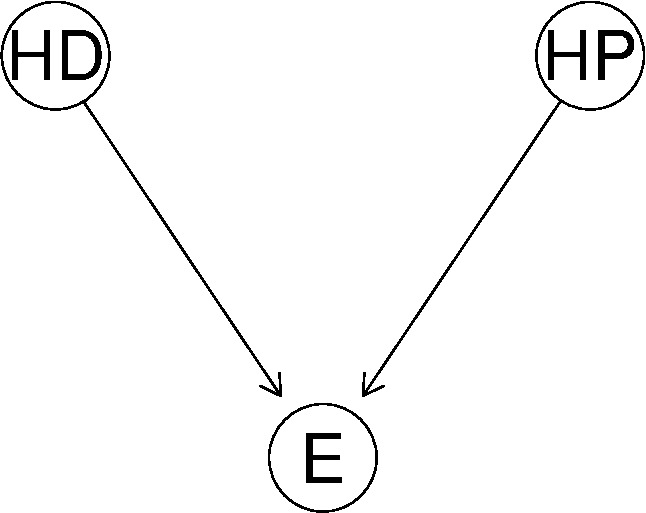
\includegraphics[width=1\linewidth]{lr-chapter4_files/figure-latex/STMdag-1} \end{center}
  \end{subfigure}} \hfill
\begin{subfigure}[!ht]{0.3\textwidth}

\begin{tabular}{lr}
\toprule
HD & Pr\\
\midrule
1 & 0.4\\
0 & 0.6\\
\bottomrule
\end{tabular}


\begin{tabular}{lr}
\toprule
HP & Pr\\
\midrule
1 & 0.02\\
0 & 0.98\\
\bottomrule
\end{tabular}


\begin{tabular}{lllr}
\toprule
\multicolumn{1}{c}{} & \multicolumn{1}{c}{HD} & \multicolumn{1}{c}{HP} & \multicolumn{1}{c}{} \\
E &  &  & Pr\\
\midrule
1 & 1 & 1 & 0.80\\
0 & 1 & 1 & 0.20\\
1 & 0 & 1 & 0.70\\
0 & 0 & 1 & 0.30\\
1 & 1 & 0 & 0.60\\
0 & 1 & 0 & 0.40\\
1 & 0 & 0 & 0.05\\
0 & 0 & 0 & 0.95\\
\bottomrule
\end{tabular}
\end{subfigure}
\caption{Bayesian network and \textsf{CPT}s for a small town murder scenario.}
\label{fig:Cpt}
\end{figure}

Now, \(\pr{E\vert H_d}\) = 0.604, \(\pr{E \vert \n H_d}\) = 0.063, so
\(\mathsf{LR(E, H_d, \n H_d)}\approx\) 9.587, and \(\pr{E\vert H_p}\) =
0.74, \(\pr{E \vert \n H_p}\) = 0.27, and so
\(\mathsf{LR(E, H_p, \n H_p)} \approx\) 3. Crucially, this example is
based on a pair of hypotheses that are neither mutually exclusive nor
exhaustive. As it might in such a case happen, both likelihood ratios
are above one, and so the evidence is not neutral, despite the apparent
intuitions relied on in the counterexample. Moreover, while the evidence
supports each of the hypotheses, the difference in likelihood ratios
indicates that this is so to different extents.\footnote{ de Zoete,
  Fenton, Noguchi, \& Lagnado (2019) offer a slightly different solution
  to the problem. They construct a Bayesian network with three
  hypotheses, also exhaustive and exclusive: in town to visit mother, in
  town to murder, out of town. The gist of the resolution holds, though.}

\mar{R: added this passage in light of Sophie's comments.}

Now, perhaps, one could insist that one at least can think of a case in
which the conditional probabilities: \(\pr{E\vert H_d}\) and
\(\pr{E \vert H_p}\) on one hand, and \(\pr{E\vert \n H_d}\) and
\(\pr{E \vert \n H_p}\), are exactly the same, in which case the
likelihood ratio calculations would fail to shift the probability
balance between the hypothesis. First, such cases would be quite likely
very artificial and unlikely to occur in reality. Second, even in such
cases, we need to recall that Rule 401 talks about the existence of any
fact that is of consequence to the determination of the action, and so
it is enough that there is \emph{some} relevant hypothesis whose
determination becomes easier when the evidence is considered. In the
artificial variant of the small town murder scenario, even if \(H_d\)
and \(H_p\) have the same \text{LR}, there is another pair of relevant
hypotheses that does not: \emph{the suspect was in town} and its
negation.

Analogous considerations should also generalize to other paradoxes of
relevance. For instance, in the twins problem, the LR might be 1 if the
hypotheses are: `the suspect committed the crime,' and `the suspect's
twin brother committed the crime,' but is not 1 if we consider the
fairly natural hypothesis that the defendant is innocent.

Similarly, in the food tray example, Bayesian network analysis shows
that the value of the evidence `prisoner withholds tray' for the
question who started the fight depends on a range of uncertain events
and other pieces of evidence (such as whether indeed a parcel he was
supposed to obtain was withheld; whether the prisoner inquired about
this; whether and how this inquiry was answered). Considered in this
context, the piece of evidence will not have a likelihood ratio of one
with respect to at least some choice of sensible hypotheses.

The general problem with the paradoxes of relevance is that in complex
situations there is no single likelihood ratio that corresponds to a
single piece of evidence. The problematic scenarios focus on a single
likelihood ratio based on non-exclusive or non-exhaustive hypotheses.
However, evidence can be relevant so long as it has a probabilistic
impact on a sub-hypothesis involved in the case, even without having a
recognizable probabilistic impact on the prosecutor's or defense's
ultimate hypotheses. When this happens, it is relevant, in agreement
with Rule 401 of the Federal Rules of Evidence. Bayesian networks help
to see how pieces of evidence can increase or decrease the probability
of different sub-hypotheses (de Zoete, Fenton, Noguchi, \& Lagnado,
2019). Thus, while likelihood ratios are useful, they need to be
properly presented in the context.

\section{Conclusions}

We have introduced likelihood ratio as a measure of evidential strength,
and argued that it is more fit for this purpose in legal contexts than
the Bayes Factor (and, in an appendix, than other probabilistic
confirmation measure).

Then, we moved to the utility of this notion in theorizing about
important factors at play in legal evidence evaluation: false positive
probability of DNA evidence, which should be taken more seriously, and
in the combining of identifying eyewitness evidence with scientific
evidence (and, in appendices on the value of cold-hit DNA matches). Such
considerations, while perhaps fail to provide us with precise
quantitative estimations, tell us what we do not, but should know: false
positive probabilities, and more relevant details of the circumstances
of an eyewitness identification. Had such information been available, at
least rough quantitative estimates of the weight of joint evidence seem
in principle viable, and they seem to be better than mere intuitive
judgment of untrained jury members (also, proper considerations of
cold-hit matches results in a \emph{prima facie} counter-intuitive
result: such matches have higher evidential weight than matches not
obtained through a database search, and doubts about their actionability
have sources elsewhere than in the mere fact that the matches were
obtained through a database search).

\mar{R: revised this in light of Sophie's comments.}

While, conceptually, likelihood ratio seems to be the right tool for the
job of being a local measure of evidential strength, there are some
risks to using likelihood ratios in legal evidence evaluation.
Likelihood ratios are sensitive of this measure to hypothesis choice. In
real-life complex cases multiple hypothesis are available, and proper
evidence evaluation needs to go beyond a single likelihood ratio
statement. The context of an evidence evaluation and such choices should
be made clear and transparent, and proper incorporation of the
likelihood ratios in the judging of a whole case requires a more
elaborate framework and representation of such complexities. A useful
tool fit for this task, we will argue, is Bayesian Network
representation.

\appendix

\addcontentsline{toc}{section}{Appendices}

\section{The cold-hit confusion \label{sec:coldHitConfusion}}

We have been quite negative in the last two sections. What we are after,
though, is a balanced perspective. We are not saying that likelihood
ratios should be disposed of: rather that they should be reported for
individual pieces of evidence and used to evaluate the impact of
combined evidence, but only when proper attention is paid to the
structure of the problem. To re-emphasize the utility of likelihood
ratios when care is paid to both the hypothesis formulation, and to what
the evidence in fact is, we illustrate it by showing how it can be used
to resolve a lengthy debate in legal evidence studies: the value of a
cold-hit DNA match. First, we spend some time explaining the problem in
Appendix \ref{sec:coldHitConfusion}, and then show how LR can be
deployed to resolve it in Appendix \ref{sec:cold-hit}.

First, we explain what a cold hit is and give an example of case based
on a cold hit, the murder of Diana Sylvester. In that case, instead of
random match probability, the defense focused on another measure,
database match probability (DMP). We explain what it is and how it was
recommended to the second National Research Council of DNA Technology in
Forensic Science report. Then we explain how NRC tried to motivate their
recommendation, and why these recommendation are not convincing. This
sets up the stage for the next appendix: if DMP is not the right tool to
evaluate cold-hit evidence, what is?

DNA evidence is one of the most widely used forms of quantitative
evidence currently in use. It may be used to corroborate other evidence
in a case, or as the primary incriminating evidence. For example,
suppose different investigative leads point to an individual, Mark
Smith, as the perpetrator. The investigators also find several traces at
the crime scene left by the perpetrator. Laboratory analyses show that
the genetic profile associated with the traces matches Smith. In this
scenario, the DNA match corroborates the other evidence against Smith.
In contrast, suppose the police has no other investigative lead except
the traces left at the crime scene. Hoping to find the perpetrator, the
police run the genetic profile associated with the traces through a
database of profiles and find a match, a so-called \textbf{cold-hit}.
Cold-hit DNA matches have been the focus of intense discussion in recent
years. Since in cold-hit cases there is little or no other evidence,
cold-hit matches are often the primary item of evidence against the
defendant. Some believe that this circumstance weakens the case. Others
disagree. This debate illustrates how probability theory---in
particular, the likelihood ratio---can help to assess the strength of
evidence at trial. What follows examines some of the main arguments.

For concreteness, consider the California rape and murder case of Diana
Sylvester. In 2008, many years after the crime, John Puckett was
identified as a unique 9-loci match through a database search of 338,000
profiles. He was the only individual in the database who matched the
traces collected from the victim Diana Sylvester in 1972. According to
an expert witness, the particular pattern of alleles present in the
material was (conservatively) expected to occur randomly among Caucasian
men with a frequency of 1 in 1.1 million. This is the
\textbf{random match probability} (\textbf{RMP}). The random match
probability---often interpreted as the probability that someone who is
not the source would coincidentally match,
\(\pr{\textsf{match} \vert \neg \textsf{source}}\)---is a common measure
of the strength of a DNA match. The lower the RMP, the more strongly
incriminating the match. The rationale here is that a low random match
probability suggests that it is unlikely that two people would share the
same DNA profile. In line with what we already discussed, strictly
speaking, a match is a strong evidence that the defendant is the source
only if the probability that the person who left the traces (the
`source') would match is significantly greater than RMP. In practice,
when it comes to DNA evidence, it is often assumed that
\(\pr(\textsf{match} \vert \textsf{source})\) is very high.

Although clearly 1 in 1.1 million should not be confused with the
probability of Puckett's innocence, the small figure indicates it is
very unlikely that a random person unrelated to the crime would match.
The match is therefore strong evidence of Puckett's guilt. Assuming that
the probability of a match if Puckett indeed was the source was
(practically) 1, the likelihood ratio is simply \(1.1 \times 10^6\).

During the pretrial hearing, however, Bicka Barlow, the DNA expert for
the defense, pointed out that this was a cold-hit case. No evidence tied
Puckett to the crime other than the cold-hit match, Puckett's previous
rape convictions, and the fact that he was in the area at the time of
the murder. In order to correctly assess the probative value of the
cold-hit match, Barlow argued, the random match probability should be
multiplied by the size of the database. The result of such a
multiplication is called the \textbf{database match probability}
(\textbf{DMP}). In Puckett's case, the multiplication of
\(\nicefrac{1}{1.1\times 10^6}\) by \(338,000\) resulted in a database
match probability of approximately .3.

\noindent which is a less impressive number than the original RMP (the
likelihood ratio for the DMP is approximately 3.25). According to this
calculation, it was no longer very unlikely that an unrelated person
from the database would match, and so the cold-hit DNA match was no
longer strong evidence of guilt. At least, this was Barlow's argument.

Barlow followed a 1996 report by the National Research Council called
NRC II (National Research Council, 1996), preceded by an earlier report
on DNA evidence called NRC I (National Research Council, 1992). NRC II
recommended precisely what Barlow did: that in cold-hit cases RMP should
be multiplied by the database size, yielding DMP. The underlying idea
was that the larger the size of the dataset, the higher the database
match probability, and the lower the strength of the match. This
correction was meant to guard against the heightened risk of mistaken
matches for the innocent people in the database. To see, however, if
this was sound advice, we need to look under the hood.

The NRC formed the Committee on DNA Technology in Forensic Science,
which issued its first report in 1992. In that report they advised
against using cold hit results as evidence, and insisted that only the
frequencies related to loci not used in the original identification
should be presented at trial, that is, that the evidence used to
identify the suspect should not be used as evidence against the suspect.

This recommendation has been criticized by many because it
underestimates the value of cold-hit matches. The problem was, given a
certain amount of evidence the expert, prior to suspect identification,
had to make a somewhat subjective decision of how to divide the evidence
into two items: one to be used only in the suspect identification, and
one to be used only in the trial itself as evidence against the suspect.
This overly limited the utility of the evidence and introduced an
unnecessary element of
subjectivity.\footnote{It also opened the gate for multiple testing with various evidence division points, and multiple testing leads to its own statistical problems. But let's put this issue aside.}

NRC II withdrew the earlier recommendation. However, the contrast
between low RMP and the frequency of DNA matches in actual database
searchers was indeed stark. For instance, the Arizona Department of
Public Safety searched for matching profiles in a database comprising
65,000 individuals. The search found 122 pairs of people whose DNA
partially matched at 9 out of 13 loci; 20 pairs people who matched at 10
loci; and one pair of people who matches at 12 loci. So it is not that
unlikely to find two people in a database who share the same genetic
profiles (examples of fairly high counts of DNA matches in database
searches was actually used by Barlow in the Diana Sylvester case). In
light of this contrast, NRC II recommended the use of DMP rather than
RMP. NRC II recommended also that in cold-hit cases the likelihood ratio
\(R\) associated with the DNA match should be divided by \(d+1\). Their
first recommendation was about a correction of the random match
probability, and this second recommendation is about the likelihood
ratio.

One argument by NRC employed an analogy involving coin tosses. If you
toss several different coins at once and all show heads on the first
attempt, this seems strong evidence that the coins are biased. If,
however, you repeat this experiment sufficiently many times, it is
almost certain that at some point all coins will land heads. This
outcome should not count as evidence that the coins are biased.
According to NRC II, repeating the coin toss experiment multiple times
is analogous to trying to find a match by searching through a database
of profiles. As the size of the database increases, so does the number
of attempts at finding a match, and it is more likely that someone in
the database who had nothing to do with the crime would match.

Another argument provided by NRC II compared a database trawl to
multiple hypothesis testing, and multiple hypothesis testing should be
avoided if possible in light of classical statistical methods.

Third, NRC II was concerned with the fact that in cold-hit cases the
identification of a particular defendant occurs after testing several
individuals. This concern has to do with the data-dependency of one's
hypothesis: seemingly, the hypothesis `at least one person in a given
database matches the DNA profile in question' changes its content with
the choice of the database.

We will start with the coin analogy. It is in fact unclear how the
analogy with coin tossing translates to cold-hit cases. Searching a
larger database no doubt increases the probability of finding a match at
some point, but is the increase as fast as the Arizona Department of
Public Safety examples and the coin analogy suggest? Quite crucially,
following (Donnelly \& Friedman, 1999) we need to pay attention to what
hypotheses are tested, what probabilistic methods the context
recommends, and what exactly the evidence we obtained is. For instance,
one hypothesis of interest is what we will call a
\emph{general match hypothesis}: \vspace{1mm}

\begin{tabular}{lp{8cm}}
(General match hypothesis) &
At least one of the profiles in the database of size $n$ 
matches the crime sample.
\end{tabular}
\vspace{1mm}

\noindent The general match hypothesis is what NRC II seems to have been
concerned with. If for each data point RMP\(=\gamma\) were held
constant, and if random matches with different data points
\(\mathsf{match_1, match_2, \dots, match_d}\) excluded each other, the
probability of there being at least one random match would be the same
as the probability of their disjunction and could be calculated by the
additivity axiom: \begin{align*}
\pr{\mathsf{at\,\,\, least\,\,\, one\,\,\, match}} & = \pr{\mathsf{match_1} \vee \mathsf{match_2} \vee \cdots \vee \mathsf{match_d}} \\
& = \sum_{i}^d \pr{\mathsf{match_i}} = \gamma \times d
\end{align*} This calculation would result in the outcome recommended by
NRC II, if the value of the evidence were to be a function of the
probability of (General match hypothesis).

The first question is, whether a directly additive calculation should be
applied to database matches. Notice that in applications DMP does not
really behave like probability. Take a simple example. Suppose a given
profile frequency is \(.1\) and you search for this particular profile
in a database of size 10. Does the probability of a match equal
\(.1 \times 10=1\)? The answer is clearly negative. Multiplication by
database size would make sense if we thought of it as addition of
individual match probabilities, provided matches exclude each other and
so are not independent. Here is a coin analogy. Suppose I toss a die,
and my database contains \(n=\) three \emph{different} numbers: \(1, 2\)
and \(3\). Then, for each element of the database, the probability \(p\)
of each particular match is \(\nicefrac{1}{6}\), and the probability of
\emph{at least one} match is
\(\nicefrac{1}{6}+\nicefrac{1}{6}+\nicefrac{1}{6}=\nicefrac{1}{6}\times 3 = n\times p =\nicefrac{1}{2}\).
We could use addition in such a situation because each match excludes
the other matches, a condition that is not satisfied in the database
scenario.

Another reason why DMP is problematic can be seen by taking a limiting
case. Suppose everyone in the world is recorded in the database. In this
case, a unique cold-hit match would be extremely strong evidence of
guilt, since everybody except for one matching individual would be
excluded as a suspect. But if RMP were to be multiplied by the size of
the database, the probative value of the match as measured by DMP should
be extremely low. This is highly counter-intuitive.

Even without a world database, the NRC II proposal remains problematic,
since it sets up a way for the defendant to arbitrarily weaken the
weight of cold-hit DNA matches. It is enough to make more tests against
more profiles in more databases. Even if all the additional profiles are
excluded (intuitively, pointing even more clearly to the defendant as
the perpetrator), the NRC II recommendation would require to devalue the
cold-hit match even further. This, again, is highly counter-intuitive.

Perhaps a somewhat more sensible answer is obtained by assuming the
independence of \(\mathsf{no match}\) for the members of the database
and deploying a solution similar to the one used in the birthday
problem. Here, the idea would be---assuming matches for different data
points are independent and have constant RMP --- to calculate:
\begin{align*}
\pr{\mathsf{match}} & = 1 - \pr{\mathsf{no match}}\\
& = 1 - (1-\gamma)^d
\end{align*} \noindent where \(\gamma\) is RMP, and \(d\) is the
database size. This would be in line with using the binomial
distribution to calculate the probability of no match: \begin{align*}
\mathsf{dbinom}(0,d,\gamma) & = {n \choose 0} \gamma^0 (1-\gamma)^{d-0}\\
& = 1 \times 1 \times (1-\gamma)^d
\end{align*} Now, assuming indeed that \(\gamma\) is constant and that
matches between data points are independent, the dependence of the
probability of at least one match on the database size can be pictured
as in Figure \ref{fig:puckett}.

If we use the RMP and database size used in the Puckett case, the
calculated probability of at least one match is 0.2645501. Not exactly
the DMP postulated by the defendant, but pretty close. The question is,
should this number be the probability used to evaluate the evidential
impact of the cold hit?

One problem is, whether the independence assumption is satisfied in the
database search problem is unclear. After all, if you are informed about
the match frequencies in the database, and they teach you that since two
arbitrary database points quite likely do not match, if the sample
matches one of them, it is less likely to match the other one. And the
independence assumption is not benign. We will illustrate it with a
somewhat distant, but a very striking example, coming from (Barnett,
2020). Suppose you consider whether your effort of casting a vote in the
upcoming election is worth it in a context where there are 500k other
voters. One of the probabilities you might be interested in is the
probability that your vote would make a difference. If we apply the
binomial model to the problem, the probability that a candidate will
receive exactly \(k\) votes if \(n\) people vote is supposed to be
\({n \choose k} p^{k} (1-p)^{(n-k)}\), where votes of the population
members are supposed to be independent and estimated to have the same
probability \(p\) of being for the candidate. For instance, if 500k
people vote and \(p= 0.5\), the probability that the candidate will
receive exactly 250k votes is 0.0011284, which is around
\nicefrac{1}{886} and much higher than \(\nicefrac{1}{n}\). This fairly
high chance made some claim that the chance that your voice is decisive
if the chances are equal is fairly high in such circumstances. However,
note that if \(p=.505\), the probability that the candidate will receive
exactly 250k votes is \ensuremath{1.5651281\times 10^{-14}}, which is
less than one in a trillion. This lead some (Brennan, 2012;
\emph{Democracy and decision}, 1993) to claim that outside of the very
specific circumstances, decision-theoretic arguments for the rationality
of voting are hopeless. Barnett, however, points out that such a
sensitivity to success probability simply makes the binomial model
inappropriate for the voting context, observing that its calculations
also disagree with empirical estimates which are not too far from
\(1/n\) (Gelman, Katz, \& Tuerlinckx, 2002; Gelman, King, \& Boscardin,
1998; Mulligan \& Hunter, 2003). This sensitivity arises, because within
the binomial model the more trials (voters) there are, the more tightly
the results will tend to cluster around the probability of success. To
observe how unrealistic that is, keep \(p=.505\) and ask yourself how
probable it is that the voting result will be between \(50.4\%\) and
\(50.6\%\). Sure, this outcome might be quite likely, but the binomial
certainly overestimates it at 0.8427212. Another unrealistic estimate
obtained by the binomial model is the estimate of the probability of an
upset (that the leading candidate will lose). With \(p=.505\) this is
\(\mathsf{pbinom(249999,500000,.505)}\), which turns out to be extremely
and unrealistically low: \ensuremath{7.5994495\times 10^{-13}}.

\raf{M: Pretty interesting, but in the voting model, it seems that feedback mechanisms betewen voters affect behaviour, but not so in the genetic case. Can you spell out the analogy more clearly?}
\mar{Not sure what you mean, we should talk about this.}

\begin{figure}[h]

\begin{center}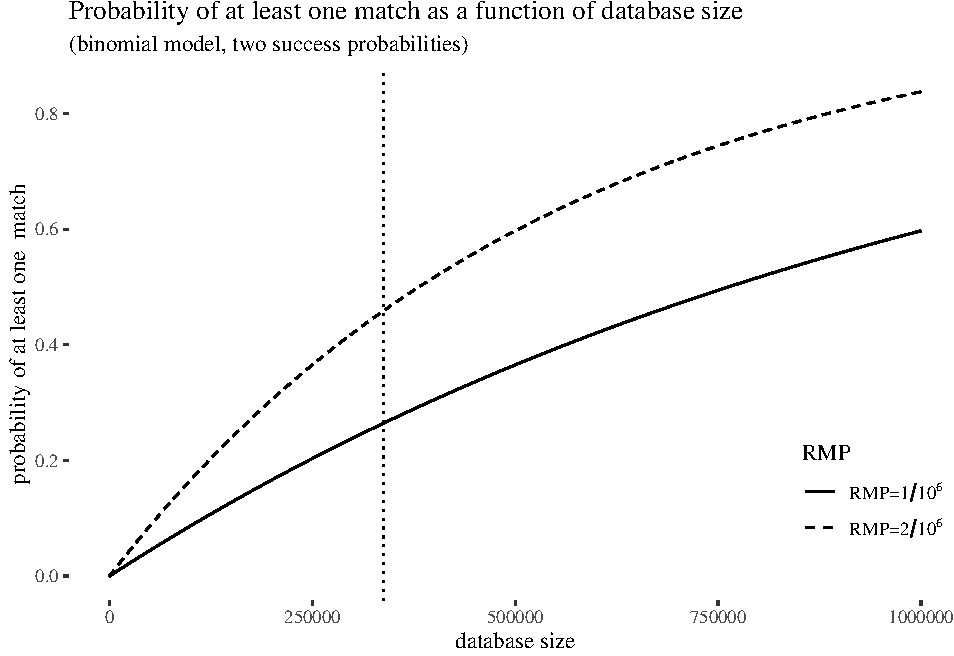
\includegraphics[width=0.8\linewidth]{lr-chapter4_files/figure-latex/fig-puckett-1} \end{center}
\label{fig:puckett}
\caption{Binomial model of the database search problem. The probability of at least one match depending on the database size, assuming independence and constant RMP used in  the Puckett case as compared with the binomial estimate for p=2/1.1e6 (dashed line). The actual database size marked with a vertical line."}
\end{figure}

Coming back to our original problem, the binomial estimate of the
probability of a match is also quite sensitive to RMP, as illustrated in
Figure \ref{fig:puckett}. The bottom line is that if we have reasons to
think the independence assumption is not satisfied, the binomial model
is not appropriate. So, it seems, it is not appropriate for the database
match problem either.

The binomial model, however, is useful, in its simplicity, for
illustrating an important distinction whose conflation underlies one of
the involved arguments. You might have been surprised learning that
while the expert testified that RMP on 9 loci for Puckett was 1 in 1.1
million, the Arizona Department of Public Safety found 122 9-loci
matches among 65,000 individuals. After all, 122/65000 is 0.0018769,
which is much higher than the reported RMP.

Crucially, notice that there is a difference between having a sample and
looking for a match in a database of size \(n\) and taking a database of
size \(n\) and checking all pairs that occur within it for a match. In
the former case, you are making \(n\) comparisons. In the latter case,
the number of comparisons is \({n \choose 2}\), which is much higher. If
\(n=65000\), there are \ensuremath{2.1124675\times 10^{9}} pairs to
compare, so while the binomial estimate of the probability of at least
one match for \(n\) comparisons (the former case) is 0.057379, it is
approximately 1 for \({n \choose 2}\) comparisons. For the impact it has
on the Arizona Department of Public Safety statistics, consider the
binomial estimate of the probability of at least 122 matches among all
pairs as a function of the database size, even for relatively low
database size range (up to 50000), as illustrated in Figure
\ref{fig:Arizona}.

\begin{figure}[h]

\begin{center}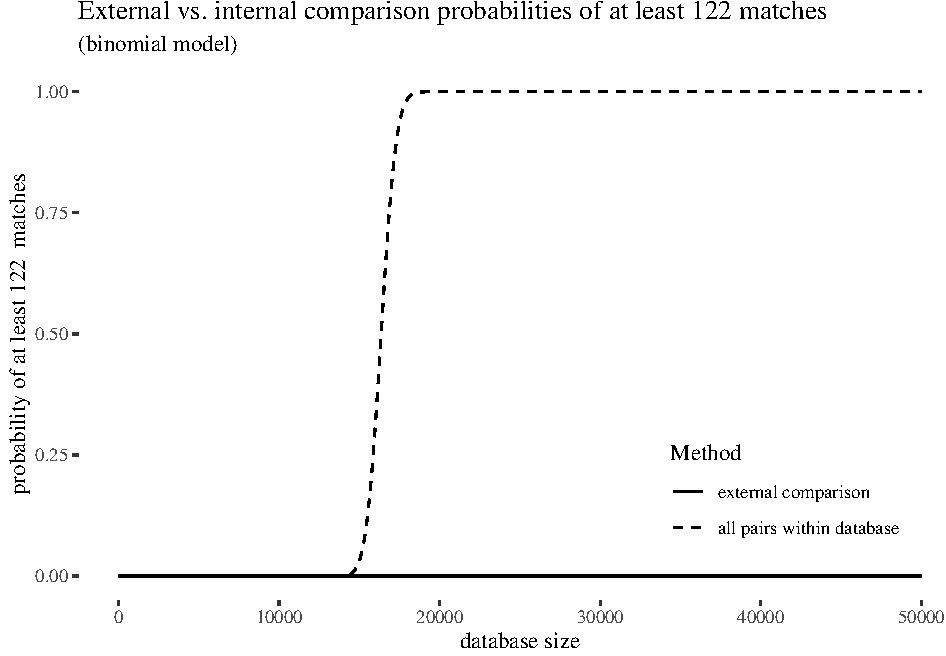
\includegraphics[width=1\linewidth]{lr-chapter4_files/figure-latex/fig-Arizona-1} \end{center}
\caption{Binomial model of the database search problem. The probability of at least 122 matches depending on the database size for n comparisons with an external sample, and for all possible pairs among n datapoints (dashed), assuming RMP=1/1.1e6.}
\label{fig:Arizona}
\end{figure}

From this perspective, it is no surprise there were so many matching
pairs among all the pairs from the database. Unfortunately, this
frequency does not estimate the probability of at least one match in the
set-up we are actually interested in. After all, in a cold-hit scenario
we do have a sample outside of the database and make \(n\) comparisons,
instead of testing all possible pairs from the database for a match.

Before we move on, it is worthwhile to think about how the example at
hand actually constitutes evidence against a certain probabilistic model
that one might initially want to deploy in this context. Note how the
Arizona statistics constitute some empirical evidence against the
adequacy of the binomial model. While the binomial estimate probability
of at least 122 matches with an external sample for \(n=6500\) is pretty
much 0, let us look at the most likely number of matches if we test
\({6500 \choose 2}\) pairs, as estimated by the binomial model. We
illustrate it with an 89\% highest density interval in Figure
\ref{fig:ArizonaDensity}. So, if the expert's estimate and the binomial
model are both adequate, we indeed should be surprised by the presence
of 122 matches. But this is because this number is surprisingly low:
instead we should expect a much higher number, around 2000 of them! OF
course, it is unlikely that in fact all possible pairs have been
compared, and it is hard to evaluate this evidence against the binomial
model unless we know the exact number of comparisons made.

\begin{figure}[h]

\begin{center}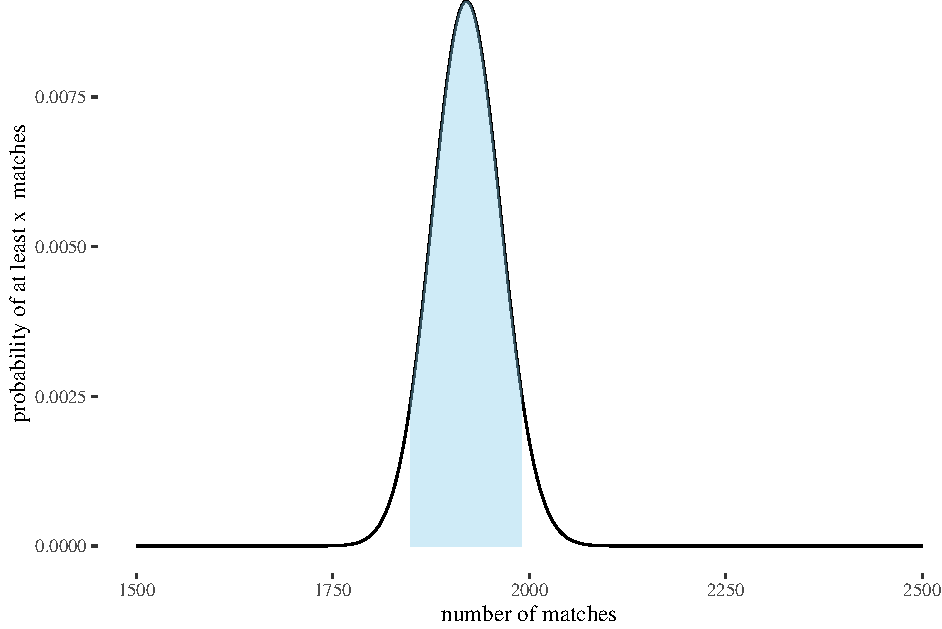
\includegraphics[width=1\linewidth]{lr-chapter4_files/figure-latex/fig:ArizonaDensity-1} \end{center}
\caption{Binomial probability density of  n matches in pairwise comparison within a database of size 65000, assuming $p=1/1.1e6$, with 89\% highest density interval $=(1849,1990)$ shaded in blue.}
\label{fig:ArizonaDensity}
\end{figure}

Now that we used the imperfect binomial model to clear up at least one
confusion, let us put it aside, and focus on an even deeper problem with
using the probability of (General match hypothesis) instead of RMP in
evidence evaluation. Probabilistic epistemology recommends that once we
obtain new evidence, our new degrees of belief should be the
probabilities obtained by conditionalizing on this evidence. Crucially,
we should update on the total evidence we obtained rather than only on a
part of it. Here the question is, does (General match hypothesis)
exhaust what we have learned from our database match?

To get us started thinking about this question, consider a coin analogy
which Donnelly \& Friedman (1999, p. 950) found more adequate than the
one proposed by the NRC. Imagine a biased coin whose physical appearance
is indistinguishable from the fair coins in a piggy bank. The biased
coin is the perpetrator and the piggy bank is the database containing
innocent people. After the biased coin is thrown into the bank with the
other coins, someone picks out a handful of coins at random and flips
each of them twenty times. Each coin lands heads approximately ten
times---except for one coin, which lands heads on all twenty flips. The
fact that other coins seem unbiased makes the claim that this one is
biased\\
better supported.

Coming back to DNA matches, think about the following scenario: first,
you identified the suspect by some means other than a database trawl.
Then, it turned out his DNA profile matches the crime scene stain. Fine,
here it seems uncontroversial that this constitutes strong further
incriminating evidence. Now, imagine a further database search in a
database not containing this suspect finds no matches. Would you think
that this information supports the guilt hypothesis? If your answer is
yes, then you do have the intuition that the lack of matches with other
people (whose profiles, in this particular case, happen to be in a
database) strengthens the evidence.

The key lesson here (and in the complete-world database scenario we
already discussed) is that we not only learned that there was a match in
the database of size \(n\), but also that in \(n-1\) cases there was no
match, and this information also has evidential value. In line with
this, contrary to NRC II, Donnelly \& Friedman (1999) argues that if
potential suspects in the database are excluded as sources, this should
increase, not decrease, the probability that the defendant who matches
the crime traces is the source. A cold-hit match, then, is stronger and
not weaker evidence of guilty than ordinary DNA matches.

Before moving on to a better model that captures how this could be, let
us look at another argument put forward by NRC, an analogy to multiple
hypothesis testing. NRC claimed that there is an analogy between
searching for a match in a database and multiple hypothesis testing,
which is a dubious research practice. In classical hypothesis testing,
if the probability of type I error in a single test of a hypothesis is
5\%, the probability of at least one type I error will increase by
testing the same hypothesis multiple times. In analogy---the argument
goes--- we need to correct for the increased risk of type I error, and
just as the Bonferroni correction requires that the \(p\)-value
threshold be divided by the number of tests, NRC II requires that the
estimated probability of a random match should be multiplied by the
number of comparisons.

This analogy with multiple testing, however, is misplaced. As David J.
Balding (2002) points out, multiple testing consists in testing the
\textit{same} hypothesis multiple times against new evidence. In
cold-hit cases, no such multiple testing is involved. Rather, multiple
hypotheses---each concerning a different individual in the
database---are tested only once and then excluded if the test is
negative. From this perspective, for each \(1 < i <n\), the following
hypothesis is tested: \vspace{1mm}

\begin{tabular}{lp{8cm}}
(Particular match hypothesis) &
Profile $i$ in the database matches the crime sample.
\end{tabular}
\vspace{1mm}

\noindent and the hypothesis that the defendant is the source was one of
the many hypotheses subject to testing. The cold-hit match supports that
hypothesis and rules out multiple other hypotheses.

\section{ Likelihood ratio and cold-hit DNA matches \label{sec:cold-hit}}

To find a better path towards the resolution of the database search
problem, let us look at another recommendation of NRC II, that in
cold-hit cases the likelihood ratio \(R\) associated with the DNA match
should be divided by \(n+1\), where \(n\) is the database size. This
approach has been defended defended by (Stockmarr, 1999), who points out
that since the suspect is identified after the databases search, the
hypothesis is formulated \textit{ad hoc}. Without the correction, then,
the likelihood ratio would be data-dependent. For instance, he insists
that hypotheses such as \emph{JS was one of the crime scene donors} are
evidence-dependent in the case of database search, ``since we had no way
of knowing prior to the search that Smith would be the person that
matched'' (p.~672). Instead, Stockmarr claims, we should evaluate LR
using hypotheses that can be formulated prior to the search, such as
\emph{the true perpetrator is among the suspects identified from the database}.
And indeed, the likelihood of this hypothesis is as NRC II suggests,
\(\nicefrac{k}{np}\), where \(k\) is the number of matching profiles,
\(n\) the database size, and \(p\) the random match probability (see
Stockmarr, 1999 for a derivation).

Dawid, in a discussion with Stockmarr (Dawid \& Stockmarr, 2001) points
out that Stockmarr's hypotheses, while not depending on the result of
the search, depend on the data themselves (because they change with the
database size). More importantly, he also indicates that Stockmarr's
hypotheses are composite and the assessment of LR therefore requires
additional assumptions about the priors. Once these are used with
Stockmarr's own LR, the posterior is the same as the one obtained using
the methods proposed by the critics of NCR II. This is a particular case
of a general phenomenon that we will discuss later on: different
hypotheses might result in different LR, but be equivalent conditional
on the evidence, and so result in the same posterior probabilities. This
general phenomenon indicates how LR on its own might be insufficiently
informative.\footnote{See however, Stockmarr's own reply
  (\emph{ibidem}).}

Putting Stockmarr's defense and its problems aside, the NRC II
recommendation is questionable on more principled grounds. Suppose \(R\)
is not too high, say because the identified profile is common since the
crime scene DNA is degraded and only a few markers could be used. Then,
\(n+1\) can be greater than \(R\), so \(R/(n+1)<1\). The match would
then be exculpatory, a very counter-intuitive result. Moreover, if the
defendant on trial is the source, the probability that he would match is
practically 1. If he is not, the probability that he would still match
equals the random match probability. Neither of these probabilities
change because other suspects have been tested in the database search.
In fact, if potential suspects are excluded as potential sources, this
should increase, not decrease, the probability that the defendant who
matches the crime traces is the source.

A more principled way to assess cold-hit matches based on the likelihood
ratio, exists. The proposal draws from the literature on the so-called
\textbf{island problem}, studied by (Dawid, 1994; Dawid \& Mortera,
1996; Eggleston, 1978). Let the prosecutor's hypothesis \(H_p\) be `The
suspect is the source of the crime traces' and the defense's hypothesis
\(H_d\) be `The suspect is not the source of the crime traces.' Let
\(E\) be the DNA match between the crime stain and the suspect (included
in the database) and \(D\) the information that none of the \(n-1\)
profiles in the database matches the crime stain. The likelihood ratio
associated with \(E\) and \(D\) should be (David J. Balding \& Donnelly,
1996; Taroni, Biedermann, Bozza, Garbolino, \& Aitken, 2014):
\begin{align*}
V & = \frac{\pr{E,D\vert H_p}}{\pr{E,D\vert H_d}}.
\end{align*} Since \(\pr{A\wedge B}=\pr{A\vert B}\pr{B}\), for any
statement \(A\) and \(B\), this ratio can be rewritten as:
\begin{align}\label{eq:lrdna1}
V & = \frac{\pr{E\vert H_p,D}}{\pr{E\vert H_d,D}} \times \frac{\pr{D\vert H_p}}{\pr{D\vert H_d}}.
\end{align} \noindent The first ratio in \eqref{eq:lrdna1} is roughly
\(\nicefrac{1}{\gamma}\), where \(\gamma\) is the random match
probability. The second ratio--- call it the
\textbf{database search ratio}---requires some more work. Consider first
the denominator \(\pr{D \vert H_d}\). If the suspect is not the source
(\(H_d\)), someone else is, either someone who is in the database or
someone not in the database. Let \(S\) stand for
\textsf{The  source is someone in the database.} By the law of total
probability, \begin{align}\label{eq:dnaLOTP}
\pr{D\vert H_d} & = \pr{D\vert S, H_d} \pr{S\vert H_d} + \pr{D\vert \neg S, H_d} \pr{\neg S \vert H_d}. 
\end{align} If the source is someone in the database (\(S\)) and the
suspect is not the source (\(H_d\)), it is very unlikely that no one in
the database would match (\(D\)), so \(\pr{D\vert S, H_d}\approx 0\).
The equality in \eqref{eq:dnaLOTP} therefore simplifies to:
\vspace{-4mm} \begin{align*}
\pr{D\vert H_d} & =  \pr{D\vert \neg S, H_d} \pr{\neg S \vert H_d}, 
\end{align*} \noindent The database search ratio would therefore be:
\begin{align*}
\frac{\pr{D\vert H_p}}{\pr{D\vert H_d}} & = \frac{\pr{D\vert H_p}}{\pr{D\vert \neg S, H_d} \pr{\neg S \vert H_d}}.
\end{align*} \noindent Note that
\(\pr{D\vert H_p}=\pr{D\vert \neg S, H_d}\) because whether the suspect
is the source (\(H_p\)) or not (\(H_d\)) does not affect whether there
is a match in a database that does not contain the source (\(\neg S\)).
Let the probability that no person in the database other than the
suspect would match (\(D\)), assuming the suspect was in fact the
source, be \(\psi_{n-1}\). Notice that \(\pr{D\vert \neg S, H_d}\) is
the probability that no one other than the suspect matches in the
database that does not contain the real source, if the suspect is not
the source. So this conditional probability can also be estimated as
\(\psi_{n-1}\).\footnote{If the prior probability that the perpetrator is in the database was high, the calculations would need to be different. But normally, this prior is not too high.}
Let \(\pr{S | H_d}=\varphi\). The database search ratio then would
reduce to \vspace{-2mm} \begin{align*}
\frac{\pr{D\vert H_p}}{\pr{D\vert H_d}} & = \frac{1}{1-\varphi}.
\end{align*} \noindent As the database gets larger, \(\varphi\)
increases and the database search ratio also increases. This ratio
equals one only if no one in the database could be the source, that is,
\(\varphi=0\).\\
Since the likelihood ratio \(V\) of the cold-hit match results by
multiplying the likelihood ratio of the DNA match and the database
search ratio, \(V\) will always be greater than the mere likelihood
ratio of the match (except for the unrealistic case in which
\(\varphi=0\)) . Thus, a cold-hit DNA match should count as stronger
evidence than a DNA match of a previously identified suspect.

Dawid \& Mortera (1996) study different database search strategies and
consider the possibility that information about the match is itself
uncertain, but the general point remains. Under reasonable assumptions,
ignoring the database search would give a conservative assessment of the
evidential strength of the cold-hit match. Donnelly \& Friedman (1999),
with slightly different assumptions, derived the formula
\(R \times [1+md/N]\), where \(R = 1/\gamma\), \(d\) is the database
size, \(N\) the number of people in population not in database, and
\(m\) is an optional multiplier reflecting how much more likely persons
in the database are though to be the source when compared to the rest of
the population. The expression cannot be less than \(\gamma\). If no
other profile has been tested, \(d=0\) and LR is simply the regular DNA
match LR. If \(N\) is zero, that is, everyone in population is in the
database, the result is infinitely large.

This proposal is able to accommodate different apparently competing
intuitions. First, consider the intuition that as the size of the
database grows, it is more likely that someone in the database would
match. This intuition is captured by the fact that \(\varphi\) increases
proportionally to the size of the database even though this increase
does not imply that the evidential value of the cold-hit match should
decrease. Second, there is intuitive resistance to basing a conviction
on a cold-hit match, although this resistance is less strong in case of
an ordinary match (more on this later in Section
\ref{sec:naked}).\todo{Fix crossref later} This preference for
convictions based on an ordinary DNA match seems in tension with the
claim that a cold-hit match is stronger evidence of guilt than an
ordinary match. There is a way to make sense of this, though. The key is
to keep in mind that the evidential strength---measured by the
likelihood ratio---should not be confused with the posterior probability
of guilt given the evidence. Even if a cold-hit match is stronger
evidence of guilty, this fact does not imply that the posterior
probability of the defendant's guilt should be higher.\\
If the cold-hit match is the only evidence of guilt, the posterior
probability of guilt may well be lower compared to cases in which other
evidence, such as investigative leads, supplements the DNA match. This
lower posterior probability would justify the intuitive resistance
towards convictions in\\
cold-hit cases, despite the fact that a cold-hit match alone is stronger
evidence than a DNA match obtained otherwise and taken on its own.
Moreover, it is possible that the intuitive assessment of cold-hit
evidence takes to some extent the impact of false positive probability
into account.

\raf{M: We need a proper conclusion here. Now it feels as thought LR are a good thing, at leats for cold-hits. But is this just an exception? Do LR have a very narrow applicability, say only for DNA evidence? So where do we stand exactly? And what about BF and Bayesian networks and priors? Need general morals here.}

\mar{I think I now reiterated our point too many times throughought the chapter, we'll discuss this.}

\section{ Confirmation measures \label{sec:confirmation}}

At this point a philosophically minded reader might recall that there is
an important notion in the vicinity---that of confirmation---and that
there is a vast philosophical literature on probabilistic explication of
that notion. Natural questions arise: how is the notion of confirmation
related to the notion of evidence strength, and why almost none of the
probabilistic explications of confirmation have not been deployed in
legal probabilism?

The key question behind the enterprise we are going to take a look at
is: when does a piece of evidence confirm a theory, and how are these
requirements to be explicated probabilistically to agree with both
successful scientific practice and sensible philosophical principles?
The hope is that having answered these questions would facilitate both
rational reconstructions of various developments in the history of
science, and a critical evaluation of various ongoing scientific
investigations.

The underlying probabilistic idea is that the level of confirmation of a
theory (\(T\)) by a piece of evidence (\(E\)) is a function of an
agent's degrees of belief. The first stab might be, let's simply
identify the confirmation level with \(\pr{T \vert E}\). This, however,
is way too quick. Multiple factors come into the assessment of this
conditional probability, and two agents can agree on the extent to which
\(E\) confirms \(T\) without agreeing on the posterior probability of
\(T\) (identified with \(\pr{T \vert E}\)), because the agents might
disagree about the prior probability of \(T\) and this might have an
impact on the posterior.

Still, some requirements on confirmation measures can be formulated in
terms of probabilities. One usual assumption (Sprenger \& Hartmann,
2019) is that the level of confirmation is to be a continuous function
of \(\pr{T}\) and \(\pr{E\vert T}\) which is non-decreasing in the first
argument and non-increasing in the second argument. That is, increasing
the prior, should not lower the confirmation level, and increasing the
likelihood should not increase the confirmation level. Let's call this
condition the \emph{prior-posterior dependence}.\footnote{Some
  formulations (Crupi, 2015) are a bit more general and include
  background knowledge \(K\). In that setting, the corresponding
  requirement is called \emph{Formality} and takes the confirmation to
  be a function of \(\pr{H \et E \vert K}, \pr{H\vert K}\) and
  \(\pr{E\vert K}\). For the sake of simplicity, we will suppress the
  reference to \(K\), unless required by the context.}

One consequence of the prior-posterior-dependence---called
\emph{Final Probability Incrementality} is that confirmation of \(T\) by
\(E\), \(c(T,E)\) should track the posterior order-wise, that is
\(c(T,E)>c(T,E')\) just in case \(\pr{T\vert E} > \pr{T\vert E'}\).

Another requirement is that there should be a neutral point \(n\) such
that \(E\) confirms (disconfirms) \(T\) just in case \(c(T,E)>n\)
(\(c(T,E)<n\)) and is neutral exactly at \(n\). This is called the
\emph{qualitative-quantitative bridge}.

Yet another requirement is \emph{local equivalence}. Theories that are
logically equivalent given the evidence should receive equal
confirmation from this evidence. Interestingly, all confirmation
measures which satisfy prior-posterior dependence,
qualitative-quantitative bridge, and local equivalence are strictly
increasing functions of \(\pr{H \vert E}\). Such measures are said to
explicate confirmation as \emph{firmness of belief}. Moreover, all
functions satisfying these three conditions are ordinally
equivalent.\footnote{Measure $c$ is ordinally equivalent to measure $c'$ just in case always $c(E , T) \gtreqqless c(E', T')$ iff $c'(E , T) \gtreqqless c'(E' , T')$.}

However, another notion of confirmation seems often at play. For
instance, even if the posterior \(T\) is low, one might still think that
a given experiment speaks strongly in favor of \(T\). And relatedly,
\(E\) can lower the posterior of \(T\) while still leading the posterior
to be sufficiently high for the firmness confirmation measure to be
above the neutrality threshold. Another feature of confirmation as
firmness is that if, in this sense, \(T\) confirms \(H\), then for any
\(H'\) that is excluded by \(H\), \(T\) disconfirms \(H'\). But now
think of the small town murder scenario we already discussed: the fact
that the suspect was seen in town seems to support both the prosecution
hypothesis that he committed the murder, and the defense hypothesis,
that he was in town to visit his mother. Confirmation as firmness cannot
capture such intuitions, as relevance cannot be captured as a function
of the posterior alone.

For such reasons, following the second edition of (Carnap, 1962), it is
customary to distinguish another notion in the vicinity: confirmation as
increase in firmness of belief. If we replace local equivalence with
tautological equivalence \(c(T, \top) = c(T', \top)\), where \(\top\) is
a logical tautology---the idea being that hypotheses are equally
supported by empty evidence---we end up with another class of
confirmation measures, those meant to capture
\emph{probabilistic relevance}. On this approach, \(E\) confirms
(disconfirms) \(T\) just in case \(\pr{H \vert E} > \pr{H}\)
(\(\pr{H \vert E} < \pr{H}\)).

Here is a list of key confirmation measures available on the market
(Sprenger \& Hartmann, 2019), normalized so that they all have neutral
points at 0:

\begin{align}
\tag{Difference}  D(T,E) & = \pr{T\vert E} - \pr{T}\\
\tag{Log-ratio}  Lr(T,E) &  = log\left(\frac{\pr{T\vert E}}{\pr{T}} \right) \\
\tag{Log-likelihood}   LL(T,E) & = log\left(\frac{\pr{E \vert T}}{\pr{E \vert \n T}} \right)\\
\tag{Kemeny-Oppenheim}  K(T,E) & = \frac{\pr{E\vert T} - \pr{E \vert \n T}}{\pr{E \vert T} + \pr{E \vert \n T}} \\
\tag{Generalized entailment}  Z(T,E) & = \begin{cases}
\frac{\pr{T\vert E} - \pr{T}}{1-\pr{T}} & \mbox{ if } \pr{T \vert E} \geq \pr{T}\\
\frac{\pr{T\vert E} - \pr{T}}{\pr{T}} & \mbox{ if } \pr{T \vert E} < \pr{T}
\end{cases} \\
\tag{Christensen-Joyce} S(T,E) & = \pr{T \vert E} - \pr{T \vert \n E} \\
\tag{Carnap}  C(T,E) & = \pr{E}(\pr{T\vert E} - \pr{T})\\
\tag{Rips} R(T\vert E) & = 1 - \frac{\pr{\n T\vert E}}{\pr{-T}}
\end{align}

(Log-likelihood), our good old likelihood ratio, and (Kemeny--Oppenheim)
are ordinally equivalent (and no other pair on the list is). The former
makes calculations of joint support additive, and the former has the
nice feature of ranging from \(-1\) to \(1\) and having 0 as a neutral
point, so if one accepts the use of likelihood ratio, these two also can
be used on some occassions when these additional features are justified.
Further grouping and assessment of the confirmation measures for a given
purpose is facilitated by the following facts:

\begin{itemize}
\item
  One might require that \(E\) always confirms the disjunction of
  excluding hypotheses more than one of them just in case it also
  confirms the other one (\emph{disjunction of alternative hypotheses}).
  This can happen only if the confirmation measure is a strictly
  increasing function of the difference measure. Whether this is an
  intuitive requirement in our context is unclear.
\item
  One might require that confirmation should track
  likelihood---\(c(T,E) > c(T,E')\) (\emph{Law of likelihood})---just in
  case \(\pr{E\vert T} > \pr{E'\vert T}\). This can happen only if the
  measure is a strictly increasing function of the Bayes factor. At
  least in legal applications, the law of likelihood is suspicious, as
  our example with rocking child abuse victims discussed on page
  \ref{text:rock} indicates.
\item
  You might wish that confirmation be \emph{contrapositive}
  (\(c(T,E) = c(\n E, \n T))\) and \emph{commutative}
  (\(c(H,E) = c(E,H)\)). The only measures that satisfy both are
  relative distance measures, that is, they are strictly increasing
  functions of the generalized entailment measure.
\item
  One might require that if \(E\) and \(E'\) are conditionally
  independent given \(T\) and \(\neg T\), then \(c(T,E)\) should be
  identical with \(c(T,E\vert E')\) (the confirmation obtained when
  \(E'\) is added to the background knowledge). This condition is called
  \emph{modularity}. This condition holds only if a confirmation measure
  is a strictly increasing function of the likelihood ratio.
\end{itemize}

Moreover, if you require strict additivity:
\(c(H, E\et E') = c(H, E) + c(H, E'\vert E)\), the only measure that
satisfies the disjunction of alternative hypotheses is the difference
measure, the only measure that satisfies the law of likelihood is the
log-ratio measure, and the only one that satisfies modularity is the
log-likelihood measure.

Some unity can be brought into the picture (Crupi, Tentori, \& Gonzalez,
2007) by normalizing by what happens with a measure where logical
consequence or exclusion is involved. For instance, if \(E \vert T\),
\(D(E,T)=\pr{\n T}\) and if \(E\vert \n T\), \(D(E,T) = - \pr{T}\). So
the normalized version has the form: \begin{align*}
D_n(E,T)  & = \left\{ \begin{array}{lr}
\nicefrac{D(E,T)}{\pr{\n T}} & \mbox{ if } \pr{T\vert E} \geq \pr{T}\\
\nicefrac{D(E,T)}{\pr{H}} &\mbox { otherwise.}\\
\end{array} \right.
\end{align*}

Interestingly, analogous normalization of measures other than
(Generalized entailment) leads to the same single new Bayesian measure
of confirmation: (Generalized entailment). Another reason one might have
to like this measure is as follows. Take any \(k > 0\) and say
\(v(E,T) =k\) iff \(E\models T\), \(v(E,T) = -k\) iff \(E \models \n T\)
and \(v(E,T)=0\) otherwise. The \emph{logical closure requirement} is
that if \(v(E,T) > v(E', T')\), then \(c(E, T) > c(E' , T' )\). It turns
out that all measures ordinally equivalent to the listed measures other
than (Log-likelihood), likelihood ratio, (Generalized entailment) fail
to satisfy this condition and Z, likelihood ratio, (Kemeny-Oppenheim)
and (Kemeny-Oppenheim) succeed at satisfying it.

Now, what reasons do we have to not use some of the measures we
introduced? First, some insights are obtained by considering the
abstract requirements. Crucially, (1) final probability incrementality
with prior-posterior dependence exclude (Carnap) and
(Christensen-Joyce), (2) (Carnap) and (Log-ratio) have the unintuitive
consequence that \(C(T,E)= C(E,T)\) (call this \emph{symmetry}), (3)
(Difference), (Generalized entailment), (Log-ratio), (Carnap) and (Rips)
depend on the prior of \(T\), and (4) logical closure requirement
excludes many of the measures.

Moreover, there is an issue with \(Z\) (Branded Fitelson, 2021). Say
\(E\) and \(E'\) are confirmationally independent regarding \(H\) just
in case both \(c(T, E \vert E' ) = c(T, E )\) and
\(c(T, E' \vert E ) = c(T, E')\) Say \(E\) and \(E'\) are conflicting
evidence regarding \(T\) iff \(\pr{T\vert E}> \pr{T}\) while
\(\pr{T\vert E'} < \pr{T}\). Branded Fitelson (2021) has proven that any
measure ordinally equivalent with \(Z\), however, excludes the fairly
intuitive possibility of the existence of confirmationally independent
and yet conflicting evidence (he also gives a clear example of such a
case).

Last but not least, for legal applications it seems that dependence on
the prior probability is undesirable. We propose that at least two
conceptual takes on confirmation is available. On one hand, say a
scientific community pretty much agrees on the status of a given theory
prior to an experiment. Then, after the experiment, it is a legitimate
question what impact the experiment has on the status of that theory,
and perhaps it makes sense that the prior status of that theory plays a
role. On the other hand, in legal context, we would like (1) the
expert's assessment not to depend on the expert's prior convictions
about the hypothesis, and (2) the expert's statement to mean the same
for various agents involved in the fact-finding process, even if they
assign different priors to the hypothesis. For this reason, we propose
that dependence on priors in legal evidence evaluation is an undesirable
feature of a confirmation measure.

Thus, the general picture obtained, pictured in Table
\ref{tab:confirmation}, seems to suggest that the likelihood ratio is a
decent choice for our applications. This, of course, also applies to
(Log likelihood) and (Kemeny-Oppenheim), which are ordinally equivalent
to likelihood ratio, but the reasons to not use them in a legal context
are that (Kemeny-Oppenheim) is conceptually more complex than likelihood
ratio, and that thinking in terms of logarithms is not very natural for
human agents.

\begin{table}
\centering\begingroup\fontsize{9}{11}\selectfont

\begin{tabular}{lp{10cm}}
\toprule
Measure & Reason not to use\\
\midrule
\cellcolor{gray!6}{(Difference)} & \cellcolor{gray!6}{dependence on priors, logical closure failure}\\
(Log-ratio) and (Bayes factor) & satisfies law of likelihood, symmetry, dependence on priors, failure to satisfy logical closure\\
\cellcolor{gray!6}{(Generalized entailment)} & \cellcolor{gray!6}{dependence on priors, independent conflicting evidence}\\
(Christensen-Joyce) & excluded by final probability incrementality with prior-posterior dependence\\
\cellcolor{gray!6}{(Carnap)} & \cellcolor{gray!6}{excluded by final probability incrementality with prior-posterior dependence, symmetry, logical closure failure}\\
(Rips) & dependence on priors, failure of logical closure\\
(Christensen-Joyce) & excluded by final probability incrementality with prior-posterior dependence\\
\cellcolor{gray!6}{(Kemeny-Oppenheim)} & \cellcolor{gray!6}{none of the above, but unnecessarily complex}\\
(Log likelihood) & none of the above, but logarithms are hard for humans\\
\cellcolor{gray!6}{(Likelihood ratio)} & \cellcolor{gray!6}{none of the above}\\
\bottomrule
\end{tabular}
\endgroup{}
\caption{Reasons not to use various confirmation measures in legal fact-finding applications.}
\label{tab:confirmation}
\end{table}

\mar{R: so here's my account of the Heckerman's result, take a look}

Finally, here is a somewhat abstract, yet important approach to
confirmation measures due to (Heckerman, 1988), which constitutes a
fairly strong motivation to use likelihood ratio. Suppose you have
background information \(e\), and consider a hypothesis \(H\) when you
obtain a piece of evidence \(E\). A belief update, \(U(H, E, e)\),
together with your prior stance of \(H\), should determine your
posterior belief in \(H\). If we denote conditional belief in \(H\)
given \(E\), without assuming it's probabilistic yet, as \(H\vert E\),
this means that there should be an \(f\) such that: \begin{align*}
H \vert Ee & = f(U(H,E,e), H \vert e)
\end{align*}

\noindent where, on this approach, \(H \vert Ee, U(H,E,e),\) and
\(H \vert e\), are all real numbers, and \(f\) is required to be
continuous in both arguments and monotonically increasing when the other
is held constant. Call this the \textbf{update requirement}. Bayesian
updating is a particular case: the selection of \(H\) and \(e\), with a
joint distribution in the background, determines a function from
\(\pr{H \vert E}\) to \(\pr{H \vert Ee}\).

Further, assume the \textbf{consistency property}: if the arguments are
logically equivalent, then belief update yields the same value:
\begin{align*}
[H_1 \Leftrightarrow H_2, E_1 \Leftrightarrow E_2] \Rightarrow U(H_1, E_1, e_1) = U(H_2, E_2, e_2)
\end{align*}

The next assumption has it that when you update on two items of
evidence, the order of updating shouldn't matter and the result should
be the same as updating on the joint evidence. The
\textbf{combination property} requires that there is a function \(g\)
that is continuous in both arguments and monotonically increasing in
each argument when the other is held constant such that: \begin{align*}
U(H, E_1E_2,e) & =  g(U(H,E_1, e), U(H, E_2, E_1e))
\end{align*} A general result in group theory by Aczel is that any
continuous monotonic function of two arguments that satisfies the
associativity relation must be additive in some transformed space. In
this particular case, the result entails that any update that satisfies
the update condition, and the consistency and combination properties is
the arithmetic difference of a posterior and prior belief up to an
arbitrary monotonic transformation, that is, that there are monotonic
functions \(h\) and \(i\) such that: \begin{align*}
h(U(H,E,e)) & = i(H\vert Ee) - i(H\vert e)
\end{align*} In the probabilistic context, where \(H\vert E\) is
\(\pr{H\vert E}\), the likelihood ratio satisifies the update
requirement and has the combination and consistency properties.
Accordingly, the transformation that makes it additive is the
logarithmic function.

Now, the \emph{independence correspondence property} has it that if
\(E_1\) and \(E_2\) are conditionally independent given \(H\) and given
\(\n H\), then \(U(H, E_2, E_1e) = U(H, E_2, e)\). The key result is
that any probabilistic update satisfying the independence correspondence
must be a monotonic transformation of the likelihood ratio. This means
that there is a list of fairly intuitive general conditions on what an
update function should behave like which entails that it is just a
variant of the likelihood ratio.

\hypertarget{references}{%
\section*{References}\label{references}}
\addcontentsline{toc}{section}{References}

\hypertarget{refs}{}
\begin{CSLReferences}{1}{0}
\leavevmode\hypertarget{ref-aitken2010fundamentals}{}%
Aitken, CGG, Roberts, P., \& Jackson, G. (2010). Fundamentals of
probability and statistical evidence in criminal proceedings
({P}ractitioner {G}uide {N}o. 1), {G}uidance for judges, lawyers,
forensic scientists and expert witnesses. \emph{Royal Statistical
Society's Working Group on Statistics and the Law}.

\leavevmode\hypertarget{ref-aitken2008fundamentals}{}%
Aitken, Colin, \& Taroni, F. (2008). Fundamentals of statistical
evidence - a primer for legal professionals. \emph{The International
Journal of Evidence and Proof}, \emph{12}(3), 181--207. SAGE
Publications.

\leavevmode\hypertarget{ref-aitken2003probability}{}%
Aitken, Colin, Taroni, F., \& Thompson, W. (2003). How the probability
of a false positive affects the value of DNA evidence. \emph{Journal of
Forensic Science}, \emph{48}(1), 1--8. ASTM International.

\leavevmode\hypertarget{ref-Allen2003facts}{}%
Allen, R. J., \& Pardo, M. S. (2003). The myth of the law-fact
distinction. \emph{Northewestern University Law Review}, \emph{97}(4),
1769--1808.

\leavevmode\hypertarget{ref-balding2002DNDatabaseSearch}{}%
Balding, David J. (2002). The {DNA Database Search Controversy}.
\emph{Biometrics}, \emph{58}(1), 241--244.

\leavevmode\hypertarget{ref-balding2004comment}{}%
Balding, David J. (2004). Comment on: Why the effect of prior odds
should accompany the likelihood ratio when reporting DNA evidence.
\emph{Law, Probability and Risk}, \emph{3}(1), 63--64. Oxford Univ
Press.

\leavevmode\hypertarget{ref-balding1996EvaluatingDNAProfilea}{}%
Balding, David J., \& Donnelly, P. (1996). Evaluating {DNA Profile
Evidence When} the {Suspect Is Identified Through} a {Database Search}.
\emph{Journal of Forensic Sciences}, \emph{41}(4), 13961J.

\leavevmode\hypertarget{ref-Barnett2020Why}{}%
Barnett, Z. (2020). Why you should vote to change the outcome.
\emph{Philosophy and Public Affairs}, \emph{48}(4), 422--446.

\leavevmode\hypertarget{ref-behrman2001EyewitnessIdentificationActual}{}%
Behrman, B. W., \& Davey, S. L. (2001). Eyewitness identification in
actual criminal cases: {An} archival analysis. \emph{Law and Human
Behavior}, \emph{25}(5), 475--491.

\leavevmode\hypertarget{ref-bickel2012strength}{}%
Bickel, D. R. (2012). The strength of statistical evidence for composite
hypotheses: Inference to the best explanation. \emph{Statistica Sinica},
1147--1198. JSTOR.

\leavevmode\hypertarget{ref-biedermann2014UseLikelihoodRatio}{}%
Biedermann, A., Hicks, T., Taroni, F., Champod, C., \& Aitken, C.
(2014). On the use of the likelihood ratio for forensic evaluation:
{Response} to {Fenton} et al. \emph{Science \& Justice}, \emph{54}(4),
316--318.

\leavevmode\hypertarget{ref-bolinger2020individualized}{}%
Bolinger, R. J. (2020). Explaining the justificatory asymmetry between
statistical and individualized evidence. \emph{The social epistemology
of legal trials}. Routledge.

\leavevmode\hypertarget{ref-brennan2012ethics}{}%
Brennan, J. (2012). \emph{The ethics of voting}. Princeton University
Press.

\leavevmode\hypertarget{ref-buckleton2018forensic}{}%
Buckleton, J. S., Bright, J.-A., \& Taylor, D. (2018). \emph{Forensic
DNA evidence interpretation}. CRC press.

\leavevmode\hypertarget{ref-carnap1962logical}{}%
Carnap, R. (1962). Logical foundations of probability. Citeseer.

\leavevmode\hypertarget{ref-Cook1998hierarchy}{}%
Cook, R., Evett, I., Jackson, G., \& Jones, P. (1998). A hierarchy of
propositions: Deciding which level to address in casework. \emph{Science
\& Justice}, \emph{38}(4), 231--239.

\leavevmode\hypertarget{ref-crupi2015confirmation}{}%
Crupi, V. (2015). Confirmation. In E. N. Zalta (Ed.), \emph{Stanford
encyclopedia of philosophy}.

\leavevmode\hypertarget{ref-CrupiTentori2010irrelevant}{}%
Crupi, V., \& Tentori, K. (2010). Irrelevant conjunction: Statement and
solution of a new paradox, \emph{77}(1), 1--13. University of Chicago
Press. Retrieved from \url{https://doi.org/10.1086/650205}

\leavevmode\hypertarget{ref-crupi2007BayesianMeasuresEvidential}{}%
Crupi, V., Tentori, K., \& Gonzalez, M. (2007). On {Bayesian Measures}
of {Evidential Support}: {Theoretical} and {Empirical Issues}.
\emph{Philosophy of Science}, \emph{74}(2), 229--252.

\leavevmode\hypertarget{ref-dawid1994island}{}%
Dawid, A. P. (1994). The island problem: Coherent use of identification
evidence. In P. R. Freeman \& A. F. M. Smith (Eds.), \emph{Aspects of
uncertainty: A tribute to {D. V. Lindley}} (pp. 159--170). John Wiley \&
Sons, New York.

\leavevmode\hypertarget{ref-dawid2004likelihood}{}%
Dawid, A. P. (2004). Which likelihood ratio? (Comment on {`{W}hy the
effect of prior odds should accompany the likelihood ratio when
reporting {DNA} evidence,'} by {R}onald {M}eester and {M}arjan
{S}jerps). \emph{Law, probability and risk}, \emph{3}(1), 65--71. Oxford
Univ Press.

\leavevmode\hypertarget{ref-dawid1996CoherentAnalysisForensic}{}%
Dawid, A. P., \& Mortera, J. (1996). Coherent {Analysis} of {Forensic
Identification Evidence}. \emph{Journal of the Royal Statistical
Society. Series B (Methodological)}, \emph{58}(2), 425--443.

\leavevmode\hypertarget{ref-dawid2001CommentStockmarrLikelihood}{}%
Dawid, A. P., \& Stockmarr, A. (2001). Comment on {Stockmarr}'s
{``{Likelihood Ratios} for {Evaluating DNA Evidence When} the {Suspect
Is Found} through a {Database Search}.''} \emph{Biometrics},
\emph{57}(3), 976--980.

\leavevmode\hypertarget{ref-dezoete2019ResolvingSocalledProbabilistic}{}%
de Zoete, J. C., Fenton, N., Noguchi, T., \& Lagnado, D. (2019).
Resolving the so-called {``probabilistic paradoxes in legal reasoning''}
with {Bayesian} networks. \emph{Science \& Justice}, \emph{59}(4),
367--379.

\leavevmode\hypertarget{ref-brennan_lomasky_1993}{}%
\emph{Democracy and decision: The pure theory of electoral preference}.
(1993). Cambridge University Press.

\leavevmode\hypertarget{ref-Bello2021probabilisticCrossexamination}{}%
Di Bello, M. (2021). A probabilistic analysis of cross-examination using
bayesian networks. Wiley. Retrieved from
\url{https://doi.org/10.1111/phis.12209}

\leavevmode\hypertarget{ref-di2018evidential}{}%
Di Bello, M., \& Verheij, B. (2018). Evidential reasoning.
\emph{Handbook of legal reasoning and argumentation} (pp. 447--493).
Springer.

\leavevmode\hypertarget{ref-donnelly1995NonindependenceMatchesDifferent}{}%
Donnelly, P. (1995). Nonindependence of matches at different loci in
{DNA} profiles: Quantifying the effect of close relatives on the match
probability. \emph{Heredity}, \emph{75}(1), 26--34.

\leavevmode\hypertarget{ref-donnelly1999DNADatabaseSearches}{}%
Donnelly, P., \& Friedman, R. D. (1999). {DNA Database Searches} and the
{Legal Consumption} of {Scientific Evidence}. \emph{Michigan Law
Review}, \emph{97}(4), 931.

\leavevmode\hypertarget{ref-Dror2011subjectivity}{}%
Dror, I. E., \& Hampikian, G. (2011). Subjectivity and bias in forensic
{DNA} mixture interpretation. \emph{Science {\&} Justice}, \emph{51}(4),
204--208. Elsevier {BV}. Retrieved from
\url{https://doi.org/10.1016/j.scijus.2011.08.004}

\leavevmode\hypertarget{ref-eggleston1978evidence}{}%
Eggleston, R. (1978). \emph{Evidence, proof and probability} (Vol. 2).
Weidenfeld; Nicolson London.

\leavevmode\hypertarget{ref-enfs2015}{}%
ENFSI. (2015). \emph{Guidelines for evaluative reporting in forensic
sciences}.

\leavevmode\hypertarget{ref-Evett1987}{}%
Evett, I. W. (1987). On meaningful questions: A two-trace transfer
problem. \emph{Journal of the Forensic Science Society}, \emph{27}(6),
375--381. Elsevier {BV}. Retrieved from
\url{https://doi.org/10.1016/s0015-7368(87)72785-6}

\leavevmode\hypertarget{ref-evett2000MoreHierarchyPropositions}{}%
Evett, I. W., Jackson, G., \& Lambert, J. A. (2000). More on the
hierarchy of propositions: Exploring the distinction between
explanations and propositions. \emph{Science \& Justice}, \emph{40}(1),
3--10.

\leavevmode\hypertarget{ref-fenton2014WhenNeutralEvidence}{}%
Fenton, N., Berger, D., Lagnado, D., Neil, M., \& Hsu, A. (2014). When
{`neutral'} evidence still has probative value (with implications from
the {Barry George Case}). \emph{Science \& Justice}, \emph{54}(4),
274--287.

\leavevmode\hypertarget{ref-finkelstein2009basic}{}%
Finkelstein, M. (2009). \emph{Basic concepts of probability and
statistics in the law}. Springer.

\leavevmode\hypertarget{ref-Fitelson1999plurality}{}%
Fitelson, Branden. (1999). The plurality of bayesian measures of
confirmation and the problem of measure sensitivity. \emph{Philosophy of
Science}, \emph{66}, S362--S378. University of Chicago Press. Retrieved
from \url{https://doi.org/10.1086/392738}

\leavevmode\hypertarget{ref-Fitelson2002irrelevance}{}%
Fitelson, Branden. (2002). Putting the irrelevance back into the problem
of irrelevant conjunction. \emph{Philosophy of Science}, \emph{69}(4),
611--622. University of Chicago Press.

\leavevmode\hypertarget{ref-Fitelson2021z_measure}{}%
Fitelson, Branded. (2021). \emph{A problem for confirmation measure
\(Z\)}. {[}online manuscript{]}.

\leavevmode\hypertarget{ref-foreman2003interpreting}{}%
Foreman, L., Champod, C., Evett, I. W., Lambert, J., Pope, S., \&
others. (2003). Interpreting DNA evidence: A review. \emph{International
Statistical Review}, \emph{71}(3), 473--495. International Statistical
Institute.

\leavevmode\hypertarget{ref-gelman2002mathematics}{}%
Gelman, A., Katz, J. N., \& Tuerlinckx, F. (2002). The mathematics and
statistics of voting power. \emph{Statistical Science}, 420--435. JSTOR.

\leavevmode\hypertarget{ref-gelman1998estimating}{}%
Gelman, A., King, G., \& Boscardin, W. J. (1998). Estimating the
probability of events that have never occurred: When is your vote
decisive? \emph{Journal of the American Statistical Association},
\emph{93}(441), 1--9. Taylor \& Francis.

\leavevmode\hypertarget{ref-Gillies1986defense}{}%
Gillies, D. (1986). In defense of the popper-miller argument.
\emph{Philosophy of Science}, \emph{53}(1), 110--113. University of
Chicago Press. Retrieved from \url{https://doi.org/10.1086/289295}

\leavevmode\hypertarget{ref-gross2014RateFalseConviction}{}%
Gross, S. R., O'Brien, B., Hu, C., \& Kennedy, E. H. (2014). Rate of
false conviction of criminal defendants who are sentenced to death.
\emph{Proceedings of the National Academy of Sciences}, \emph{111}(20),
7230--7235.

\leavevmode\hypertarget{ref-HawthorneFitelson2004re-solving}{}%
Hawthorne, J., \& Fitelson, B. (2004). Discussion: Re-solving irrelevant
conjunction with probabilistic independence, \emph{71}(4), 505--514.
University of Chicago Press. Retrieved from
\url{https://doi.org/10.1086/423626}

\leavevmode\hypertarget{ref-Heckerman1988axiomatic}{}%
Heckerman, D. (1988). Ax axiomatic framework for belief updates.
\emph{Machine Intelligence and Pattern Recognition}, \emph{5}, 11--22.

\leavevmode\hypertarget{ref-klobuchar2006improving}{}%
Klobuchar, A., Steblay, N. K. M., \& Caligiuri, H. L. (2006). Improving
eyewitness identifications: Hennepin county's blind sequential lineup
pilot project. \emph{Cardozo Pub. L. Pol'y \& Ethics J.}, \emph{4},
381--413. HeinOnline.

\leavevmode\hypertarget{ref-lempert1977modeling}{}%
Lempert, R. O. (1977). Modeling relevance. \emph{Michigan Law Review},
\emph{75}, 1021--1057. JSTOR.

\leavevmode\hypertarget{ref-Lindsay1981CanPeopleDetect}{}%
Lindsay, R. C. L., Wells, G. L., \& Rumpel, C. M. (1981). Can people
detect eyewitness-identification accuracy within and across situations?
\emph{Journal of Applied Psychology}, \emph{66}(1), 79--89.

\leavevmode\hypertarget{ref-mayo2018}{}%
Mayo, D. (2018). \emph{Statistical inference as severe testing}.
Cambridge University Press.

\leavevmode\hypertarget{ref-meester2004WhyEffectPriora}{}%
Meester, R., \& Sjerps, M. (2004a). Why the effect of prior odds should
accompany the likelihood ratio when reporting {DNA} evidence. \emph{Law,
Probability and Risk}, \emph{3}(1), 51--62.

\leavevmode\hypertarget{ref-meester2004ResponseDawidBalding}{}%
Meester, R., \& Sjerps, M. (2004b). Response to {Dawid}, {Balding},
{Triggs} and {Buckleton}. \emph{Law, Probability and Risk}, \emph{3}(1),
83--86.

\leavevmode\hypertarget{ref-mulligan2003empirical}{}%
Mulligan, C. B., \& Hunter, C. G. (2003). The empirical frequency of a
pivotal vote. \emph{Public Choice}, \emph{116}(1), 31--54. Springer.

\leavevmode\hypertarget{ref-NRCI1992}{}%
National Research Council. (1992). \emph{{DNA} technology in forensic
science {\emph{{[}NRC I{]}}}}. Committee on {DNA} technology in
{F}orensic {S}cience, {N}ational {R}esearch {C}ouncil.

\leavevmode\hypertarget{ref-NRCII1996}{}%
National Research Council. (1996). \emph{The evaluation of forensic
{DNA} evidence {\emph{{[}NRC II{]}}}}. Committee on {DNA} technology in
{F}orensic {S}cience, {N}ational {R}esearch {C}ouncil.

\leavevmode\hypertarget{ref-niedermeierEtAl1999}{}%
Niedermeier, K. E., Kerr, N. L., \& Messeé, L. A. (1999). Jurors' use of
naked statistical evidence: Exploring bases and implications of the
{Wells} effect. \emph{Journal of Personality and Social Psychology},
\emph{76}(4), 533--542.

\leavevmode\hypertarget{ref-pardo2013NaturePurposeEvidence}{}%
Pardo, M. S. (2013). The {Nature} and {Purpose} of {Evidence Theory}.
\emph{Vanderbilt Law Review}, \emph{66}, 547--613.

\leavevmode\hypertarget{ref-park2010BayesWarsRedivivus}{}%
Park, R. C., Tillers, P., Moss, F. C., Risinger, D. M., Kaye, D. H.,
Allen, R. J., Gross, S. R., et al. (2010). Bayes {Wars Redivivus} -- {An
Exchange}. \emph{International Commentary on Evidence}, \emph{8}(1).

\leavevmode\hypertarget{ref-redmayne2008exploring}{}%
Redmayne, M. (2008). Exploring the proof paradoxes. \emph{Legal Theory},
\emph{14}(4), 281--309. Cambridge University Press.

\leavevmode\hypertarget{ref-Royall1997}{}%
Royall, R. M. (1997). \emph{Statistical evidence: A likelihood
paradigm}. Chapman; Hall/CRC.

\leavevmode\hypertarget{ref-Shaer2016False}{}%
Shaer, M. (2016). The false promise of DNA testing. \emph{The Atlantic}.
Retrieved from
\url{https://www.theatlantic.com/magazine/archive/2016/06/a-reasonable-doubt/480747/}

\leavevmode\hypertarget{ref-Smith2018evidence}{}%
Smith, M. (2017). When does evidence suffice for conviction?
\emph{Mind}.

\leavevmode\hypertarget{ref-sprenger2019bayesian}{}%
Sprenger, J., \& Hartmann, S. (2019). \emph{Bayesian philosophy of
science}. Oxford University Press.

\leavevmode\hypertarget{ref-stockmarr1999LikelihoodRatiosEvaluating}{}%
Stockmarr, A. (1999). Likelihood {Ratios} for {Evaluating DNA Evidence
When} the {Suspect} is {Found Through} a {Database Search}.
\emph{Biometrics}, \emph{55}(3), 671--677.

\leavevmode\hypertarget{ref-Rush1995}{}%
Supreme Court of New York, K. C. (1995). \emph{The people of the state
of new york, plaintiff, v. Basheen rush, defendant}.

\leavevmode\hypertarget{ref-taroni2006bayesian}{}%
Taroni, F., Biedermann, A., Bozza, S., Garbolino, P., \& Aitken, C.
(2014). \emph{Bayesian networks for probabilistic inference and decision
analysis in forensic science} (2nd ed.). John Wiley \& Sons.

\leavevmode\hypertarget{ref-thompson2007beyond}{}%
Thompson, S. G. (2007). Beyond a reasonable doubt-reconsidering
uncorroborated eyewitness identification testimony. \emph{UC Davis L.
Rev.}, \emph{41}, 1487--1545. HeinOnline.

\leavevmode\hypertarget{ref-thompson2012forensic}{}%
Thompson, W. C. (2013). Forensic DNA evidence: The myth of
infallibility. In S. Krimsky \& J. Gruber (Eds.), \emph{Genetic
explanations: Sense and nonsense} (pp. 227--347). Harvard University
Press.

\leavevmode\hypertarget{ref-thomson1986liability}{}%
Thomson, J. J. (1986). Liability and individualized evidence. \emph{Law
and Contemporary Problems}, \emph{49}(3), 199--219. JSTOR.

\leavevmode\hypertarget{ref-triggsCommentWhyEffect}{}%
Triggs, C. M., \& Buckleton, J. S. (2004). Comment on: {Why} the effect
of prior odds should accompany the likelihood ratio when reporting {DNA}
evidence. \emph{Law, Probability and Risk}, \emph{3}, 73--82.

\leavevmode\hypertarget{ref-wells1992naked}{}%
Wells, G. L. (1992). Naked statistical evidence of liability: Is
subjective probability enough? \emph{Journal of Personality and Social
Psychology}, \emph{62}(5), 739--752. American Psychological Association.

\leavevmode\hypertarget{ref-wells2003EyewitnessTestimony}{}%
Wells, G. L., \& Olson, E. A. (2003). Eyewitness {Testimony}.
\emph{Annual Review of Psychology}, \emph{54}(1), 277--295.

\leavevmode\hypertarget{ref-wixted2017RelationshipEyewitnessConfidence}{}%
Wixted, J. T., \& Wells, G. L. (2017). The {Relationship Between
Eyewitness Confidence} and {Identification Accuracy}: {A New Synthesis}.
\emph{Psychological Science in the Public Interest}, \emph{18}(1),
10--65.

\leavevmode\hypertarget{ref-Wright1996ComparingSystemEstimator}{}%
Wright, D. B., \& McDaid, A. T. (1996). Comparing system and estimator
variables using data from real line-ups. \emph{Applied Cognitive
Psychology}, \emph{10}, 75--84.

\end{CSLReferences}

\end{document}
